%%%%%%%%%%%%%%%%%%%%%%%%%%%%%%%%%%%%%%%%%%%%%%%%%%%%%%%%%%%%%%%%%%%%%%%%
%                                                                      %
%                     ENGINEERING MATHS - ENGE401                      %
%                  AUCKLAND UNIVERSITY OF TECHNOLOGY                   %
%                            COURSE MANUAL                             %
%                         LATEX SOURCE FILES                           %
%                                                                      %
% version 2.2 by Jeff Nijsse, 2019                                     %
% <jeff.nijsse@aut.ac.nz>                                              %
% last updated in July, 2019                                           %
% based on version 1.0 by Peter Watson, 2010                           %  
%                                                                      %
% This project is on GitHub, find it and download the source files at: %
% <https://github.com/millecodex/ENGE401/>                             % 
%                                                                      %
% Licenced under MIT General License (c) 2019                          %
%                                                                      % 
%%%%%%%%%%%%%%%%%%%%%%%%%%%%%%%%%%%%%%%%%%%%%%%%%%%%%%%%%%%%%%%%%%%%%%%%
% for published book output; can use oneside/twoside depending on situation
\documentclass[a4paper,11pt,openany,oneside]{book}
\usepackage{amssymb,amsmath,amsfonts,textcomp,siunitx}%
\usepackage{xcolor,graphicx,xspace,colortbl,ragged2e,rotating}% 
\usepackage{fancyhdr,titlesec,geometry,pdfpages}%
\usepackage{multicol,wrapfig,booktabs,tabulary,tcolorbox, tasks}%
\usepackage{import}% may not work for answers
\usepackage{sidecap,caption,subcaption,float}%
\usepackage{pgfplots,tikz}%
\usepgfplotslibrary{fillbetween}
\usetikzlibrary{patterns}
\pgfplotsset{colormap/blackwhite}
\usepackage{courier}%
\usepackage[makeroom]{cancel}% math strikethrough for fractions
\usepackage{hyperref}% exclude for book printing?
\hypersetup{
	colorlinks,
	linkcolor={blue!50!black},
	citecolor={blue!50!black},
	urlcolor={blue!50!black}
%	linkcolor=.,
%	citecolor=.,
%	urlcolor=.
}
\newcommand{\desmos}{\href{http://www.desmos.com/calculator}{\texttt{desmos\,}}}%
\newcommand{\Desmos}{\href{http://www.desmos.com/calculator}{\texttt{Desmos\,}}}%
\newcommand{\example}{
	\tcbox[nobeforeafter,tcbox raise base, boxrule=0pt, colback=gray!20, size=fbox]{\textsc{Example}}\quad}%
\newcommand{\exercise}{
	\tcbox[nobeforeafter,tcbox raise base, boxrule=0pt, colback=gray!20, size=fbox]{\textsc{Exercise}}\quad}%
\newcommand{\examq}{
	\tcbox[nobeforeafter,tcbox raise base, boxrule=0pt, colback=gray!20, size=fbox]{\textsc{Exam Question}}\quad}%
\newcommand{\solution}{
	\tcbox[nobeforeafter,tcbox raise base, boxrule=0pt, colback=gray!20, size=fbox]{\textsc{Solution}}\quad}%
\newcommand{\Lim}[1]{\raisebox{0.5ex}{\scalebox{0.8}{$\displaystyle \lim_{#1}\;$}}}
\usepackage[]{tocloft} %
\graphicspath{{./graphics/}} %
\allowdisplaybreaks%
% margin parameters must come before header info
\geometry{voffset=-25pt,headsep=30pt,textwidth=476pt,bottom=2cm,footskip=30pt,left=2.5cm,right=2cm}
%
\raggedbottom
%
% fancy header and footer
\pagestyle{fancy}
\fancyhf{}
\fancyhead[LE,RO]{\thepage}
\fancyhead[LO]{ \nouppercase {\rightmark}}
\fancyhead[RE]{\nouppercase {\leftmark}}
%
% Redefine the 'plain' page-style for the first page of each chapter
\fancypagestyle{plain}{%
  \fancyhf{}%
  \renewcommand{\headrulewidth}{0pt}% Line at the header invisible
}
%
% paragraph formatting for math
\setlength{\parindent}{0in}
\setlength{\parskip}{10pt plus 1pt minus 1pt}
% heading formatting using package titlesec
\newcommand{\hsp}{\hspace{10pt}}
\titleformat{\chapter}[hang]{\Huge\bfseries}{\thechapter\hsp{$\vert$}\hsp}{1pt}{\Huge\bfseries}
%
%\titlespacing*{command}{left}{before-sep}{after-sep}[right-sep]
\titlespacing*{\chapter}{0pt}{0pt}{25pt}
%
% section heading formatting
\titleformat{\section}[block]{\Large\bf}{\thesection\quad}{1pt}{}
\titlespacing{\section}{0pt}{20pt}{-5pt}
\titleformat{\subsection}[block]{\Large\bf}{\thesubsection\quad}{1pt}{}
\titlespacing{\subsection}{0pt}{20pt}{-5pt}
%
% depth
\setcounter{secnumdepth}{2}
\setcounter{tocdepth}{1}
%
%---------------------------------------------------------
% exercise package code 
% adapted from: https://tex.stackexchange.com/questions/
% 369265/math-book-how-to-write-exercise-and-answers
%---------------------------------------------------------
\usepackage[lastexercise,answerdelayed]{exercise}
\usepackage{ifthen}
\newboolean{firstanswerofthechapter} 
\usepackage{chngcntr}
\usepackage{stackengine}
\newlength{\longestlabel}
\settowidth{\longestlabel}{\bfseries 1111}
\settasks{counter-format=(tsk[a]), label-format={\bfseries}, label-width=\longestlabel,
	item-indent=0pt, label-offset=2pt, column-sep={10pt}, before-skip = {0pt} , after-item-skip={0ex}}
%
\usepackage[lastexercise,answerdelayed]{exercise}
\counterwithin{Exercise}{chapter}
\counterwithin{Answer}{chapter}
\renewcounter{Exercise}[chapter]
\newcommand{\QuestionNB}{\bfseries\arabic{Question}.\ }
\renewcommand{\ExerciseName}{}%Exercises }
% tcolorboxes around the section exercises titles
\renewcommand{\ExerciseHeader}{\def\stackalignment{l}
	\stackunder[0pt]
	{\tcbox[boxrule=0pt, colback=gray!20, colframe=gray!20,  size=fbox,  arc=0pt, outer arc=0pt]{\textbf{\large\textsection\ExerciseHeaderNB\ExerciseHeaderTitle\phantom{aaaa}}}}
	{\textcolor{gray!50}{\rule{\linewidth}{2pt}}}\medskip}
% tcolorboxes around the answer section numbers
\renewcommand{\AnswerName}{\hspace{-0.7cm}\ExerciseHeaderTitle}
\renewcommand{\AnswerHeader}{\ifthenelse{\boolean{firstanswerofthechapter}}%
	{\bigskip\noindent{\textbf{CHAPTER \thechapter}}\newline%
%	
		\noindent\bfseries \tcbox[boxrule=0pt, colback=gray!20, colframe=gray!20,  size=fbox,  arc=0pt, outer arc=0pt]{\textsection \ExerciseHeaderNB, p.\pageref{\AnswerRef},\AnswerName}\smallskip}
	   {\noindent\bfseries\tcbox[boxrule=0pt, colback=gray!20, colframe=gray!20,  size=fbox,  arc=0pt, outer arc=0pt]{\textsection \ExerciseHeaderNB, p.\pageref{\AnswerRef},\AnswerName}\smallskip}}
%
\setlength{\QuestionIndent}{18pt}
\setlength{\QuestionBefore}{-5pt}
\setlength{\AnswerSkipBefore}{-10pt}
%---------------------------------------------------------
% END exercise package code 
%---------------------------------------------------------
\makeindex
\begin{document}
\frontmatter
\begin{titlepage}
\begin{center}


\includegraphics[width=7cm]{AUTlogo}\\
{\vspace{2cm}}
 {\Large School of Engineering, Computer, and Mathematical Sciences}
 % ----------------------------------------------------------------
 \vspace{3cm}\\
 {\huge Engineering Mathematics}\\
   % ----------------------------------------------------------------
 \vspace{1cm}
{\huge ENGE 401} \\
 \vspace{1cm}
{\huge 2019 Semester 2} \\
% ----------------------------------------------------------------
 \vfill
\end{center}
\end{titlepage}

\clearpage\thispagestyle{empty}
\vspace*{\fill}
Engineering Mathematics - ENGE401\\
Course Manual\\
Auckland University Of Technology\\

This project is on GitHub, find it \\
and download the source files at: \\
\url{https://github.com/millecodex/ENGE401} \\                            

Licenced under MIT General License \copyright \,2019 \\   

Version 2.2 by Jeff Nijsse, 2019.\\
\href{mailto:Jeff.Nijsse@aut.ac.nz}{\texttt{Jeff.Nijsse@aut.ac.nz}}\\
Version 1.0 by Peter Watson, 2010.


\clearpage
%\hypersetup{linkcolor={black}}
%\includepdf{schedule.pdf}
%\includepdf{FormulaSheetFinal.pdf}
\tableofcontents
\mainmatter
%    Include main chapters here.
\chapter{Algebra}
Engineering Mathematics begins by reviewing foundational algebra. Many of the skills used in this chapter are foundational mathematical tools that you will need to keep using repeatedly both in this course and beyond. Refer to the course website \url{blackboard.aut.ac.nz} for additional review material covering the basics of algebra.

%%%%%%%%%%%%%%%%%%%%%%%%%%%%%%%%%%%%%%%%%%%%%
\section{Introductory Algebra}\label{sec:introAlgebra}
Some of the foundational algebraic properties will be covered here. This section is not comprehensive, and the student should refer to an introductory algebra book if some of these properties are not clear.
\section*{Expanding and Factorising}
Multiplying algebraic expressions is usually called \emph{expanding}
and the reverse process is called \emph{factorising}. We usually use the word factorising in New Zealand, however, most textbooks use the term factoring. We will use both terms interchangeably in this course. Factor(is)ing and expanding can be viewed as opposite operations; one undoes the other.  

\example Expand the following algebraic expression (remove the brackets): $x(x-7)$\medskip\\
\solution $x(x-7)=x^2-7x$\\
\rule{6.8cm}{0.5pt}\\
\example Expand: $(x+3)(x-3)$. Note there is a mnemonic \textbf{\sc{FOIL}} that may help you remember how to expand here: First, Inside, Outside, Last.\medskip\\
\solution $=x^2+3x-3x-9=x^2-9$\\
\rule{6.8cm}{0.5pt}\\
\example Expand: $x(x+1)(x-2)$\medskip\\
\solution Begin by expanding the first two terms:
\begin{align*} &=(x^2+1)(x-2)\\
&=x^3-2x^2+x-2
\end{align*}

Factoring involves removing common terms from expressions and then writing them as products. Recall that product means multiply and can be shown algebraically by writing terms in brackets. 

\example Factor the following algebraic expression: $2x-4x^2+6x^3$\medskip\\
\solution Remove a common factor of $2x$: $\,2x-4x^2+6x^3=2x(1-2x^2+3x^3)$\\
\rule{6.8cm}{0.5pt}\\
\example Factorise: $x^{2} -5 x -6$. Note that this is a quadratic equation and will factor into two sets of brackets.\\
\solution For these examples you are required to find a pair of numbers that add together to give $ -5$ and multiply together to give $ -6$. In this case the numbers are $ -6$ and $ +1$. So the answer is
\begin{equation*}x^{2} -5 x -6 =\left (x -6\right ) \left (x +1\right )
\end{equation*}
This can easily be verified by expanding the brackets.\\
\rule{6.8cm}{0.5pt}\\
\example Factor: $x^2-4x+4$\medskip\\
\solution $=(x-2)(x-2)=(x-2)^2$

%%%%%%%%%%%%%%%%%%%%%%%%%%%%%%%%%%%%%%%%%%%%% 
\section*{Solving Equations}
An equation is a mathematical expression separated by two lines of \textit{equal} length ($=$). There must be symbols (either numbers or algebraic letters) on both sides of the equality. For example, $5x=25$ is an equation, however, $5(1)+25$ is just an expression. An equation can be solved; in the previous example, $x=5$ is a solution, whereas an expression may be simplified ($5(1)+25=30$). Conversely, factoring the quadratic $x^2-4x+4=(x-2)^2$ is \textit{not} solving the expression.

When solving an equation the order of operations is important. The acronym \textbf{BEDMAS} is used for simplifying expressions starting with B=brackets, and ending with S=subtraction. The reverse is true for solving equations. First you must undo any subtraction or addition to isolate the variable.

\example Solve the equation for $x$: $x-11=7$\medskip\\
\solution To isolate $x$ we will add 11 to both sides: $x-11\textbf{+11}=7\textbf{+11}$\\
And simplify: $x=18$\\
\rule{6.8cm}{0.5pt}\\
\example Solve the equation: $2x+5=10$\medskip\\
\solution To isolate $x$ first we have to subtract 5 from both sides: $2x=10-5$\\
And then we divide both sides by 2: $\frac{2x}{2}=\frac{10-5}{2}$\\
And simplify: $x=\frac{5}{2}$

\begin{tcolorbox}
A general rule for solving equations is that you can do any mathematical operation to the equation as long as you do it to both sides. For example, add 5 to both sides, divide both sides by 2, multiply both side by $\sin(x)$, and so on.
\end{tcolorbox}

\example Find $x$: $x^2+1=3$\medskip\\
\solution Subtract 1 from both sides: $x^2=2$ Recall \textsc{bedmas} in reverse order, now we have an exponent. To solve for a power of 2, take the square root of both sides: $\sqrt{x^2}=\sqrt{2}$, and simplify to $x=\sqrt{2}$

%%%%%%%%%%%%%%%%%%%%%%%%%%%%%%%%%%%%%%%%%%%%%
\section*{Indices}
Indices go by a few different names, sometimes they are called powers or exponents. In the expression $x^3$ the index, exponent, or power is $3$. This does not have to be an integer, or even a number: $x^n$ has index $n$; $x^{\frac{2}{3}}$ has a fractional exponent; $x^{-1}$ has a negative exponent; and $x^{\cos x}$ has another expression for its power.

\subsection*{The Rules of Exponents}
\begin{tcolorbox}
	\begin{itemize}
		\item $x^n$: $x$ is called the base and $n$ the exponent (or power)
		\item When multiply exponents of the same base, add the exponents: $x^3\times x^4=x^{3+4}=x^7$
		\item When dividing exponents of the same base, subtract the exponents:
		$\frac{x^6}{x^5}=x^{6-5}=x^1$
		\item If an expression is raised to \textit{another} power, multiply the exponents:
		$x^{3^4}=x^{3\times 4}=x^{12}$
	\end{itemize}
\end{tcolorbox}	

\subsection*{Negative Exponents}
One of the most important rules for manipulating mathematics is the exponent of negative one. A negative power is equivalent to the inverse of the same expression with a positive power. (Inverse means one divided by the same expression.)\\

\begin{tcolorbox}
	\hspace{1cm}$x^{-1}=\frac{1}{x}$ \hspace{2cm}$x^{-4}=\frac{1}{x^4}$\hspace{2cm}$\frac{2}{7y^3}=\frac{2y^{-3}}{7} $\hspace{2cm}$2^{-3}=\frac{1}{2^3}=\frac{1}{8} $
\end{tcolorbox}	

\subsection*{Fractional Exponents}
Exponents can decimal numbers, integers, expressions, variables, and also fractions. Fractional exponents can written using a root sign, this is called surd form. $x^{\frac{1}{2}}$ is also known as the square root of $x$. Using rules of exponents you can see that $x^{\frac{1}{2}}\times x^{\frac{1}{2}}=x^{\frac{1}{2}+\frac{1}{2}}=x^1=x$. Converting between surd and index form is quite handy, especially when we get to differentiation using the power rule.
\begin{tcolorbox}\begin{alignat*}{5}
\textrm{Index form: }\qquad&x^{\frac{1}{2}}&\qquad\qquad x^{\frac{3}{4}} &\qquad\qquad 64^{\frac{1}{3}}&\qquad\qquad x^\frac{a}{b}\\
\textrm{Surd form: }\qquad&\sqrt{x}&\qquad \sqrt[4]{x^3}&\qquad\qquad\sqrt[3]{64}&\qquad \sqrt[b]{x^a}
\end{alignat*}\end{tcolorbox}
	
%%%%%%%%%%%%%%%%%%%%%%%%%%%%%%%%%%%%%%%%%%%%%
\section{Functions}\label{sec:functions}	
A function is a mathematical relationship between groups. Given an element in one group, the function says how to get to the other group. For example the function could be a formula that says if you have $x$, the output is $2x$. This can be written as $f(x)=2x$ where $f(x)$ is called function notation and in Cartesian coordinates also means $y=f(x)$. We can depict this function visually using $x$ and $y$ coordinates. Begin by selecting some inputs ($x$ values) and then calculate the outputs ($f(x)$ values) from the formula $f(x)=2x$.

This method is called making a table of values and in this example any real number for $x$ produces exactly one output for $y$ (also a real number). The figure below plots the points on an $(x,y)$ grid. Connecting the points creates the line $y=2x$.
\clearpage
\begin{multicols}{2}
\begin{center}
\begin{tabular}{clr}  
	\toprule
	inputs&outputs&\\
$x$&$f(x)=2x$& \\
	\midrule
	$-2$    & $f(-2)=2(-2)$&$=-4$\\
	\midrule
$-1$ & $f(-1)=2(-1)$&$=-2$ \\
\midrule
$0$ & $f(0)=2(0)$&$=0$ \\
\midrule
$1$ & $f(1)=2(1)$&$=2$ \\
\midrule
$2$ & $f(2)=2(2)$&$=4$ \\
	\bottomrule
\end{tabular}
\captionof*{tabular}{A \textbf{table of values} for the function $f(x)=2x$}
\end{center}
\columnbreak
\begin{center}
\begin{tikzpicture}
\begin{axis}[
scale=1.1,
axis lines=center,
ymax=4,ymin=-4,
xmax=4,xmin=-4,
xlabel=$x$,ylabel=$y$,
]
\addplot [<->,dashed,domain=-2:2,thick, samples=100, black] {2*x};
\node[anchor=south] at (axis cs:1.8,0.5) {$f(x)=2x$};
\addplot[mark=*] coordinates {(-2,-4)};
\addplot[mark=*] coordinates {(-1,-2)};
\addplot[mark=*] coordinates {(0,0)};
\addplot[mark=*] coordinates {(1,2)};
\addplot[mark=*] coordinates {(2,4)};
\end{axis}
\end{tikzpicture}
\captionof*{tikzpicture}{A \textbf{plot of the points} showing a linear relationship}
\end{center}
\end{multicols}

Lets write a precise definition of a function:
\begin{tcolorbox}
	A function $f(x)$ has exactly one output value, $y$, for any given input value, $x$.
\end{tcolorbox}
In the line plotted above, we see that every $x$ value has only one corresponding $y$ value. This means that $y=2x$ is a function. Conversely, a relationship that has two or more output values is \textbf{not} a function. \\ 
\begin{multicols}{2}
	\begin{center}
\resizebox{0.5\textwidth}{0.5\textwidth}{%
	\begin{tikzpicture}
	\begin{axis}[
	scale=1.1,
	axis lines=center,%width=4cm,height=4cm,
	ymax=3,ymin=-3,
	xmax=3,xmin=-3,
	xlabel=$x$,ylabel=$y$,%	ytick=\empty,	
	]
	\addplot [domain=-180:180, samples=100] ({2*cos(x)},{2*sin(x)});
	\addplot[mark=*] coordinates {(1,1.732)};
	\addplot[mark=*] coordinates {(1,-1.732)};
	\addplot [mark=none,dashed] coordinates {(1, -3) (1, 3)};
	\end{axis}
	\end{tikzpicture}
}	\end{center}
\columnbreak
The circle has two output values at $x=1$: both $y=+\sqrt{3}$ and $y=-\sqrt{3}$ are points on the circle.

The dashed line in the figure represents what is called the \textit{vertical line test}. If a vertical line passes through more than one point on a curve, then it is not considered a function.

\subsection*{Domain \& Range}
The domain of a function is the set of all inputs that are valid; usually these are the $x-$values. The range of a function is the set of all outputs that are valid; usually these are the $y-$values. For the line we plotted above, $f(x)=2x$, any value could be substituted into the function, therefore the domain was all the real numbers. This is written as: Domain $x \in \mathbb{R}$. Similarly the range was all the $y-$values, or  $y \in \mathbb{R}$. We will return to domain and range later.
\end{multicols}

%%%%%%%%%%%%%%%%%%%%%%%%%%%%%%%%%%%%%%%%%%%%%
\section*{Linear Functions}
Linear functions can represented nicely as a straight line on a standard Cartesian ($x,y$) coordinate system. The following are all examples of linear functions, and not surprisingly, can be drawn as a lines.

%linear function examples here
\begin{figure}[H]
	\begin{subfigure}[b]{0.33\textwidth}
		\centering
		\resizebox{\linewidth}{!}{
			\begin{tikzpicture}
			\draw[<->] (-3,0) -- (3,0) node[right] {$x$};
			\draw[<->] (0,-3) -- (0,3) node[above] {$y$};
			\draw[ultra thick,<->, scale=1,domain=-3:3,smooth,variable=\x,black] plot ({\x},{2});		
			\end{tikzpicture}
			
		}  \caption{zero slope}
	\end{subfigure}
	\begin{subfigure}[b]{0.33\textwidth}
		\centering
		\resizebox{\linewidth}{!}{
			\begin{tikzpicture}
		\draw[<->] (-3,0) -- (3,0) node[right] {$x$};
		\draw[<->] (0,-3) -- (0,3) node[above] {$y$};
		\draw[dashed,thick,->] (-2,-1) -- (-2,2) node[xshift=-0.4cm, yshift=-1cm] {rise};
		\draw[dashed,thick,->] (-2,2) -- (1,2) node[xshift=-1cm,above left] {run};
			\draw[ultra thick,<->,scale=1,domain=-3:2.3,smooth,variable=\x,black] plot ({\x},{\x+1});
			\end{tikzpicture}
		}  \caption{positive slope}
	\end{subfigure}
	\begin{subfigure}[b]{0.33\textwidth}
		\centering
		\resizebox{\linewidth}{!}{
			\begin{tikzpicture}
			\draw[<->] (-3,0) -- (3,0) node[right] {$x$};
		\draw[<->] (0,-3) -- (0,3) node[above] {$y$};
		\draw[ultra thick,<->,scale=1,domain=-3:3,smooth,variable=\x,black] plot ({\x},{-0.25*\x-0.5});
			\end{tikzpicture}			
		}  \caption{negative slope}
	\end{subfigure}
\end{figure}

Linear functions have a few characteristics that we will get used to manipulating. The slope of a line is often represented by the letter $m$ and can be calculated by taking any two points on the line $(x_1,y_1)$, and $(x_2,y_2)$ and using the formula: $m =\frac{y_{2} -y_{1}}{x_{2} -x_{1}}$. This is also known as the \textit{gradient}, a term that will be used often in calculus.


\begin{tcolorbox}
	\begin{center}
	slope$=$m$=$gradient$=\frac{rise}{run}=\frac{\Delta y}{\Delta x}=\frac{y_{2} -y_{1}}{x_{2} -x_{1}}$
\end{center}\end{tcolorbox}	

 
 The standard form for an equation of a line is: $y =m x +c$ where $m$ is the slope described above, and $c$ is the $y-$intercept. Alternatively if you know the slope and any given point $(x_1,y_1)$, the equation of a line is $y -y_{1} =m (x -x_{1})$ where $x_1$ and $y_1$ are the coordinates of a point on the line.

Note that a vertical line has an \textit{undefined} slope. Using the formula above, a vertical line has a slope of $m=\frac{\Delta y}{0}$ because it has the same $x$ values everywhere. Dividing by zero is undefined (try on your calculator) and therefore a vertical line is not considered a function.

\textbf{Question} Does a vertical line pass or fail the vertical line test? Why?\\

%%%%%%%%%%%%%%%%%%%%%%%%%%%%%%%%%%%%%%%%%%%%%
\section*{Quadratic Functions}
 A quadratic relationship scales with the square of the input values. The following are all examples of quadratic functions:
 \begin{itemize}
 	\item $ y=x^2-5$
 	\item $ s(t)=-4.9t^2-15t+3$
 	\item $ b^2+7b-1=0$
 \end{itemize}
Note that they all have a power of 2 in the equation, and that is the highest exponent. This type of relationship is also referred to as parabolic. When a parabola equation is plotted, the solutions represent where the function crosses the $x-$axis. These points are called roots.
 
 \example Find the roots of the following parabolas.
 %linear function examples here
 \begin{figure}[H]
 	\begin{subfigure}[b]{0.33\textwidth}
 		\centering
 		\resizebox{\linewidth}{!}{
 			\begin{tikzpicture}\begin{axis}[
 			axis lines=center,
 			ymax=3,ymin=-1,
 			xmax=3,xmin=-3,
 			xlabel=$x$,ylabel=$y$,
 			ytick=\empty,xtick=\empty,
 			]
 			\addplot [<->,domain=-1.7:1.7,thick, samples=200, black] {x^2};
 			\end{axis}		
 			\end{tikzpicture}
 		}  \caption{$y=x^2$}
 	\end{subfigure}
 	\begin{subfigure}[b]{0.33\textwidth}
 		\centering
 		\resizebox{\linewidth}{!}{
 			\begin{tikzpicture}
 			\begin{axis}[
 			axis lines=center,
 			ymax=3,ymin=-3,
 			xmax=3,xmin=-3,
 			xlabel=$x$,ylabel=$y$,
 			ytick=\empty,xtick=\empty,
 			]
 			\addplot [<->,domain=-3:3,thick, samples=200, black] {0.3*x^2-1};
 			\end{axis}	
 			\end{tikzpicture}
 		}  \caption{$y=0.3x^2-1$}
 	\end{subfigure}
 	\begin{subfigure}[b]{0.33\textwidth}
 		\centering
 		\resizebox{\linewidth}{!}{
 			\begin{tikzpicture}
 			\begin{axis}[
 			axis lines=center,
 			ymax=4.5,ymin=-3,
 			xmax=3,xmin=-4,
 			xlabel=$x$,ylabel=$y$,
 			ytick=\empty,xtick=\empty,
 			]	
 			\addplot [<->,domain=-3.5:1.5,thick, samples=200, black] {-x^2-2*x+3};
 			\end{axis}	
 			\end{tikzpicture}			
 		}  \caption{$f(x)=-x^2-2*x+3$}
 	\end{subfigure}
 \end{figure}
\solution The roots are where the function intersects the $x-$axis. The $x-$axis is where $y=0$, so we will substitute $y=0$ into the functions and solve the equations for $x$.\\
\textbf{(a)} Substituting in $y=0$ gives the equation $0=x^2$. This solves directly for $x=0$. Therefore the root to $y=x^2$ is $0$.\\
\begin{multicols}{2}
\textbf{(b)} Solve the equation 
\begin{align*}
0&=0.3x^2-1\\
1&=0.3x^2\\
\frac{1}{0.3}&=x^2\\
\sqrt{\frac{1}{0.3}}&=x\\
\textrm{Therefore }x&=\pm 1.826
\end{align*}\\
\columnbreak

\textbf{(c)}
\begin{align*}
0&=-x^2-2x+3\quad\textrm{here you can divide by }-1\\
0&=x^2+2x-3\quad\textrm{and factor}\\
0&=(x+3)(x-1)\\
&\textrm{Therefore }x=-3\textrm{ and }x=1
 \end{align*}
\end{multicols}
The parabola from part (c) above was solved by factoring. Not all quadratic equations can be solved in this manner. The standard form of a quadratic equation is written $a x^{2} +b x +c =0$. If we solve this equation for $x$ we get the quadratic formula:
 $$x =\frac{ -b \pm \sqrt{b^{2} -4 a c}}{2 a}$$ 
 where $a,b,$ and $c$ are coefficients ($a\ne0$). Note here there are two possible solutions because of the plus-minus sign ($\pm$).
%%%%%%%%%%%%%%%%%%%%%%%%%%%%%%%%%%%%%%%%%%%%%
\section{Polynomials}\label{sec:polynomials}
 A polynomial is a type of function that comes up a lot. The quadratic equations above are all examples of polynomials. The standard form of a quadratic equation is shown below with some of the terminology.
 \begin{center}
 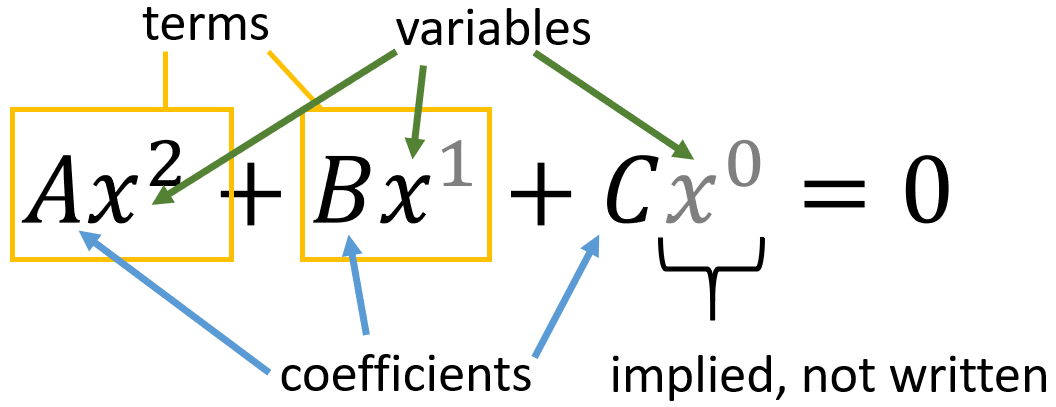
\includegraphics[width=0.6\textwidth]{poly}
\end{center}
The prefix \textit{poly} means many, and polynomials are not limited to three terms. The general form of a polynomial can be written as:
$$ A_1x^n+A_2x^{n-1}+A_3x^{n-2}+\dots+A_nx^1+C=0 $$
where the terms are written in decreasing powers of $x$, with
\vspace{-0.5cm}\begin{itemize}
	\setlength\itemsep{0em}
	\item $n\ge 0, n\in \mathbb{Z}$. This means the exponents must be integers.
	\item $A_1, \dots, A_n$ are real numbers.
	\item $C$ is a constant.
	\item The order or degree of the polynomial is $n$ (the highest exponent).
	\item Here, $x$ is the variable. You may have more than one variable in a polynomial, for example $4x^2+y-xy+4$ is a valid polynomial.
\end{itemize}
 
 
 %%%%%%%%%%%%%%%%%%%%%%%%%%%%%%%%%%%%%%%%%%%%
 \section{Systems of Equations}\label{sec:systemsOfEquations}
 A system of equations means having more than one relationship represented within a common context. Revenue and costs may have different functions but both relate to the same product. We will study systems composed of two equations and two unknowns. Systems with more equations and more variables are possible and will be covered in future courses. Three approaches to solve systems of equations will be covered here:
 \begin{multicols}{3}
  \begin{itemize}
 	\setlength\itemsep{0em}
 	\item graphing\columnbreak
 	\item elimination\columnbreak
 	\item substitution
 \end{itemize}
\end{multicols}
It helps if you can visualise the shape of the two functions so that the meaning of the solution is clear in your mind. Later in the course we will find the area between two curves using integration where the intersection of these two curves represents the solution to a system of two equations. See section XX.
 
 We know that linear equations in two variables are represented by straight lines. Straight
 lines will always intersect unless they are parallel. The coordinates of the point of intersection of the straight lines is called the solution. you could use a graphical method or one of the two algebraic methods (substitution or elimination) to find the solution.  We will start with a graphical method. 
 
 \example Find the solution to the set of linear relationships given by:
 $$2y=x-4$$
 $$y=\frac{x}{4}$$
  \begin{multicols}{2}
 \solution Here we have two linear equations (we know they are linear because the highest exponent is 1) and if the lines intersect, that point of intersection represents a solution. 
 	
 	From the plot we can see the point of intersection is $(8,2)$. Therefore the solution to the system of linear equations is $(8,2)$. Try plotting the lines yourself with \desmos.
 	
 	
 	Its not always convenient to graph a system of equations to find the solution; you may not have access to a computer, or the solution may not be integers. Solving by direct substitution is the next method.
 	\columnbreak
 \begin{center}
 \begin{tikzpicture}
 \begin{axis}[
 grid=both,
 minor tick num=1,
 axis lines=center,
 xmax=10,xmin=-2,
 ymax=3,ymin=-3,
 xlabel=$x$,ylabel=$y$,
 ticklabel style={fill=white},
 ]	
 \node[anchor=south,fill=white] at (axis cs:2,1) {$y=\frac{x}{2}-4$};
 \node[anchor=south,fill=white] at (axis cs:7.25,0.5) {$y=\frac{x}{4}$};
 \addplot [<->,domain=-2:10,thick, samples=100, black] {0.5*x-2};
 \addplot [<->,domain=-2:10,thick, samples=100, black] {0.25*x};
 \addplot[mark=*] coordinates {(8,2)};
 \end{axis}	
 \end{tikzpicture}			
\end{center}
\end{multicols}
 \subsection*{Solution by Substitution}
 \example Consider the system of equations
 \begin{align}x^{2} +y^{2} &  = 25 \tag{1} \\
 3 y +x &  = 15 \tag{2}\end{align}
 \solution Without knowing what the functions look like or plotting them, we can isolate a variable and substitute it into the other equation. Rearrange equation (2) to isolate $x$ and substitute into equation (1):
$$x =  15 -3 y $$
 Equation (1) becomes
 \begin{align*}(15-3y)^2+y^2 &  =  25 \tag{expand and simplify}\\
 225-90y+9y^2+y^2&=25\\
 10 y^{2} -90 y +200 &  =  0 \tag{divide by 10}\\
 y^{2} -9 y +20 &  = 0 \tag{factor the quadratic}\\
 \left (y -5\right ) \left (y -4\right ) &  =  0 \\
 \text{Either }\quad y -5 &  =  0\quad\text{ so }\quad y =5 \\
 \text{or }\quad y -4 &  =  0\quad\text{ so }\quad y =4\end{align*}
 
Lastly, back-substitute the $y-$values into equation (2): 
 
 When $y =5$, $3 y +x =15 \leadsto 15 +x =15 \Longleftrightarrow x =0$. This means $\left (0 ,5\right )$ is a solution. 
 
 When $y =4$, $3 y +x =15 \leadsto 12 +x =15 \Longleftrightarrow x =3$. This means $\left (3 ,4\right )$ is a solution. 
 Note there are two solutions here. Verify by graphing the functions.
\subsection*{Solution by Elimination} 
The third method is called elimination and works by eliminating one of the variables from the equation set, then solving for the other variable.

\example Solve the system by the method of elimination:
\begin{align*}
4x-3y&=5\tag{1}\\
4x+\phantom{1}y&=1\tag{2}
\end{align*}
\solution If we subtract equation (2) from equation (1) columnwise then the $x$ term is eliminated because $4x-4x=0$.
\[\begin{array}{lrl}
  			 &4x-3y	         &=5 \\[\jot]
 -\phantom{1}&4x+\phantom{1}y&=1 \\
\cmidrule{2-3}
 & 0x-4y &=4  \\[\jot]
\end{array}\]
Now there is one equation with one unknown: $-4y=4$ so $y=-1$. Back-substitute into either previous equation to solve for $x=\frac{1}{2}$. Therefore the solution is $x=\frac{1}{2},y=-1$.\\
\rule{6.8cm}{0.5pt}\\
\example Solve the system by the method of elimination:
\begin{align*}
3a-7b&=-3\tag{1}\\
b&=\frac{6a-4}{2}\tag{2}
\end{align*}
\solution The first step is to write the equations so the variables line up in columns. Multiply equation (2) by 2 to get $2b=6a-4$ and rearrange the terms to match equation (1). 

\begin{minipage}[t]{0.3\linewidth}
The system now looks like:
\begin{align*}
3a-7b&=-3\tag{1}\\
6a-2b&=\phantom{1}4\tag{3}
\end{align*}
We can't eliminate any variables because the coefficients are different. 
\end{minipage}
\hspace{\fill}
\begin{minipage}[t]{0.3\linewidth}
Multiply equation (1) by 2.
\begin{align*}
6a-14b&=-6\tag{4}\\
6a-\phantom{1}2b&=\phantom{1}4\tag{3}
\end{align*}
\end{minipage}
\hspace{\fill}
\begin{minipage}[t]{0.3\linewidth}
Now calculate (4) $-$ (3).	
\[\begin{array}{lrl}
			&	       6a-14b&=-6			\\[\jot]
-\phantom{1}&6a-\phantom{1}2b&=\phantom{1}4 \\
\cmidrule{2-3}
& 0+12b&=10  \\[\jot]
\cmidrule{2-3}
& b&=\frac{5}{6}  \\[\jot]
\end{array}\]	
\end{minipage}

Back-substitute $b$ into equation (1) to solve for $a$: $3a-7(\frac{5}{6})=-3$. Verify that $a=\frac{17}{18}$.	
	
 \section*{Special Cases}
  \begin{multicols}{2}
  Consider the parallel lines shown. What is the solution to this system? Parallel lines will never meet by definition and so will have no point of intersection. In this case the system has no solution -- which is a perfectly valid solution! Notice the slope of both the lines is $\frac{1}{3}$ which means they are parallel.
  
  Sometimes the two equations will be two different representations of the same line. Imagine two line plotted on top of one another. In this case the system has an infinite number of solutions because every single point on the first function is also on the second function. 
 	\columnbreak
 	\begin{center}
 		\begin{tikzpicture}
 		\begin{axis}[
 		grid=both,
 		minor tick num=1,
 		axis lines=center,
 		xmax=5,xmin=-5,
 		ymax=3,ymin=-4,
 		xlabel=$x$,ylabel=$y$,
 		ticklabel style={fill=white},
 		]	
 		\node[anchor=south,fill=white] at (axis cs:2,-3) {$y=\frac{x}{3}-2$};
 		\node[anchor=south,fill=white] at (axis cs:2.6,0) {$y=\frac{x}{3}+0.5$};
 		\addplot [<->,domain=-5:5,thick, samples=100, black] {0.333*x-2};
 		\addplot [<->,domain=-5:5,thick, samples=100, black] {0.333*x+0.5};
 		\end{axis}	
 		\end{tikzpicture}			
 	\end{center}
 \end{multicols}
 
 \example If you start with a linear equation such as $y -2 x =3$ and multiply each term by a constant you will get an equivalent equation. If you multiply the equation by another number you
 will get a further equivalent equation.
 \[y -2 x =\phantom{-}3 \]
 Multiply by $2$
\[2 y -4 x =\phantom{-}6\]
 Multiply by $-3$
\[-3y +6x = -9\]
\solution We know these are both just different ways of writing the original equation $y -2 x =3$ or $y =2 x +3$. To say the system has an infinite number of solutions we are really saying every point on $y =2 x +3$ is a solution. 
 
 \section*{Guidelines for Solving Systems of Equations}
 These guideline provide a useful way to tackle any problems where equations are involved. 
 \begin{tcolorbox}
 	
  \begin{enumerate}\setlength\itemsep{0em}
 	\item Identify the variables. We often call them $x$ and $y$, but you may chose any name or letter you want. 	
 	\item Express all unknown quantities in terms of the variables. 	
 	\item Set up a system of equations using the facts provided by the problem.	
 	\item Solve the system of equations and use the solution to check it satisfies the conditions of the
 	problem. Write a sentence describing the answer to the original problem.  
 \end{enumerate}
\end{tcolorbox}
 
 \example It takes a boat travelling downstream 1 hour to cover the 20 mile distance. On the return trip it take the boat 2.5 hours. What is the speed of the boat and the speed of the current?\medskip\\
 \solution This is about a boat travelling with the current and against the current and depends on you knowing that velocities are vectors that can be added and subtracted. Let the speed of the boat be $x$ \mbox{mi}$/$\mbox{h} and the speed of the current be $y$ \mbox{mi}$/$\mbox{h}. 
 	\begin{align*}\text{Upstream speed} &  =  x -y \\
 	\text{Downstream speed} &  =  x +y\end{align*}
 	\begin{align}\text{Speed} &  =  \frac{\text{Total distance}}{\text{Total time}} \nonumber  \\
 	\text{so Total distance} &  =  \text{Speed} \times \text{Total time} \nonumber  \\
 	20 \textrm{ miles } &  =  \left (x +y\right ) \times 1 \textrm{ hour} \nonumber  \\
 	20 &=x +y \tag{1} \\
 	\text{Also}\quad 20 \textrm{ miles }&  =  \left (x -y\right ) \times \frac{5}{2} \textrm{ hours}\nonumber  \\
 	8 &=x -y \tag{2}\end{align}
 Now we can add equations (1) and (2) and $y$ is eliminated
 \begin{align*}28 &  =  2 x \\
 x &  =  14\end{align*} \\
 Back-substitute into either equation (1) or (2) to solve for $y =  6$.\medskip\\
 \textbf{Check:} The boat travels at 14 $\mbox{mi}$/$\mbox{h}$ and the current travels at 6 $\mbox{mi}$/$\mbox{h}$ so the effective speed of the boat is 20 $\mbox{mi}$/$\mbox{h}$. At 20 $\mbox{mi}$/$\mbox{h}$ the 20 $\mbox{mi}$ trip took $1$ $\mbox{h}$. Upstream the speed is 8 $\mbox{mi}$/$\mbox{h}$.
 \begin{align*}\text{Total time} &  =  \frac{\text{Total distance}}{\text{Speed}} \\
 &  =  \frac{20}{8} =\frac{5}{2} \text{ h}\end{align*}
 
 Therefore the speed of the boat is 14 $\mbox{mi}$/$\mbox{h}$ and the speed of the current is 6 $\mbox{mi}$/$\mbox{h}$. 

%------------------------------------------------------------------- 
% Algebra Exercises in a separate file
%-------------------------------------------------------------------
\section{Chapter Exercises}
\subimport{}{AlgebraExercises}

\chapter{Trigonometry}
In the first half of this chapter the three trigonometric functions (sine, cosine and tangent) will be viewed as functions of angles. The second half of the chapter will approach trigonometry as functions of real numbers.
%---------------------------------------------------
% pythagorean theorem
%---------------------------------------------------
\section*{Pythagoras}
Pythagoras is one of the most well known historical figures in mathematics and philosophy, primarily for his eponymous theorem. Given a right-angled triangle, the square of the hypotenuse equals the sum of the squares of the other sides.
\begin{tcolorbox}[colback=white]
	\begin{multicols}{2}
		\begin{center}
			The Pythagorean Theorem:\\
			
			\vspace{1cm}$a^2+b^2=c^2$
		\end{center}
\columnbreak
\begin{center}
	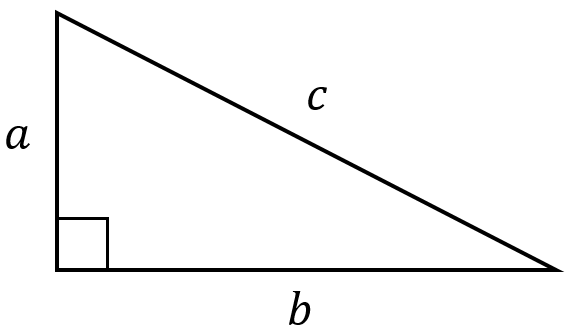
\includegraphics[width=6cm]{trigPythagoras}
\end{center}
	\end{multicols}
\end{tcolorbox}
This diagram will be the basis for a lot of our study of triangles. We will return to the Pythagorean theorem in section~\ref{sec:identities} when discussing some special trigonometry relationships.
%---------------------------------------------------
% the unit circle and radians
%---------------------------------------------------
\section{The Unit Circle}
It should come as no surprise that the convention for measuring angles should be the same as for measuring
the distance around the perimeter of the unit circle.. An angle is measured in degrees and is the amount of
rotation between two rays about a vertex. If the vertex is placed at the point $\left (0 ,0\right )$ and one ray is placed along the positive $x$-axis then we let the second ray go through the point $P (x ,y)$ on the unit circle so that the relationship between the angle and the arc length $t$ can be established. The convention is that the positive direction for measuring
angles is anticlockwise and the negative direction for measuring angles is clockwise. You will be aware that one complete cycle measures \ang{360}. One degree therefore is $\frac{1}{360}$\ of one complete cycle. In this subject the word revolution is often used instead of cycle. Other terms with which you might be familiar are ``a quarter turn" for \ang{90} and ``a half turn" for \ang{180}. 

If you draw a unit circle (centre $\left (0 ,0\right )$ radius $1$) then you can draw the ray through any terminal point and show the relationship between $t$ and the angle at the vertex $\left (0 ,0\right )$. 

Definition: If the unit circle is drawn and the distance $t$ is measured around the perimeter from $\left (1 ,0\right )$ to the point $P (x ,y)$ then we say the angle is measured as $t$ \emph{radians}. 

The abbreviation for radians is \textit{rad}. This abbreviation will be used in the examples.
Some books uses the term ``angles in standard position" to describe this situation. We
will not define this term unless it is unavoidable and will stick to rad.

\columnsep =30pt
\begin {multicols}{2}
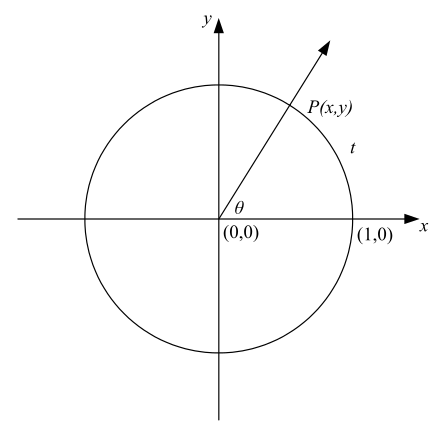
\includegraphics[width=6cm]{L4SZ281A}
\columnbreak

Using the language of geometry, the unit circle is cut by two rays one through the points $\left (0 ,0\right )$ and $\left (1 ,0\right )$ and the other through the points $\left (0 ,0\right )$ and $P \left (x ,y\right )$. 

$t$ is referred to as "the length of the arc". The angle $\theta $ between the two rays is referred to as "the angle \emph{subtended} at the point $\left (0 ,0\right )$". We will often leave out the word "subtended" however as it is implied. 
\end {multicols}
We can say therefore that the angle measured in radians is related to the same angle measured in degrees. the relationship between these two measures must be understood and must be able to be derived. 

\subsection*{Relationship between Degrees and Radians}
One complete revolution is \ang{360} if the angle is measured in degrees and $2 \pi $ if the angle is measured in radians. So
\begin{align*}2 \pi \text{}\mbox{rad} &  =  \ang{360} \\
\text{or\  \ }\pi \text{}\mbox{rad} &  =  \ang{180}
\end{align*}
You should derive this formula whenever you are asked to convert degrees to radians or radians
to degrees. 

\example
(a) Convert \ang{36} to radians 
(b) Convert $\frac{\pi }{3}$ $\mbox{rad}$ to degrees 
(c) Convert $1$ $\mbox{rad}$ to degrees \medskip\\

\solution \begin{tasks}[before-skip = {0ex} , after-skip={-5ex}](3)
\task \begin{align*}\ang{180}  &  =  \pi \text{}\mbox{rad} \\
\ang{1}  &  =  \frac{\pi }{180}\text{}\mbox{rad} \\
\ang{36}  &  =  \frac{\pi }{180} \times 36 =\frac{\pi }{5}\text{}\mbox{rad}\end{align*}
\task
\begin{align*}\pi  \mbox{rad} &  =  \ang{180}  \\
\frac{\pi }{3} \mbox{rad} &  = \frac{\ang{180} }{3} =\ang{60} \end{align*}
\task
\begin{align*}\pi  \mbox{rad} &  =  \ang{180} \\
1 \mbox{rad} &  =  \frac{\ang{180} }{\pi } \\
 &  \approx   \ang{57.29577951}  \\
 &  \approx   \ang{57.3} \end{align*}
\end{tasks}
Note the similarity between the answers to (b) and (c). This is because $\frac{\pi }{3} =1.047197551$ so you would expect the values in degrees to be similar.  With this terminology we leave out the word measured when we talk about measuring angles. We say ``the angle is $\ang{60} $" when we mean it has been measured as $\ang{60} $ or ``the angle is $\frac{\pi }{3}$" to mean it has been measured as $\frac{\pi }{3}$ $\mbox{rad}$. Notice we always put in the degree symbol and often omit the units when the angle is measured in radians. Should units be omitted assume the angle is measured in radians. We often use the Greek symbol $\theta $\ for the angle subtended at the centre of the unit circle so $\theta  =\ang{60} $ or $\theta  =\frac{\pi }{3}$ are further examples of terminology that is commonly used.

\subsection*{Arc Length}
Let $\theta $ be the angle subtended at the centre for the ends of an arc of any circle then the fraction of the circumference of the circle is $\frac{\theta }{2 \pi }$ if $\theta $ is measured in radians and $\frac{\theta }{\ang{360}}$ if $\theta $ is measured in degrees. 

The length of the circumference of any circle whose radius is $r$ is $2 \pi  r$. If $\theta $ is measured in radians
\begin{equation*}\text{Length of arc} =\frac{\theta }{2 \pi } \times 2 \pi  r =\theta  r\text{or}r \theta 
\end{equation*}

If $\theta $ is measured in degrees
\begin{equation*}\text{Length of arc} =\frac{\theta }{\ang{360}} \times 2 \pi  r
\end{equation*}

The simplicity of the first formula shows why working with radians is preferred. 

\example Find the length of an arc that subtends an angle of \ang{45} at the centre of a circle whose radius is 9 cm. 

\solution \begin{tasks}[counter-format=(tsk[1]),before-skip = {0ex},after-skip={-5ex}](2)
	\task Method 1:\begin{eqnarray*}\text{Length of arc} &  = & \frac{\theta }{360 \mbox{{\ensuremath{{}^\circ}}}} \times 2 \pi  r \\
	&  = & \frac{45}{360} \times 2 \pi  \times 9 \\
	&  = & 2.25 \pi \text{}\mbox{cm} \\
	&  \approx  & 7.07\text{}\mbox{cm}\end{eqnarray*}
If an exact answer is required you should\\ leave the answer as $2.25 \pi $ $\mbox{cm}$. (Or $\frac{9 \pi }{4}$ $\mbox{cm}\text{.}$) 

\task Method 2: Change degrees to radians first
\begin{eqnarray*}180 \mbox{{\ensuremath{{}^\circ}}} &  = & \pi \text{}\mbox{rad} \\
	1 \mbox{{\ensuremath{{}^\circ}}} &  = & \frac{\pi }{180} \\
	45 \mbox{{\ensuremath{{}^\circ}}} &  = & \frac{\pi }{180} \times 45 \\
	&  = & \frac{\pi }{4}\end{eqnarray*}
Now, the length of arc $= r \theta = 9 \times \frac{\pi }{4} =\frac{9 \pi }{4}\text{}\mbox{cm}$.
\end{tasks}
%---------------------------------------------------
% Right-Angled Triangles: trig ratios
%---------------------------------------------------
\section{Right-Angled Triangles}
A right angled triangle is uniquely defined, if as well as the \ang{90} angle, you are given one side and one angle or two sides. To be given two angles does is not enough information as the scale of the triangle is not known. The sides of the triangle have names with respect to the angle of interest, $\theta$ in the diagram. 
\begin{multicols}{2}
\begin{center}
	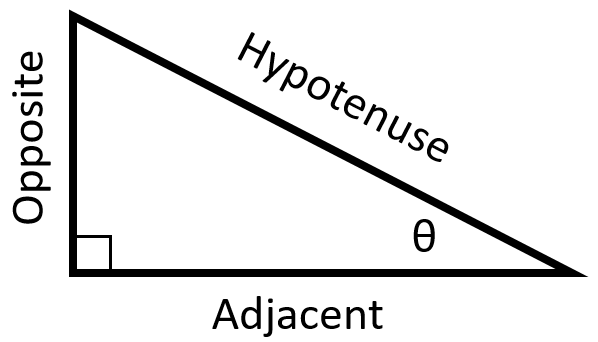
\includegraphics[width=5.5cm]{rightTriangle}
\end{center}
\columnbreak
Notice that if $\theta$ changes, then the sides opposite and adjacent are reversed. These side names are helpful in defining the trigonometric ratios of sine, cosine and tangent. \end{multicols}

The phrase \textbf{SOH-CAH-TOA} is useful to remember the ratios.
\begin{tcolorbox}
\begin{equation*}\text{sine }  \theta  =\frac{\text{opposite}}{\text{hypotenuse}}\text{;}\qquad\text{cosine }  \theta  =\frac{\text{adjacent}}{\text{hypotenuse}}\text{;}\qquad\text{tangent }  \theta  =\frac{\text{opposite}}{\text{adjacent}}
\end{equation*}\medskip
\hspace{2.5cm}S O H\hspace{3cm}C A H\hspace{4cm}T O A
\end{tcolorbox}

%----------------------------------------------------
\begin{multicols}{2}
	\example Find the unknown side $x$\\
	\begin{center}
		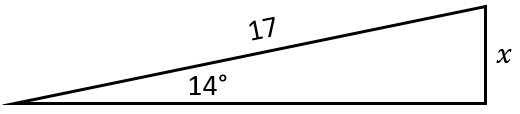
\includegraphics[width=8cm]{trigSide1}
	\end{center}

	\columnbreak
\solution Write the sine ratio and solve for $x$.\\
\begin{align*}\sin 14 &= \frac{x}{17}\\
x&=17\sin 14\\
x&=4.11\end{align*}
\end{multicols}

\begin{multicols}{2}
\example Find the unknown side $x$\\
\begin{center}
	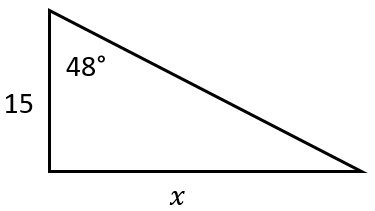
\includegraphics[width=6cm]{trigSide2}
\end{center}
	\columnbreak
\solution Write the tangent ratio and solve for $x$.
\begin{align*}\tan 48 = \frac{x}{15}\\
x=15\tan 28\\
x=16.7\end{align*}
\end{multicols}

The calculator gives approximate values of the trigonometric ratios. You must look at your question to check whether angles are in degrees or radians and ensure the calculator is first set in the right mode. Questions where degrees are to be used will give angles marked with a $^\circ$ symbol. 


When solving for an angle on your calculator you select the appropriate trigonometry ratio and use the \emph{shift} button with sin, cos or tan to find $\sin ^{ -1}$, $\cos ^{ -1}$ or $\tan ^{ -1}$. 
%----------------------------------------------------
\begin{multicols}{2}
	\example Find the unknown angle $x$\\
	\begin{center}
		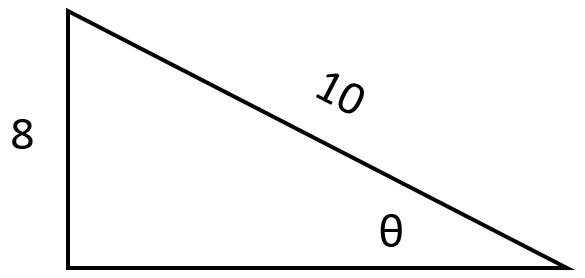
\includegraphics[width=7cm]{trigAngle1}
	\end{center}
	
	\columnbreak
	\solution Write the sine ratio and solve for $\theta$.\\
	\begin{align*}\sin \theta &= \frac{8}{10}\\
	\sin\theta&=0.8\\
	\theta&=\sin^{-1}(0.8)\\
	\theta&=\ang{53.1}
	\end{align*}
\end{multicols}
\clearpage
\begin{multicols}{2}
	\example Find the unknown angle $x$\\
	\begin{center}
		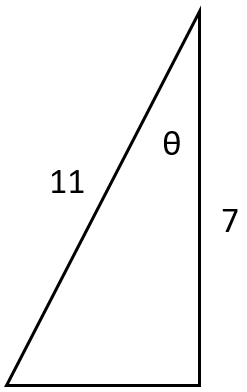
\includegraphics[width=3cm]{trigAngle2}
	\end{center}
	\columnbreak
	\solution Write the cosine ratio and solve for $\theta$.
	\begin{align*}\cos \theta = \frac{7}{11}\\
	\theta=\cos^{-1} \left(\frac{7}{11}\right)\\
	\theta=\ang{50.5}
	\end{align*}
\end{multicols}
%----------------------------------------------------
\example The height of a steep cliff is to be measured from a point on the opposite side of the river. The following diagram shows the measurements taken. Estimate the height of the cliff.
\begin {multicols}{2}
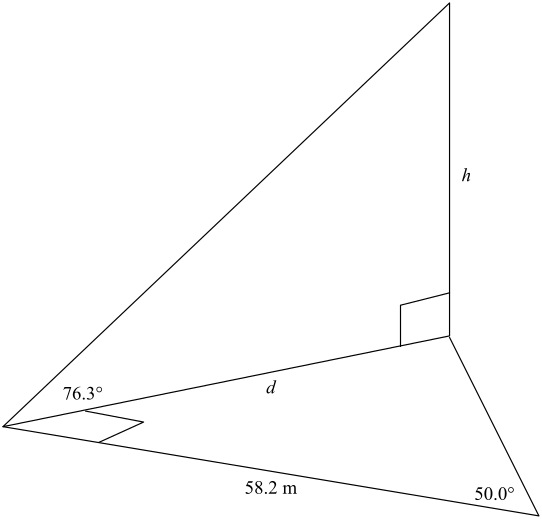
\includegraphics[width=8cm]{L4SZ281H}
\columnbreak\\
\solution 
\begin{align*}\frac{d}{58.2} &  =  \tan  \ang{50.0}  \\
d &  =  58.2 \times \tan  \ang{50.0}  \\
\frac{h}{d} &  =  \tan  \ang{76.3}  \\
h &  =  d \times \tan  \ang{76.3}  \\
 &  =  58.2 \times \tan  \ang{50.0}  \times \tan  \ang{76.3}  \\
 &  \approx   284.526397 \\
 &  \approx   284.5 \mbox{m}\end{align*}
\end {multicols}\rule{6.8cm}{0.5pt}\\

%----------------------------------------------------
\example To estimate the height of a mountain above a level plane the angle of elevation of the top of the mountain is measured to be $\ang{30} $. $600 \mbox{m}$ closer to the mountain across the plane it is found that the angle of elevation is $\ang{36} $. Estimate the height of the mountain. \\
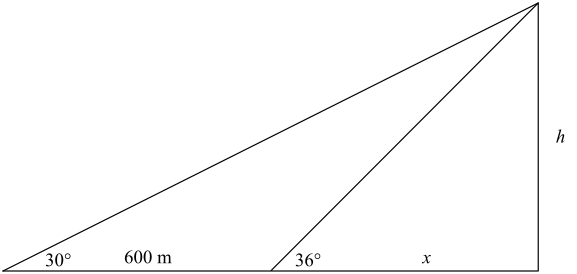
\includegraphics[width=10cm]{L4SZ281I}\\
\solution
\begin{equation*}\frac{h}{x} =\tan  \ang{36} \text{and}\frac{h}{x +600} =\tan  \ang{30} 
\end{equation*}
We want $h$ so we eliminate $x$ between these two equations
\begin{align*}x &  =  \frac{h}{\tan  \ang{36} }\text{and}x +600 =\frac{h}{\tan  \ang{30} } \\
\frac{h}{\tan  \ang{30} } &  =  \frac{h}{\tan  \ang{36} } +600 \\
\frac{h}{\tan  \ang{30} } -\frac{h}{\tan  \ang{36} } &  =  600 \\
h \left (\frac{1}{\tan  \ang{30} } -\frac{1}{\tan  \ang{36} }\right ) &  =  600 \\
h \genfrac{(}{)}{}{}{\tan  \ang{36}  -\tan  \ang{30} }{\tan  \ang{30}  \tan  \ang{36} } &  =  600 \\
h &  =  600 \times \frac{\tan  \ang{30}  \tan  \ang{36} }{\tan  \ang{36}  -\tan  \ang{30} } \\
 &  \approx   600 \times 2.811603815 \\
 &  \approx   1687 \mbox{m}\end{align*}

%---------------------------------------------------
% identities
%---------------------------------------------------
\subsection*{Identities}\label{sec:identities}
The unit circle has equation $x^{2} +y^{2} =1$ and we define $x =\cos  \theta$ and $y =\sin  \theta$ so
\begin{equation*}x^{2} +y^{2} =1 \leadsto \left (\cos  \theta\right )^{2} +\left (\sin  \theta\right )^{2} =1
\end{equation*}
This is always written
\begin{tcolorbox}\[\sin ^{2} \theta +\cos ^{2} \theta =1\]
\end{tcolorbox}
This is an \emph{identity} which means it is true for all values of $\theta$. There are many identities in trigonometry, we will only use the Pythagorean identity (above) and one more.
Given $\sin =\frac{\text{opp}}{\text{adj}}$ we can solve for $\text{opp}=(\sin)(\text{hyp})$. Similarly from cosine:  $\text{adj}=(\cos)(\text{hyp})$. Substituting these into the tangent relationship:
\begin{tcolorbox}\[\tan=\frac{\text{opp}}{\text{adj}}=\frac{(\sin)(\text{hyp})}{(\cos)(\text{hyp})}=\frac{\sin}{\cos}\]
\end{tcolorbox}
The sine and cosine law are two more unique relationships that we will cover in section~\ref{sec:applications}.

%---------------------------------------------------
% trig functions
%---------------------------------------------------
\subsection*{All Students Take Calculus}
In the previous section the angles were between $\ang{0} $ and $\ang{90} $. In this section the angles can take any value. Initially we consider angles between $\ang{0} $ and $\ang{360} $ and relate these to the radian measure between $0$ and $2 \pi $. We remind you that angles are measured anticlockwise from the positive $x$-axis. 

If the point $P (x ,y)$ is in the first quadrant, $\theta $ is the angle between $OP$ and the positive $x$-axis and we complete the right triangle then we have created the following situation.  

\begin {multicols}{2}
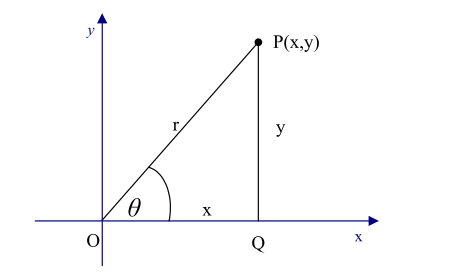
\includegraphics[ width=3.774in, height=2.3454in,]{L4SZ281S}

Let the hypotenuse be $r$ then
\begin{equation*}r =\sqrt{x^{2} +y^{2}}
\end{equation*}
Therefore
\begin{equation*}\sin  \theta  =\frac{y}{r}\text{}\cos  \theta  =\frac{x}{r}\text{and}\tan  \theta  =\frac{y}{x}
\end{equation*}
\end {multicols}
\begin {multicols}{2}
We now let $\theta $ be any angle and define sine, cosine and tangent in the same way. For instance
if $P (x ,y)$ is in the second quadrant:    

$\sin  \theta  =\frac{y}{r}$ because $y$ is positive $\sin  \theta $ will be positive. ($r$ is positive by convention.) 

$\cos  \theta  =\frac{x}{r}$ because $x$ is negative $\cos  \theta $ will be negative. 

$\tan  \theta  =\frac{y}{x}$ because $y$ is positive and $x$ is negative $\tan  \theta $ will be negative. 
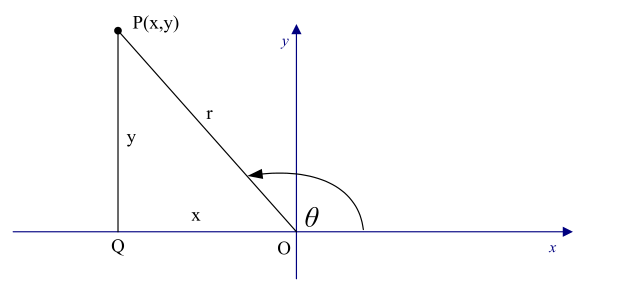
\includegraphics[ width=3.9868in, height=1.8161in,]{L4SZ281T}
\end{multicols}
This pattern can be extended to quadrants 3 and 4. The mnemonic (\textbf{A}ll \textbf{S}tudents \textbf{T}ake \textbf{C}alculus) might help you remember which one is positive although you can always work it out if you need to. 

The value of a trigonometric function consists of two parts the numerical part and the sign. you must get both parts correct. In the previous section you related the values of a terminal point to another point in the first quadrant. A point on the unit circle could be in any one of the four quadrants. 

\qquad \qquad \qquad \qquad
\begin{tabular}[c]{|c|c|c|c|c|c|}\hline
	Quadrant  & $x$-coordinate  & $y$-coordinate  & $\cos $  & $\sin $  & $\tan $  \\
	\hline
	$1$  & $ +$  & $ +$  & $ +$  & $ +$  & $ +$  \\
	\hline
	$2$  & $ -$  & $ +$  & $ -$  & $ +$  & $ -$  \\
	\hline
	$3$  & $ -$  & $ -$  & $ -$  & $ -$  & $ +$  \\
	\hline
	$4$  & $ +$  & $ -$  & $ +$  & $ -$  & $ -$  \\
	\hline
\end{tabular}

Some people learn this as a mnemonic All sin tan cos. (Meaning all are positive in the first quadrant, only sine is positive in the second quadrant, only tangent is positive in the third quadrant and only cosine is positive in the fourth quadrant.) 

\subsection*{The Area of a Triangle}
The fundamental formula for the area of a triangle is $\text{Area} =\frac{1}{2} \times \text{base} \times \text{height}$ Using the trigonometric functions the height can be replaced and the formula becomes:
\begin{equation*}\text{Area} =\frac{1}{2} \times \text{product of two sides} \times \text{sine of the included angle}
\end{equation*}
The formula is particularly easy to remember in symbolic form. Let the triangle have vertices $A$, $B$ and $C$, so the the sides opposite these angles are $a$, $b$ and $c$ respectively. Then the area can be expressed symbolically as
\begin{equation*}\text{Area} =\frac{1}{2} a b \sin  C =\frac{1}{2} b c \sin  A =\frac{1}{2} a c \sin  B
\end{equation*}

\columnsep =30pt
\begin {multicols}{2} 
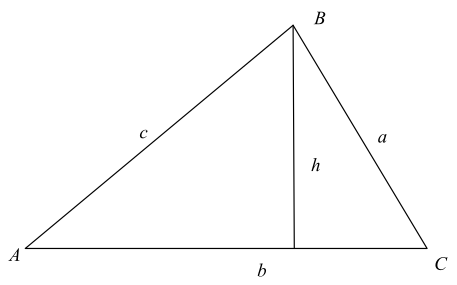
\includegraphics[width=8cm]{L4SZ281U}

\begin{align*}\sin  A &  = \frac{h}{c}\text{ and }h =c \sin  A \\
\text{Area} &  =  \frac{1}{2} \times \text{base} \times \text{height} \\
 &  =  \frac{1}{2} \times b \times c \sin  A =\frac{1}{2} b c \sin  A
 \end{align*}
\end {multicols}
It depends where you draw $h$ and which angle you choose to use as to which formula you finish up with. The key point to remember is $b$ and $c$ are two sides and $A$ is the angle between them. The triangle above shows $A$ as an acute angle (between $\ang{0}$ and $\ang{90} $). If the angle is obtuse (between $\ang{90} $ and $\ang{180} $) the formula still holds. 
\begin{multicols}{2}
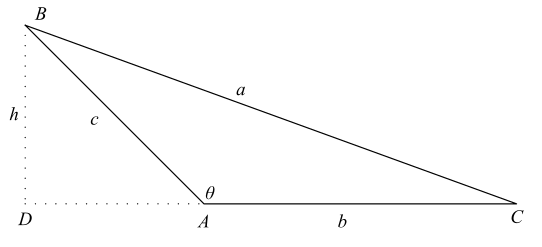
\includegraphics[ width=8cm]{L4SZ281V}
The angle is in the second quadrant and $\sin  (180 -\theta ) =\sin  \theta $, so $\sin  (180 -\theta ) =\frac{h}{c}$ can be written as $\sin  \theta  =\frac{h}{c}$ or $h =c \sin  \theta $ or $h =c \sin  A$ where $A$ is obtuse. So the area is $\frac{1}{2} b c \sin  A$ 
\end{multicols}
\example A triangle has two sides of $5 \mbox{cm}$ and $8 \mbox{cm}$ and the angle between them is $\ang{150} $. Find its area.\medskip\\
\solution
\begin{equation*}\text{Area} =\frac{1}{2} \times 5 \times 8 \times \sin  \ang{150} 
\end{equation*}

It helps to remember that $\sin  150 =\sin  30 =\frac{1}{2}$
\begin{equation*}\text{Area} =\frac{1}{2} \times 5 \times 8 \times \frac{1}{2} =10 \text{ cm}^{2}
\end{equation*}

%---------------------------------------------------
% TRIG FUNCTIONS & GRAPHS
%---------------------------------------------------
\section{Trig Functions of Real Numbers}
In this next part of the chapter the three main trigonometric functions (sine, cosine and tangent) will be studied. They will be viewed as functions of real numbers rather than angles. The trigonometric functions defined in these two ways are identical and there is a simple rule connecting the domains. Why do we show you the two approaches? Trigonometry will be used to solve a variety of problems and these can be divided into two groups, dynamic problems and static problems. When dynamic problems (such as problems involving motion) are being solved real numbers will be used. When static problems (such as finding distances and angles for triangles) are being solved angles will be used. 

%---------------------------------------------------
% trig graphs
%---------------------------------------------------
%\section{Trigonometric Functions}
You should be familiar with the fundamental graphs of $y =\sin  x$ and $y =\cos  x$. These graphs are the basis of this section. \Desmos can easily show you the shape of $y =\sin  x$ and $y =\cos  x$ so if you are asked to draw a rough sketch of these curves you should plot a few key points and draw a smooth curve between them. You will usually be given the required domain however if you are not you would choose to draw these for one complete cycle ($0 -2 \pi $). To sketch $y =\sin  x$ it is enough to select as key points $x =0$, $\frac{\pi }{2}$, $\pi $, $\frac{3 \pi }{2}$, $2 \pi $. 


\begin{tabular}[c]{|l|l|l|l|l|l|}\hline
	$x$  & $0$  & $\frac{\pi }{2}$  & $\pi $  & $\frac{3 \pi }{2}$  & $2 \pi $  \\
	\hline
	$y =\sin  x$  & $0$  & $1$  & $0$  & $ -1$  & $0$  \\
	\hline
\end{tabular}

Similarly to sketch $y =\cos x$ the same values of $x$ give: 


\begin{tabular}[c]{|l|l|l|l|l|l|}\hline
	$x$  & $0$  & $\frac{\pi }{2}$  & $\pi $  & $\frac{3 \pi }{2}$  & $2 \pi $  \\
	\hline
	$y =\cos  x$  & $1$  & $0$  & $ -1$  & $0$  & $1$  \\
	\hline
\end{tabular}

You will be aware that these curves repeat this pattern every $2 \pi $ where $x$ extends in both the positive and negative directions. $0$ to $2\pi $ represents one complete cycle. Mathematically we say
\begin{align*}\sin  \left (x +2 n \pi \right ) &  = \sin  x\text{\  for any integer }n \\
	\cos  \left (x +2 n \pi \right ) &  = \cos  x\text{\  for any integer }n\end{align*}

Aside: instead of ``for any integer $n$" we can write $ \forall n \in \mathbb{Z}$. A function that displays this characteristic is described as \emph{periodic} and for $y =\sin x$ and $y =\cos x$ the \emph{period} is $2 \pi $. 

\subsection{Transformations}
The following six transformations can be applied to any function including sine, cosine, and tangent. 
\begin{tasks}[style=itemize](3)
\task Vertical shift 
\task Horizontal shift 
\task Vertical stretch 
\task Horizontal stretch 
\task Reflection in the $x$-axis 
\task Reflection in the $y$-axis 
\end{tasks}

\example Sketch $y =\sin  \left (x -\frac{\pi }{2}\right ) +3$. This may be considered as a sine curve shifted $\frac{\pi }{2}$ units to the right. Note for periodic functions like a sine wave a horizontal shift is called a \textit{phase shift}. and $3$ units upwards.\\ 
\solution 1. Beginning with the special points for $\sin x$, a table shows the evolution of the points. \\
\begin{tabular}{llllllc}\cmidrule{1-6}
	$x$  & $0$  & $\frac{\pi }{2}$  & $\pi $  & $\frac{3 \pi }{2}$  & $2 \pi $ & $\leftarrow x$-values, plot these \\
	\cmidrule{1-6}
	$\sin  x$  & $0$  & $1$  & $0$  & $ -1$  & $0$ & \\
	\cmidrule{1-6}
	$\sin  \left (x -\frac{\pi }{2}\right )$  & $ -1$  & $0$  & $1$  & $0$  & $ -1$&  \\
	\cmidrule{1-6}
	$\sin  \left (x -\frac{\pi }{2}\right ) +3\qquad$  & $2$  & $3$  & $4$  & $3$  & $2$&$\leftarrow y$-values, plot these  \\
	\cmidrule{1-6}
\end{tabular}

2. Plot the transformed values with the original special points and connect with a smooth, continuous line. \Desmos confirms our transformation. The dashed plot shows $y=\sin x$ as reference.\\
\begin{center}
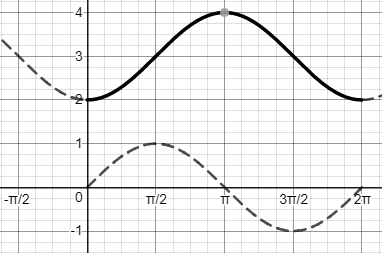
\includegraphics[width=8cm]{trigShift1}
\end{center}


\example Sketch $y =\cos  (x -\frac{\pi }{6})$.\medskip\\
\solution You could use a table of values however this is $y =\cos  x$ with a horizontal shift of $\frac{\pi }{6}$ to the right. Sketch the transformation on top of the graph of $y =\cos  x $.
\begin{center}
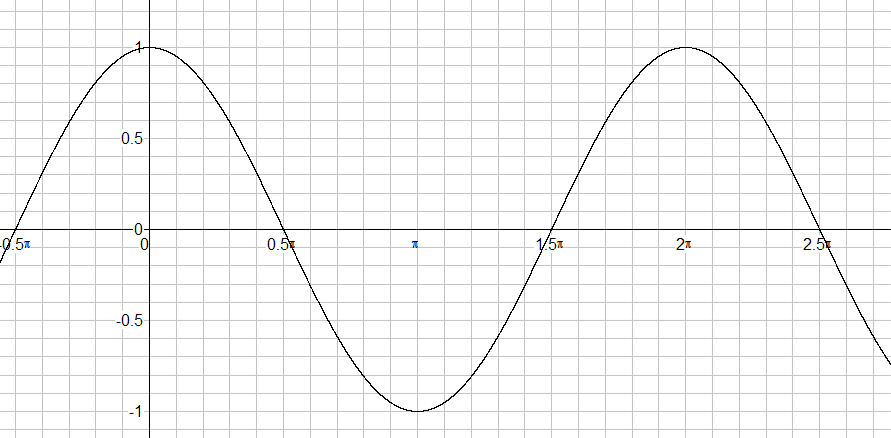
\includegraphics[width=10cm]{L4SZ270H}
\end{center}

In general $y =a \sin  x$ represents a vertical stretch of $y =\sin  x$ by $a$. If $a$ is negative the transformation can either be described as a negative stretch or (preferably) as a \emph{stretch}
of $\left \vert a\right \vert $ followed by a \emph{reflection} in the $x$-axis. Recall the reflection of $y =f \left (x\right )$ in the $x$-axis is $y = -f \left (x\right )$. The number $\left \vert a\right \vert $ is called the \emph{amplitude} for both $y =\sin  x$ and $y =\cos  x$ shown below. 

If $0 <a <1$ the fractional stretch causes the curve to shrink vertically. For instance the curve
$y =\sin  x$ has a maximum value of $1$ and a minimum value of $ -1$. the curve $y =\frac{1}{2} \sin  x$ has a maximum value of $\frac{1}{2}$ and a minimum value of $ -\frac{1}{2}$. 
\columnsep=10pt
\begin{multicols}{3}
\example  \medskip\\Sketch $y =\cos  ( -t)$\\ 
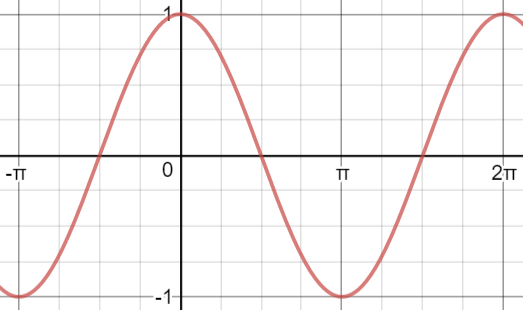
\includegraphics[width=5.5cm]{trigTrans1}

\columnbreak

\example \medskip\\Sketch $y =\sin \left( \frac{1}{2}x\right)$\\
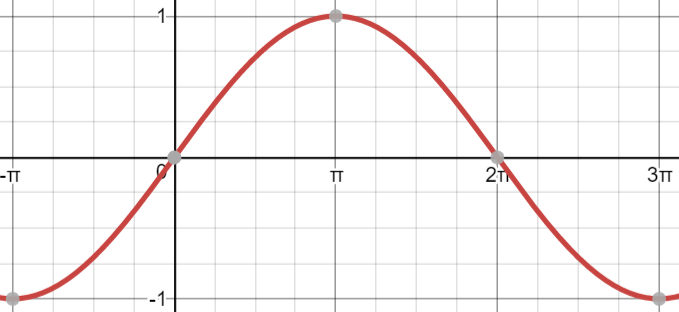
\includegraphics[width=5.5cm]{trigTrans2}
\columnbreak

\example \medskip\\Sketch $y =\cos(2x)$\\
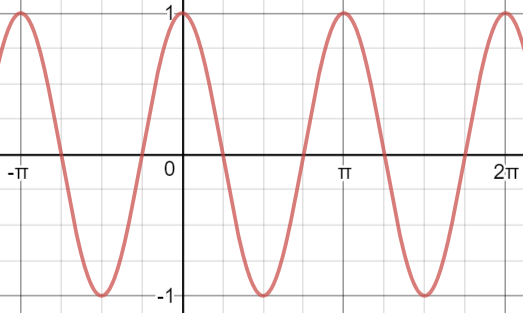
\includegraphics[width=5.5cm]{trigTrans3}
\end{multicols}

\subsection*{Tangent}
 There are other trig functions that we will not be covering here, for example the reciprocal functions are cosecant$=\frac{1}{\sin\theta}$, secant$=\frac{1}{\cos\theta}$, and the inverse tangent function, cotangent$=\frac{1}{\tan\theta}$. By focussing on sine, cosine and tangent the majority of problems we encounter can be solved. Tangent is the odd function out of the trio of common ones.

Previously we learnt that the period for the sine and cosine functions was $2 \pi $. Tangent is also a periodic function and it has a period of $\pi $ (not $2 \pi $). This means that it goes through one complete cycle every $\pi$. Recall $\tan  x =\frac{\sin  x}{\cos  x}$. To analyse the behaviour of the tangent function it helps if you know what you are looking for. Some key values of tangent will show the pattern. 
\begin{center}
\begin{tabular}{lrrrl}\toprule
	$x$  & $\qquad\sin  x$  & $\qquad\cos  x$  &\qquad& $\tan  x$  \\
	\midrule
	$ -\frac{\pi }{2}$  & $ -1$  & $0$  && $\frac{ -1}{0} = -\infty $  \\
	\midrule
	$ -\frac{\pi }{4}$  & $ -\frac{\sqrt{2}}{2}$  & $\frac{\sqrt{2}}{2}$  && $ -\frac{\sqrt{2}}{2} \div \frac{\sqrt{2}}{2} = -1$  \\
	\midrule
	$0$  & $0$  & $1$  && $\frac{0}{1} =0$  \\
	\midrule
	$\frac{\pi }{4}$  & $\frac{\sqrt{2}}{2}$  & $\frac{\sqrt{2}}{2}$  && $\frac{\sqrt{2}}{2} \div \frac{\sqrt{2}}{2} =1$  \\
	\midrule
	$\frac{\pi }{2}$  & $1$  & $0$  && $\frac{1}{0} =\infty $  \\
	\bottomrule
\end{tabular}
\end{center}


As $x$ takes values from $ -\frac{\pi }{2}$ to $\frac{\pi }{2}$, $\tan(x)$ takes values from $ -\infty $ to $\infty $. This pattern is repeated every $\pi $. 
A Desmos graph can show this relationship. The dashed lines are the asymptotes.
\begin{center}
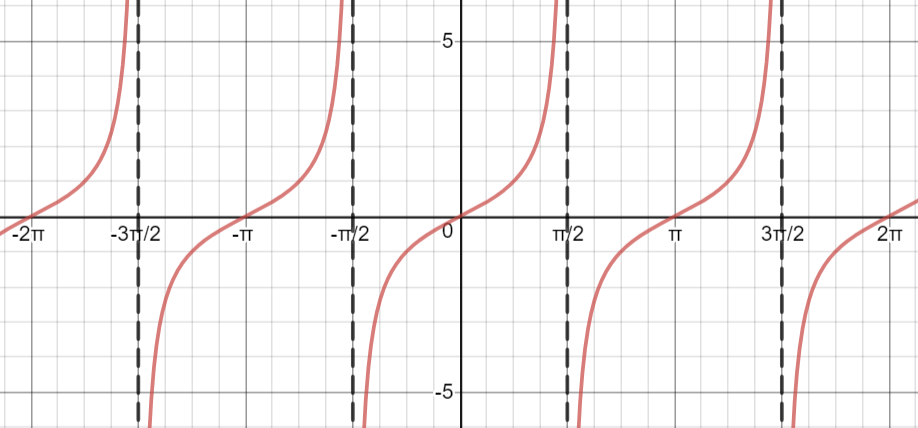
\includegraphics[width=12cm]{trigTan}\end{center}
The graph can be seen to have point symmetry. If you rotate the tangent curve through a half turn using the origin as axis the curve will lie on top of itself. This is a pictorial representation of an odd function.

Aside: You must not confuse $y =\tan  x$ with $y =x^{3}$. While they may appear to be similar in shape the only similarities are that they both pass through the origin and continue towards $\infty $ in the first quadrant and $ -\infty $ in the third quadrant. 

%---------------------------------------------------
% sine rule and cosing rule
%---------------------------------------------------
\section{Applications}\label{sec:applications}
\subsection*{The Sine Rule}
The Sine Rule is a relationship that allows you to find the sides and angles in triangles \textit{without} a right angle. In the next section we use the Cosine Rule to find sides and angles in triangles also, so as you study these two sections you need to learn which problems require the Sine Rule and which require the Cosine Rule. Previously, we met the formula for the area of a triangle given two sides and the included angle $\left ( \text{area}=\frac{1}{2} a b \sin  C\right )$. The Sine Rule and Cosine Rule also require specific combinations of sides and angles. Using standard side and angle labelling for a triangle $\rightarrow$ $\Delta A B C$ and let the sides be $a$, $b$ and $c$ where $a$ is opposite $\angle A$ etc. 
\begin{center}

\includegraphics[width=6cm]{L4SZ281W}
\end{center}
\begin{tcolorbox}
	The Sine Rule states that in any triangle
	\begin{equation*}\frac{\sin  A}{a} =\frac{\sin  B}{b} =\frac{\sin  C}{c}\qquad%
	\text{ or, inversely as: }%
	\qquad\frac{a}{\sin  A} =\frac{b}{\sin  B} =\frac{c}{\sin  C}
	\end{equation*}\end{tcolorbox}
Textbooks may use the term ``The Law of Sines" whereas in these notes the term ``The Sine Rule will be used. 


\subsection*{Proof of the Sine Rule}
The Sine Rule is easy to prove from the formula for the area of a triangle
\begin{equation*}\text{Area} =\frac{1}{2} b c \sin  A =\frac{1}{2} a c \sin  B =\frac{1}{2} a b \sin  C
\end{equation*}

Multiply right through by 2
\begin{equation*}b c \sin  A =a c \sin  B =a b \sin  C
\end{equation*}

Divide right through by $a b c$
\begin{equation*}\frac{\sin  A}{a} =\frac{\sin  B}{b} =\frac{\sin  C}{c}
\end{equation*}

\begin{multicols}{2}
\example Find side lengths $a$ and $c$ in the following triangle.

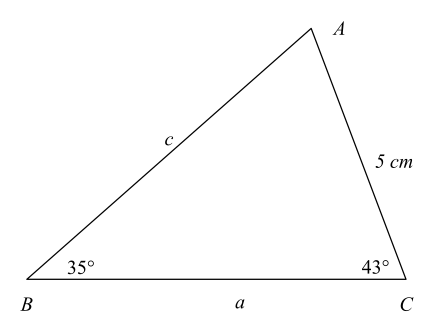
\includegraphics[ width=2.6143in, height=2.0159in,]{L4SZ281X}

\columnbreak
\solution \medskip\\(a) To find $c$
\begin{align*}\frac{c}{\sin  C} &  = \frac{b}{\sin  B} \\
\frac{c}{\sin  43 } &  = \frac{5}{\sin  35 } \\
c &  = \frac{5 \sin  43 }{\sin  35 } \\
&  \approx   5.95 \mbox{cm}\text{(2 dp)}\end{align*} \\

(b) To find $a$ 
(i) $A =\ang{180}  -(\ang{35}  +\ang{43} ) =\ang{180}  -\ang{78}  =\ang{102} $ 
(ii) It is usually wise to go back to the original data (i.e. use $b$ and $B$ rather than $c$ and $C$).
\begin{align*}\frac{a}{\sin  A} &  = \frac{b}{\sin  B} \\
\frac{a}{\sin  102 } &  = \frac{5}{\sin  35 } \\
a &  = \frac{5 \sin  102 }{\sin  35 } \\
&  \approx   8.53 \mbox{cm}\text{(2 dp)}\end{align*}\end{multicols}

These two calculations illustrate the first two cases in which the Sine Rule is used. You will notice that the triangle has been completely solved in the course of this example. We started with one side and two angles and we found the other two sides and the other angle. 

The third case is not as straight forward. Given two sides and an angle there could be no triangle formed, one triangle formed or two triangles formed depending on the length of the side opposite the given angle. You should develop an insight into the reasons why this is so. Imagine the second side given is the boom of a crane and the angle given is the angle between the boom and the ground. The side opposite the given angle is represented by the cable. It is clear that for certain lengths of the cable the hook will not reach the ground. Then as the hook is lowered a point will be reached when the hook just touches the ground.  

\columnsep =30pt
\begin {multicols}{2}

\includegraphics[ width=2.9577in, height=2.2061in,]{L4SZ281Y}

It is no surprise that the length $a$ to create this situation is $a =b \sin  A\text{.}$ 

We are after all dealing with the Sine Rule which becomes the fundamental sine formula $\left (\sin  A =\frac{\text{opp}}{\text{hyp}} =\frac{a}{b}\right )$ when the triangle has a right angle. 
\end {multicols}

If the cable is held taut and is extended a little more it will touch the ground in two places (provided it is kept in the same plane). As the cable is extended further the time will come where the cable is as long as boom. At this point there is only one solution again, the one straight out in front of the crane). Further extensions of the cable will produce only one solution (straight out in front of the crane) as the cable will theoretically reach behind the crane boom thus creating a different triangle altogether. 

The two solutions case is often referred to as the ambiguous case. The discussion above shows the range of values of $a$ that will give two solutions.
\begin{equation*}b \sin  A <a <b
\end{equation*}

\example Given $a =\ang{30} $, $a =8$ and $b =7$ solve the triangle (i.e. find $B$, $C$ and $c$). \\
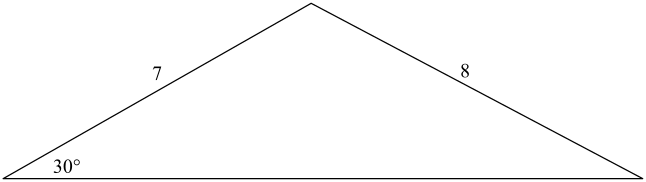
\includegraphics[ width=4.2739in, height=1.2202in,]{L4SZ281Z}\\
Because $8 >7$ this is the one solution case. \\
\solution
\begin{tasks}[counter-format=(tsk[1]),before-skip = {0ex},after-skip={-5ex}](3)
\task Find $B$
\begin{align*}\frac{\sin  B}{b} &  = \frac{\sin  A}{a} \\
\sin  B &  = \frac{b \sin  A}{a} \\
&  = \frac{7 \sin  30 }{8} =0.4375 \\
B &  = \sin ^{ -1} 0.4375 \approx \ang{25.94} \end{align*}

\task Find $C$
\begin{align*}C &  = \ang{180}  -(\ang{30}  +\ang{25.94} ) \\
&  = \ang{124.06} \end{align*}

\task Find $c$
\begin{align*}\frac{c}{\sin  C} &  = \frac{a}{\sin  A} \\
c &  = \frac{a \sin  C}{\sin a} \\
&  = \frac{8 \sin  124.06 }{\sin  30 } \\
&  \approx   13.3\end{align*}
\end{tasks}
%--------ambiguous case example---------------------------
\example {The Ambiguous Case} \\
Given $A =\ang{30} $, $a =6$ and $b =7$ solve the triangle. 

\solution In this case $b \sin  A =3.5$ and $b =7$ so as $a$ lies between $3.5$ and $7$. This is the ambiguous case, therefore there are two solutions as the side lengths and angle can product two different trianges.
\columnsep =30pt
\begin {multicols}{2}
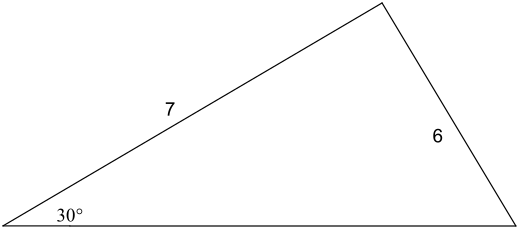
\includegraphics[ width=2.8885in, height=1.2825in,]{L4SZ2820}
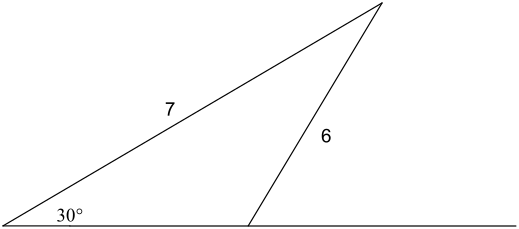
\includegraphics[ width=2.9308in, height=1.3015in,]{L4SZ2821}
\end {multicols}
It is best to visualise these two solutions on the same diagram so that the isosceles triangle can help lead to the two results. 
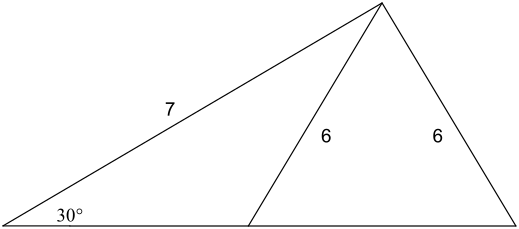
\includegraphics[ width=2.9585in, height=1.3136in,]{L4SZ2822}

\textbf{First solution} (Proceed as before) 
\begin{tasks}[counter-format=(tsk[1]),before-skip = {0ex},after-skip={-5ex}](3)
	\task Find $B$
\begin{align*}\frac{\sin  B}{b} &  = \frac{\sin  A}{a} \\
\sin  B &  = \frac{b \sin  A}{a} \\
&  = \frac{7 \sin  30 }{6} =0.58 \dot{3} \\
B &  = \sin ^{ -1} 0.58 \dot{3} \approx \ang{35.69} \end{align*}

\task Find $C$
\begin{align*}C &  = \ang{180}  -(\ang{30}  +\ang{35.69} ) \\
&  = \ang{114.31} \end{align*}

\task Find $c$
\begin{align*}\frac{c}{\sin  C} &  = \frac{a}{\sin  A} \\
c &  = \frac{a \sin  C}{\sin  A} \\
&  = \frac{6 \sin  114.31 }{\sin  30 } \\
&  \approx   10.9\end{align*}
\end{tasks}
\textbf{Second solution} 
\begin{tasks}[counter-format=(tsk[1]),before-skip = {0ex},after-skip={-5ex}](2)
	\task Find the second value of $B$ \\
$B =\ang{180}  -\ang{35.69}  =\ang{144.31} $
\task Find $C$\\
$C =\ang{180} -(\ang{30}  +\ang{144.31} ) =\ang{180}  -\ang{174.31}  =\ang{5.69} $
\task*[](Or if you remember the rule that the exterior angle of a triangle is the sum of the two interior
opposite angles $C +\ang{30}  =\ang{35.69} $ so $C =\ang{35.69}  -\ang{30}  =\ang{5.69} $) 
\task*[(3)] Find $c$
\begin{align*}\frac{c}{\sin  C} &  = \frac{a}{\sin  A} \\
c &  = \frac{a \sin  C}{\sin  A} \\
&  = \frac{6 \sin  5.69 }{\sin  30 } \\
&  \approx   1.2\end{align*}
\end{tasks}

\subsection*{The Cosine Rule}
In this section we will state and prove the Cosine Rule (which is called "The Law of Cosines" in the textbook). The proof is given here for completeness. You will not be tested on your ability to reproduce it. The section will give examples where the Cosine Rule is used to solve problems using the \emph{triangle of vectors} and we will include revision of \emph{bearings} and the use of trigonometry in \emph{navigation}. 

\begin{tcolorbox}
	For any triangle side sides $a$, $b$, and $c$ and angle $A$ opposite side $a$:\\
	\begin{center}
		$a^{2} =b^{2} +c^{2} -2 b c \cos  A$
	\end{center}	
\end{tcolorbox}

\subsection*{Proof of The Cosine Rule}
\textbf{To prove:} For any triangle $ \Delta A B C\text{,}$ $a^{2} =b^{2} +c^{2} -2 b c \cos  A$ \\ 
\columnsep =30pt
\begin {multicols}{2}
\setlength\fboxrule{0in}\setlength\fboxsep{0.2in}\fcolorbox[HTML]{000000}{FFFFFF}{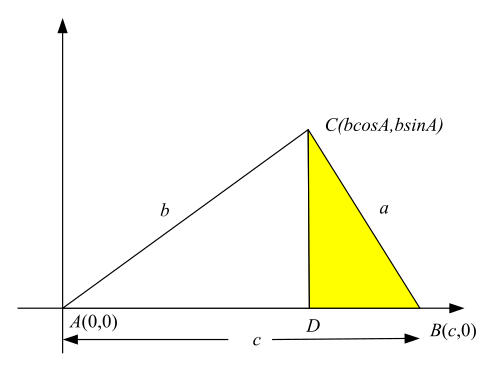
\includegraphics[ width=3.1021in, height=2.3549in,]{L4SZ282A}}
By Pythagoras' Theorem
\begin{align*}B C^{2} &  = C D^{2} +D B^{2} \\
a^{2} &  = \left (c -b \cos  A\right )^{2} +\left (b \sin  A\right )^{2} \\
&  = c^{2} -2 b c \cos  A +b^{2} \cos ^{2} A +b^{2} \sin ^{2} A \\
&  = c^{2} -2 b c \cos  A +b^{2} \left (\cos ^{2} A +\sin ^{2} A\right ) \\
&  = c^{2} -2 b c \cos  A +b^{2}\text{as}\cos ^{2} A +\sin ^{2} A =1\text{\ }\end{align*} 
\end {multicols}
This is usually written
\begin{equation*}a^{2} =b^{2} +c^{2} -2 b c \cos  A
\end{equation*}

The diagram has been drawn to simplify the way the proof unfolds. You will see that by placing the vertex $A$ at the origin the side $a$ is found in terms of $b$, $c$, and $A$. The proof would have been the same had $A$ and $B$ been as shown and $C$ placed in the second quadrant. (Thus producing a triangle with an obtuse angle at $A$.) This rule is symmetrical. You need to be given two sides and the included angle ($b$, $c$ and $A$) and the formula allows you to calculate $a$. Most textbooks will therefore show you three equivalent formulae
\begin{align*}a^{2} &  = b^{2} +c^{2} -2 b c \cos  A \\
b^{2} &  = c^{2} +a^{2} -2 c a \cos  B \\
c^{2} &  = a^{2} +b^{2} -2 a b \cos  C\end{align*}

\example Given $a =5$, $b =6$ and $C =\ang{50} $, find $c$.\medskip\\
\solution
\begin{align*}c^{2} &  = a^{2} +b^{2} -2 a b \cos  C \\
&  = 5^{2} +6^{2} -2 \times 5 \times 6 \times \cos  50  \\
&  \approx   22.43274342 \\
c &  \approx   \sqrt{22.43274342} \\
&  \approx   4.736321718 \approx 4.7 \left (1\text{dp}\right )\end{align*}
\rule{6.8cm}{0.5pt}\\
\example Given $a =5$, $b =6$ and $C =\ang{130} $, find $c$.\medskip\\
\solution
\begin{align*}c^{2} &  = a^{2} +b^{2} -2 a b \cos  C \\
&  = 5^{2} +6^{2} -2 \times 5 \times 6 \times \cos  130  \\
&  \approx   99.56725658 \\
c &  \approx   \sqrt{99.56725658} \\
&  \approx   9.97833937 \approx 10.0 \left (1\text{dp}\right )\end{align*}

These two examples show that when the two sides and the included angle are given the third side
(opposite the given angle) can be found. 

\example Find the angle given three side lengths; given $a =5$, $b =6$ and $c =9$, find $A$. \medskip\\
\solution Because $a$ is the smallest side $A$ will most certainly be an acute angle.
\begin{align*}\cos  A &  = \frac{b^{2} +c^{2} -a^{2}}{2 b c} \\
&  = \frac{6^{2} +9^{2} -5^{2}}{2 \times 6 \times 9} \\
&  \approx 0.851851851 \\
A &  \approx \cos ^{ -1} \left (0.851851851\right ) \\
&  \approx \ang{31.6} 
\end{align*}

%---------------------------------------------------
% Chapter Exercises in a separate file
%---------------------------------------------------
\section{Chapter Exercises}
\subimport{}{TrigExercises}


%---------------------------------------------------
% Exponential Functions
%---------------------------------------------------
\chapter{Exponential Functions}

We defined $a^{x}$ where $a >0$ in chapter 1, however $x$ was restricted to rational numbers. We now want to explore $a^{x}$ where $a >0$ and $x$ is any real number. 

We can show that values exist simply by pressing buttons on the calculator or drawing
a graph using Desmos, however an intuitive understanding can be obtained by considering appropriate values. 

Consider $2^{\pi }$. We know $\pi  =3.141592654 \ldots $. $2^{\pi }$ should be between $2^{3}$\ and $2^{4}$. That is between $8$ and $16$. We can evaluate 

\qquad \qquad \qquad \qquad \qquad \qquad \qquad \qquad
\begin{tabular}[c]{ll}$2^{3.1}$  & $8.5741877$  \\
$2^{3.14}$  & $8.815240927$  \\
$2^{3.141}$  & $8.821353305$  \\
$2^{3.1415}$  & $8.824411082$  \\
$2^{3.14159}$  & $8.824961595$  \\
$2^{3.141592}$  & $8.824973829$  \\
$2^{3.1415926}$  & $8.824977499$  \\
$2^{3.14159265}$  & $8.824977805$  \\
$2^{3.141592654}$  & $8.82497783$
\end{tabular}

We could continue this process. If
we enter $2^{\pi }$ on the calculator the answer obtained is
\begin{equation*}2^{\pi } =8.824977827
\end{equation*}

The graph of $y =2^{x}$, $ \forall x \in \mathbb{R}$ is shown. 
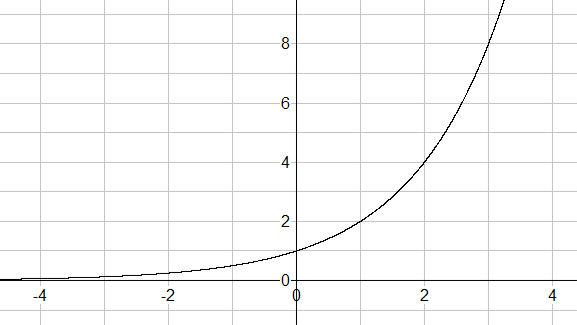
\includegraphics[width=3.7758in, height=2.1378in,]{L4SZ282M}

Recall $y =f (x)$ is a function and $y =f ( -x)$ is the same function with every $x$ replaced with $ -x$, i.e. $y =f ( -x)$ is the reflection of $y =f (x)$ in the $y$-axis. 

If $y =2^{x}$ then $y =2^{ -x}$ is the reflection of $y =2^{x}$ in the $y$-axis. But $y =2^{ -x} =\left (2^{ -1}\right )^{x} =\genfrac{(}{)}{}{}{1}{2}^{x}$. 

\subsubsection{Graphing Exercise}
Use Desmos to verify that $y =2^{ -x}$ and $y =\genfrac{(}{)}{}{}{1}{2}^{x}$ are the same. 

%Here are the graphs of $y =2^{x}$ and $y =2^{ -x}$. 

   
%\setlength\fboxrule{0.01in}\setlength\fboxsep{0.2in}\fcolorbox[HTML]{000000}{FFFFFF}{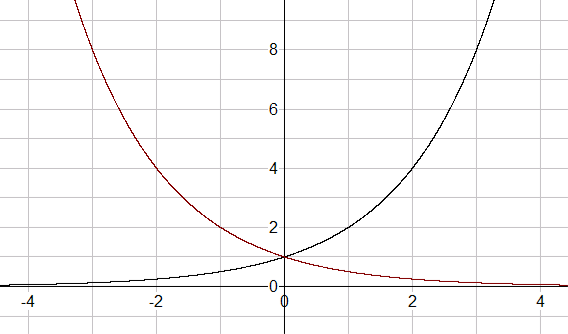
\includegraphics[ width=3.7265in, height=2.2027in,]{L4SZ282N}
%}


\subsection{The Exponential Function $f (x) =a^{x}$}
Let $y =a^{x}$ where $a >0$ 


\begin{tabular}[c]{|l|c|l|}\hline
When $0 <a <1$  & $y =a^{x}$ looks like  &    
\setlength\fboxrule{0in}\setlength\fboxsep{0.2in}\fcolorbox[HTML]{000000}{FFFFFF}{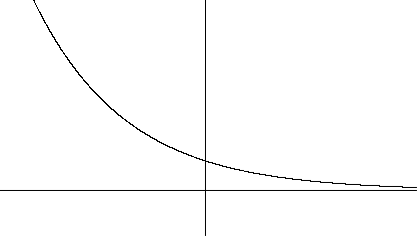
\includegraphics[ width=1.9086in, height=1.0853in,]{L4SZ282O}
}
\\
\hline
When $a =1$  & $y =a^{x} =1^{x} =1$ looks like  &    
\setlength\fboxrule{0in}\setlength\fboxsep{0.2in}\fcolorbox[HTML]{000000}{FFFFFF}{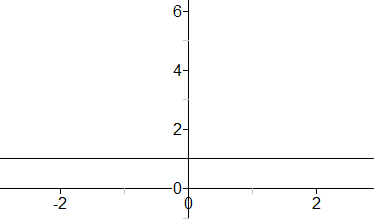
\includegraphics[ width=1.9095in, height=1.1234in,]{L4SZ282P}
}
\\
\hline
When $a >1$  & $y =a^{x}$ looks like  &    
\setlength\fboxrule{0in}\setlength\fboxsep{0.2in}\fcolorbox[HTML]{000000}{FFFFFF}{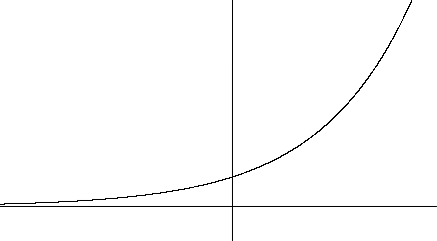
\includegraphics[ width=1.9372in, height=1.0741in,]{L4SZ282Q}
}
\\
\hline
\end{tabular}

$f (x) =a^{x}$ is called an \emph{exponential} function. $a$ is called the \emph{base} of the exponential function. The domain
is $\mathbb{R}$. the range is $\left (0 ,\infty \right )$. The $x$-axis is an asymptote. 

\subsubsection{Example 1}
Find the equation of the exponential function that passes through $\left (0 ,1\right )$ and $\left (3 ,125\right )$. 

Solution: An
exponential function that passes through $\left (0 ,1\right )$ is of the form $f (x) =a^{x}$. As $f (3) =125$ we substitute $x =3$ and get
\begin{align*}a^{3} &  = 125 \\
a &  = \sqrt[{3}]{125} =5\end{align*}

\subsection{Transformations of Exponential Functions}
Recall the transformations we have met so far 


\begin{tabular}[c]{ll}Vertical stretch of $a$  & $y =f (x) \leadsto y =a f (x)$  \\
Horizontal stretch of $\frac{1}{b}$  & $y =f (x) \leadsto y =f (b x)$  \\
Vertical shift of $c$ $\uparrow $  & $y =f (x) \leadsto y =f (x) +c$  \\
Horizontal shift of $d$ $ \longrightarrow $  & $y =f (x) \leadsto y =f (x -d)$  \\
Reflection in $x$-axis  & $y =f (x) \leadsto y = -f (x)$  \\
Reflection in $y$-axis  & $y =f (x) \leadsto y =f ( -x)$
\end{tabular}

Each of these transformations can be applied to an exponential
function. 

Given $y =2^{x}$ apply the following transformations. Draw a sketch showing where the graph crosses the
$y$-axis, its shape, its asymptote and one other point it passes through. 


\columnseprule =0.4pt
\begin {multicols}{2}

\begin{enumerate}
\item Horizontal shift of $ +2\vspace{+2.000000cm}$ 

\item Vertical shift of $ -3\vspace{+2.000000cm}$ 

\item Horizontal stretch of $2\vspace{+2.000000cm}$ 

\item Vertical stretch of $4\vspace{+2.000000cm}$ 

\item Horizontal stretch of $\frac{1}{3}\vspace{+2.000000cm}$ 

\item Vertical stretch of $\frac{1}{2}\vspace{+2.000000cm}$ 

\item Reflection in the x-axis\vspace{2cm}


\item Reflection in the y-axis\vspace{2cm} 

\item (Challenge) Reflection in $y = -1\vspace{+2.000000cm}$ 

\item (Challenge) Reflection in $x =1\vspace{+2.000000cm}$ \end{enumerate}

\end {multicols}


%---------------------------------------------------
% the natural exponential function e^x
%---------------------------------------------------
\section{\ensuremath{e^x}}

The \emph{natural exponential function} has wide application in mathematics and is a particular example of the exponential
function. We have defined $f (x) =a^{x}$ and there is a particular value of $a$ that we denote by the letter $e$. This will turn up again and again in future courses and later it will be carefully
defined for you. In this course we will meet some of the applications that use $e$. $e$ is an irrational number (like $\pi $, $\sqrt{2}$ etc.). It can be found on the calculator and to 20 decimal places it is
\begin{equation*}e \approx 2.71828182845904523536
\end{equation*}

The natural exponential function $f (x) =e^{x}$ is often simply referred to as the exponential function. 

\subsubsection{Example 2}
Use your calculator to evaluate to 5dp 


\begin{description}
\item [(a)] $e^{4}$ 

\item [(b)] $2 e^{ -0.7}$ 

\item [(c)] $e^{3.1}$ 

\item [(d)] $e^{e}$ \end{description}

($54.59815$, $0.99317$, $22.19795$, $15.15426$) 

\subsection{Exercise 1}
Use Desmos to sketch: 

\begin{description}
\item [(a)] $f (x) =e^{ -x}$ 

\item [(b)] $g (x) =2 e^{0.1 x}$ 

\item [(c)] $h (x) = -2.1 e^{ -0.12 x}$ \end{description}

\subsection{Exercise 2}
The exponential function can be used to model the way populations grow and diseases spread. The following
example is about the spread of an infectious disease in a small city whose population is $10,000$. After $t$ days the number of people who have caught the disease is modelled by the function
\begin{equation*}f (t) =\frac{10000}{5 +2495 e^{ -0.84 t}}
\end{equation*}


\begin{description}
\item [(a)] How many people had the disease initially? 

\item [(b)]
How many people have the disease after $1$ day? 

\item [(c)] How many people
have the disease after $5$ days? 

\item [(d)] Use Desmos
to graph the function. 

\item [(e)] Describe the behaviour
of the function. \end{description}

The graph has distinctive characteristics. It
starts at a particular nonzero value (when $t =0$) and increases slowly at first then more rapidly. It slows down after a time and
levels off because the exponential function in the denominator $ \leadsto 0$ when $t \leadsto \infty $. Graphs with these characteristics are called logistic curves. The
particular model is called a logistic growth model. 

\subsection{Exercises}
Find the exponential function $f (x) =a^{x}$ whose graph is given. 


\begin{tabular}[c]{ll}9.  & 10.
\\
   
\setlength\fboxrule{0.01in}\setlength\fboxsep{0.2in}\fcolorbox[HTML]{000000}{FFFFFF}{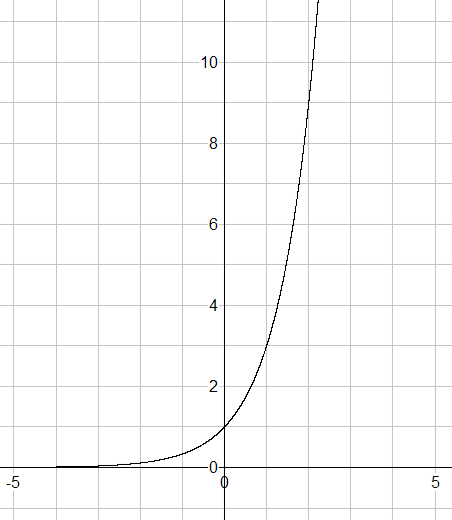
\includegraphics[ width=2.3047in, height=2.6472in,]{L4SZ282R}
}
&    
\setlength\fboxrule{0.01in}\setlength\fboxsep{0.2in}\fcolorbox[HTML]{000000}{FFFFFF}{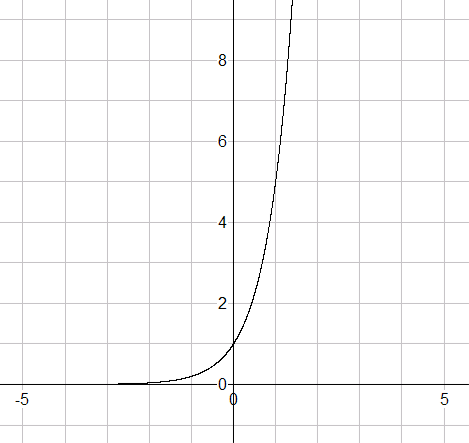
\includegraphics[ width=2.7164in, height=2.5676in,]{L4SZ282S}
}
\\
11.  & 12.  \\
\setlength\fboxrule{0.01in}\setlength\fboxsep{0.2in}\fcolorbox[HTML]{000000}{FFFFFF}{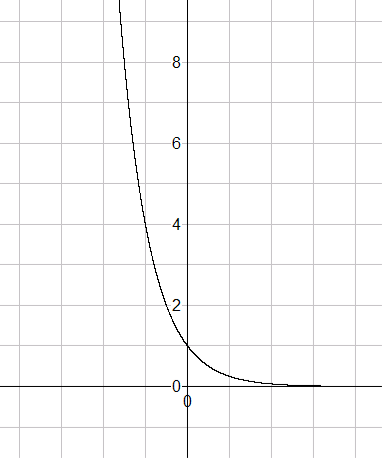
\includegraphics[ width=2.207in, height=2.6394in,]{L4SZ282T}
}
&    
\setlength\fboxrule{0.01in}\setlength\fboxsep{0.2in}\fcolorbox[HTML]{000000}{FFFFFF}{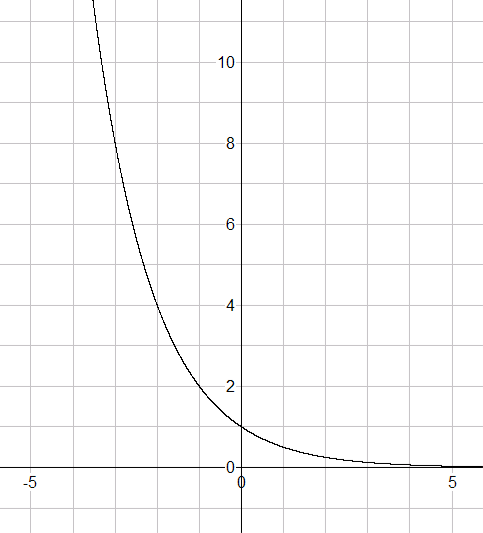
\includegraphics[ width=2.3938in, height=2.6385in,]{L4SZ282U}
}
\end{tabular}

For the following questions draw the graph of the function by transforming the given graph. State the domain, range and asymptote.  

\begin{tabular}[c]{ll}19. The given graph is $y =3^{x}\text{.}$ Draw $y = -3^{x}\vspace{+0.200000cm}$  & 21. The given graph is $y =2^{x}\text{.}$\ Draw $y =2^{x} -3$  \\
   
\setlength\fboxrule{0.01in}\setlength\fboxsep{0.2in}\fcolorbox[HTML]{000000}{FFFFFF}{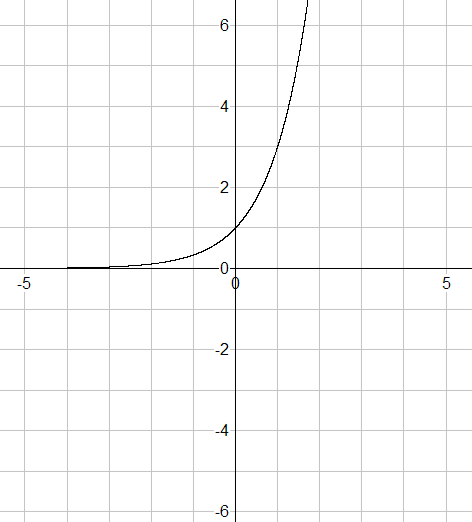
\includegraphics[ width=2.1594in, height=2.1851in,]{L4SZ282V}
}
\vspace*{0.5cm}  &    
\setlength\fboxrule{0.01in}\setlength\fboxsep{0.2in}\fcolorbox[HTML]{000000}{FFFFFF}{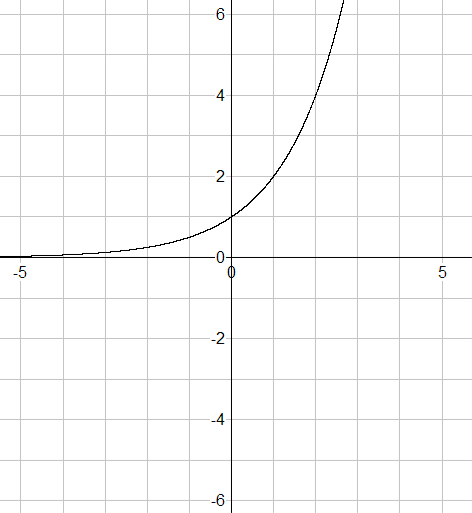
\includegraphics[ width=2.1793in, height=2.1679in,]{L4SZ282W}
}
\\
23. The given graph is $y =\frac{1}{2}^{x}\text{.}$ Draw $y =4 +\frac{1}{2}^{x}\vspace{+0.200000cm}$  & 25. The given graph is $y =10^{x}\text{.}$ Draw $y =10^{x +3}$  \\
   
\setlength\fboxrule{0.01in}\setlength\fboxsep{0.2in}\fcolorbox[HTML]{000000}{FFFFFF}{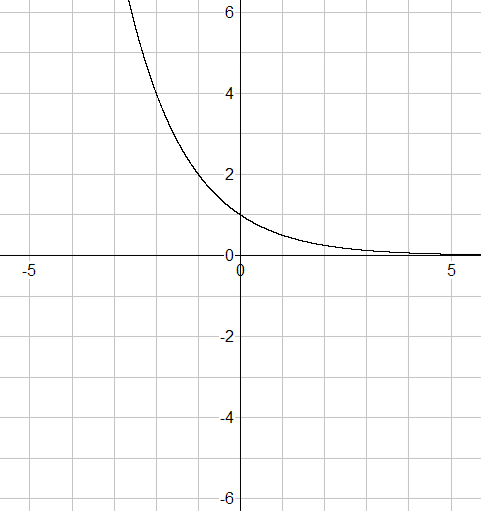
\includegraphics[ width=2.271in, height=2.2111in,]{L4SZ282X}
}
\vspace*{0.5cm}  &    
\setlength\fboxrule{0.01in}\setlength\fboxsep{0.2in}\fcolorbox[HTML]{000000}{FFFFFF}{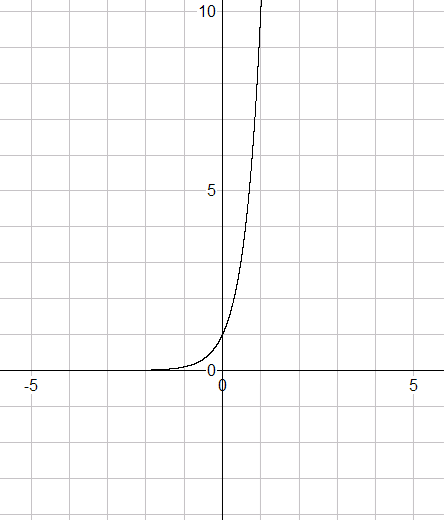
\includegraphics[ width=2.0496in, height=2.1964in,]{L4SZ282Y}
}
\\
27. The given graph is $y =e^{x}\text{.}$ Draw $y = -e^{x}\vspace{+0.200000cm}$  & 29. The given graph is $y =e^{ -x}\text{.}$ Draw $y =e^{ -x} -1$  \\
   
\setlength\fboxrule{0.01in}\setlength\fboxsep{0.2in}\fcolorbox[HTML]{000000}{FFFFFF}{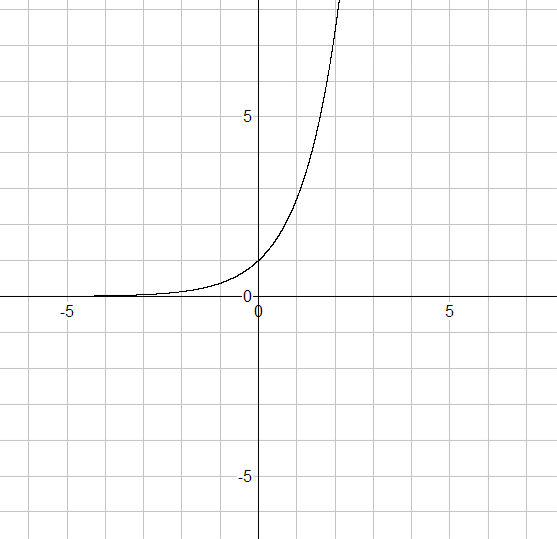
\includegraphics[ width=2.5114in, height=2.1319in,]{L4SZ282Z}
}
&    
\setlength\fboxrule{0.01in}\setlength\fboxsep{0.2in}\fcolorbox[HTML]{000000}{FFFFFF}{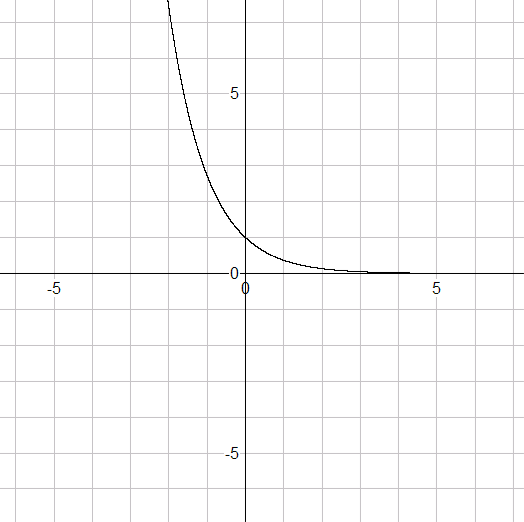
\includegraphics[ width=2.4336in, height=2.1241in,]{L4SZ2830}
}
\end{tabular} 


\begin{tabular}[c]{ll}31. The given graph is $y =e^{x}\text{.}$Draw $y =e^{x -2}$  &  \\
   
\setlength\fboxrule{0.01in}\setlength\fboxsep{0.2in}\fcolorbox[HTML]{000000}{FFFFFF}{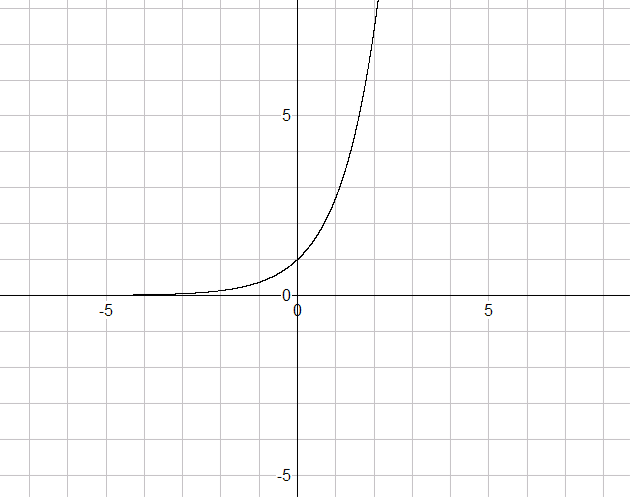
\includegraphics[ width=3.109in, height=2.4587in,]{L4SZ2831}
}
& 
\end{tabular}


\begin{description}
\item [43.] A radioactive substance decays in such a way that the amount
of mass remaining after $t$ days is given by the function
\begin{equation*}m (t) =13 e^{ -0.015 t}
\end{equation*} \\\relax Where $m (t)$ is measured in kilograms. 

\item [(a)]
Find the mass at time $t =0.$ 

\item [(b)] How much of the mass
remains after 45 days? 

\item [45.] A sky diver jumps from
a reasonable height above the ground. The air resistance she experiences is proportional to her velocity, and
the constant of proportionality is $0.2$. It can be shown that the downward velocity of the sky diver at time $t$ is given by
\begin{equation*}v (t) =80 \left (1 -e^{ -0.2 t}\right )
\end{equation*} \\\relax where $t$ is measured in seconds and $v (t)$ is measured in feet per second ($\mbox{ft}$/$\mbox{s}$). 

\item [(a)]
Find the initial velocity of the sky diver. 

\item [(b)] Find
the velocity after $5 \mbox{s}$ and after $10 \mbox{s}$. 

\item [(c)]
Draw a graph of the velocity function $v (t)\text{.}$ 

\item [(d)] The maximum
velocity of a falling object with wind resistance is called the \emph{terminal velocity}. From
the graph in part (c) find the terminal velocity of the sky diver. 

\item [48.]
The population of a certain species of bird is limited by the type of habitat required for nesting. The population
behaves according to the \emph{logistic growth model}
\begin{equation*}n (t) =\frac{5600}{0.5 +27.5 e^{ -0.044 t}}
\end{equation*} \\\relax where $t$ is measured in years. 

\item [(a)]
Find the initial bird population. 

\item [(b)] Draw a graph
of the function $n (t)\text{.}$ 

\item [(c)] What size does
the population approach as time goes on? \end{description}

 

\section{Logarithmic Functions}
The \emph{logarithmic function} is the inverse of the function $f (x) =a^{x}$. Recall the inverse of a function is the reflection of the function in the line $y =x$. Mathematically this is equivalent to swapping the $x$ and the y in $y =a^{x}$. So $x =a^{y}$ is the inverse of $y =a^{x}$. We have another notation for the inverse of a function, which is a little more complicated.
\ let $y =f (x)$ be a function of $x$ then $y =f^{ -1} (x)$ is the inverse of this function. Sometimes the inverse of the function is also a function.
\ For example the inverse of $y =x^{2}$ is $x =y^{2}$. $y =x^{2}$ is a function (vertical line test always applies), whereas $x =y^{2}$ is not a function (vertical line test is broken). 

   
\setlength\fboxrule{0.01in}\setlength\fboxsep{0.2in}\fcolorbox[HTML]{000000}{FFFFFF}{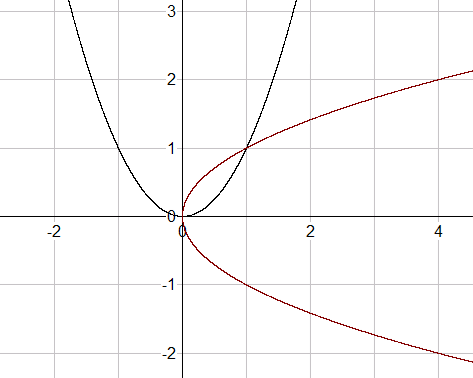
\includegraphics[ width=3.032in, height=2.4275in,]{L4SZ2832}
}


The inverse of $y =10^{x}$ is $x =10^{y}$. $y =10^{x}$ is a function (vertical line test always applies) and so is $x =10^{y}$. 

   
\setlength\fboxrule{0.01in}\setlength\fboxsep{0.2in}\fcolorbox[HTML]{000000}{FFFFFF}{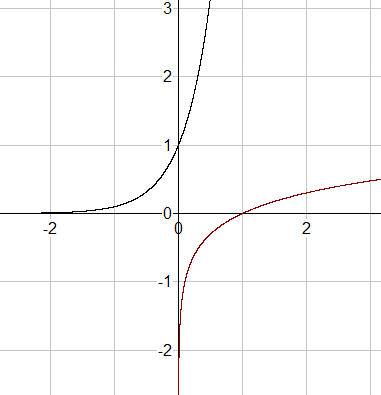
\includegraphics[ width=2.3419in, height=2.4267in,]{L4SZ2833}
}


Another useful fact to remember about inverses concerns the domain and range. The \emph{domain}
of $f$ is the \emph{range} of $f^{ -1}$ and the \emph{range} of $f$ is the \emph{domain} of $f^{ -1}$. 

We have a notation for $x =a^{y}$ it is $y =\log _{a} x$
\begin{equation}y =\log _{a} x \Leftrightarrow x =a^{y}\tag{1}
\end{equation}

In $x =a^{y}$ substitute $y =\log _{a} x$ and we get $x =a^{\log _{a} x}$. This means that given a base of $a$ the power (or exponent) to which $a$ must be raised to get $x$ is $\log _{a} x$. 

Problems involving logarithms will often require us to switch back and forth between $y =\log _{a} x$ and $x =a^{y}$, however it is also helpful if you can remember to substitute for $y$ and write $x =a^{\log _{a} x}$ so that you can say "the logarithm is the power". 

\subsubsection{Example 1}
\begin{description}
\item [(a)] $\log _{10} 100 =2$ because $10^{2} =100$ 

\item [(b)] $\log _{3} 81 =4$ because $3^{4} =81$ 

\item [(c)] $\log _{10} 0.01 = -2$ because $10^{ -2} =0.01$ \end{description}

\subsection{The graph of $y =\log _{a} x$}
The exponential function $y =a^{x}$ where $a >0$ is now known and its domain is $\mathbb{R}$ and its range is the positive real numbers. We often
write $\mathbb{R}^{ +}$ instead of $\left (0 ,\infty \right )$. 

The graph of $f (x) =a^{x}$ can be reflected in the line $y =x$ and the result is $f^{ -1} (x) =\log _{a} x$. 

\subsection{Graphing Exercise}


\subsubsection{Exercise 1}
On the same set of axes draw 


\begin{description}
\item [(a)] $y =10^{x}$ 

\item [(b)] $y =\log _{10} x$ 

\item [(c)] $y =x$ 

\item [(d)] $x =10^{y}$ \end{description}

Make a comment about each statement below. 

\begin{description}
\item [(1)] Check the graphs in (a), (b) and (c) are you confident that $y =\log _{10} x$ is the reflection of $y =10^{x}$ in the line $y =x$?\vspace{2cm} 

\item [(2)]
When you enter $x =10^{y}$ describe what takes place.\vspace{2cm} \end{description}

\subsubsection{Exercise 2}
On a \textbf{new} set of axes draw 


\begin{description}
\item [(a)] $y =2^{x}$ 

\item [(b)] $y =\log _{2} x$ \end{description}

There is no way to draw $y =\log _{2} x$ directly however (b) and (d) above gives you a way of doing it. 

\subsubsection{Exercise 3}
On a \textbf{new} set of axes draw 


\begin{description}
\item [(a)] $y =\log _{2} x$ 

\item [(b)] $y =\log _{3} x$ 

\item [(c)] $y =\log _{4} x$ 

\item [(d)] $y =\log _{5} x$ \end{description}

Notice the point that is common to all curves and the behaviour
of the family of curves for $x >1$ and for $0 <x <1$. 

\textbf{Property 1}: A property of logarithms is $\log _{a} 1 =0$ and this can be seen on the graphs where every graph goes through $\left (1 ,0\right )$. 

The pattern you observe as the base gets
bigger might not be evident for values of the base between $0$ and $1$. On the same set of axes draw the following: 


\begin{description}
\item [(e)] $y =\log _{\frac{1}{2}} x$ 

\item [(f)] $y =\log _{\frac{1}{3}} x$ 

\item [(g)] $y =\log _{\frac{1}{4}} x$ 

\item [(h)] $y =\log _{\frac{1}{5}} x$ \end{description}

To say the pattern is the same you have to be careful to describe
the base. Explain how changing the base gives the same pattern as for (a) to (d).


\textbf{Property 2:} A second property of logarithms is $\log _{a} a =1$. That is $a^{1} =a$ or the power to which you have to raise $a$ to get $a$ is $1$. On your curves above locate a point on each curve that shows this. You
should in each case be looking for the point $\left (a ,1\right )$. 

\textbf{Property 3:} A third property
of logarithms is $\log _{a} a^{x} =x$. This useful property must be understood if logarithm problems are to be mastered.
\ You should understand what $\log _{a} a^{x}$ is saying. $a$ is the base so $\log _{a} a^{x} =x$ says "The power to which $a$ must be raised to get $a^{x}$ is $x$." 

\subsection{Common Logarithms}
When the base is $10$ we write $y =\log _{10} x =\log  x$. If you see no base you assume it is base $10$. $y =\log  x$ is called the \emph{common} logarithm of $x$. Desmos and other programs with mathematics incorporated recognise "$\log $" as "logarithm to the base $10$". The $\log $ key on the calculator gives the common logarithm of any positive number.
\begin{equation*}y =\log  x \Leftrightarrow 10^{y} =x
\end{equation*}

\subsection{Natural Logarithms}
When the base is $e$ we write $y =\log _{e} x =\ln  x$. If you see $\ln  x$ you assume it is $\log _{e} x$. $y =\ln  x$ is called the \emph{natural} logarithm of $x$. Desmos and other programs with mathematics incorporated recognise "$\ln $" as "logarithm to the base $e$". The $\ln $ key on the calculator gives the natural logarithm of any positive number.
\begin{equation*}y =\ln  x \Leftrightarrow e^{y} =x
\end{equation*}

\subsection{Graphing Exercise}
Use Desmos to sketch the following. Describe in words how each curve is related to $y =\ln  x$. 


%TCIMACRO{\TeXButton{Begin 3 Columns}{\columnseprule =0pt
% \columnsep =30pt
% \begin {multicols}{3}}}%
%BeginExpansion
\columnseprule =0pt
\columnsep =30pt
\begin {multicols}{3}
%EndExpansion
 


\begin{description}
\item [(a)] $y =\ln  x$ 

\item [(b)] $y =\ln  ( -x)$ 

\item [(c)] $y = -\ln  x$ 

\item [(d)] $y =\ln  (x -1)$ 

\item [(e)] $y =\ln  (x) -1$ 

\item [(f)] $y =\ln  ( -1 -x)$ \end{description}


%TCIMACRO{\TeXButton{End 3 Columns}{\end {multicols}}}%
%BeginExpansion
\end {multicols}
%EndExpansion


\subsection{Exercises}
Express the equation in exponential form. 


\begin{tabular}[c]{lllllllllllll}1.  & (a)
& $\log _{5} 25 =2$  &  & (b)  & $\log _{5} 1 =0$  &  & 3.
& (a)  & $\log _{8} 2 =\frac{1}{3}$  &  & (b)  & $\log _{2} \genfrac{(}{)}{}{}{1}{8} = -3$  \\
5.  & (a)  & $\ln  5 =x$  &  & (b)  & $\ln  y =5$  &  &  &  &  &  &  & 
\end{tabular}

Express the equation in logarithmic form 


\begin{tabular}[c]{lllllllllllll}7.  & (a)
& $5^{3} =125$  &  & (b)  & $10^{ -4} =0.0001$  &  & 9.
& (a)  & $8^{ -1} =\frac{1}{8}$  &  & (b)  & $2^{ -3} =\frac{1}{8}$  \\
11.  & (a)  & $e^{x} =2$  &  & (b)  & $e^{3} =y$  &  &  &  &  &  &  & 
\end{tabular}

Evaluate the expression 


\begin{description}
\item [13. (a)]   
%TCIMACRO{\TeXButton{Begin 3 Columns}{\columnseprule =0pt
% \columnsep =30pt
% \begin {multicols}{3}}}%
%BeginExpansion
\columnseprule =0pt
\columnsep =30pt
\begin {multicols}{3}
%EndExpansion
 $\log _{3} 3$ 

\item [(b)] $\log _{3} 1$ 

\item [(c)] $\log _{3} 3^{2}$ 
%TCIMACRO{\TeXButton{End 3 Columns}{\end {multicols}}}%
%BeginExpansion
\end {multicols}
%EndExpansion
 

\item [15.
(a)]   
%TCIMACRO{\TeXButton{Begin 3 Columns}{\columnseprule =0pt
% \columnsep =30pt
% \begin {multicols}{3}}}%
%BeginExpansion
\columnseprule =0pt
\columnsep =30pt
\begin {multicols}{3}
%EndExpansion
 $\log _{6} 36$ 

\item [(b)] $\log _{9} 81$ 

\item [(c)] $\log _{7} 7^{10}$ 
%TCIMACRO{\TeXButton{End 3 Columns}{\end {multicols}}}%
%BeginExpansion
\end {multicols}
%EndExpansion
 

\item [17.
(a)]   
%TCIMACRO{\TeXButton{Begin 3 Columns}{\columnseprule =0pt
% \columnsep =30pt
% \begin {multicols}{3}}}%
%BeginExpansion
\columnseprule =0pt
\columnsep =30pt
\begin {multicols}{3}
%EndExpansion
 $\log _{3} \genfrac{(}{)}{}{}{1}{27}$ 

\item [(b)] $\log _{10} \sqrt{10}$ 

\item [(c)] $\log _{5} 0.2$ 
%TCIMACRO{\TeXButton{End 3 Columns}{\end {multicols}}}%
%BeginExpansion
\end {multicols}
%EndExpansion
 

\item [19.
(a)]   
%TCIMACRO{\TeXButton{Begin 3 Columns}{\columnseprule =0pt
% \columnsep =30pt
% \begin {multicols}{3}}}%
%BeginExpansion
\columnseprule =0pt
\columnsep =30pt
\begin {multicols}{3}
%EndExpansion
 $2^{\log _{2} 37}$ 

\item [(b)] $3^{\log _{3} 8}$ 

\item [(c)] $e^{\ln  \sqrt{5}}$ 
%TCIMACRO{\TeXButton{End 3 Columns}{\end {multicols}}}%
%BeginExpansion
\end {multicols}
%EndExpansion
 

\item [21.
(a)]   
%TCIMACRO{\TeXButton{Begin 3 Columns}{\columnseprule =0pt
% \columnsep =30pt
% \begin {multicols}{3}}}%
%BeginExpansion
\columnseprule =0pt
\columnsep =30pt
\begin {multicols}{3}
%EndExpansion
 $\log _{8} 0.25$ 

\item [(b)] $\ln  e^{4}$ 

\item [(c)] $\ln  \left (1/e\right )$ 
%TCIMACRO{\TeXButton{End 3 Columns}{\end {multicols}}}%
%BeginExpansion
\end {multicols}
%EndExpansion
 \end{description}

Use the definition of the logarithmic function to find $x$. 


\begin{description}
\item [23. (a)]   
%TCIMACRO{\TeXButton{Begin 4 Columns}{\columnseprule =0pt
% \columnsep =30pt
% \begin {multicols}{4}}}%
%BeginExpansion
\columnseprule =0pt
\columnsep =30pt
\begin {multicols}{4}
%EndExpansion
 $\log _{2} x =5$ 

\item [(b)] $\log _{2} 16 =x$ 

\item [25. (a)] $\log _{3} 243 =x$ 

\item [(b)] $\log _{3} x =3$ 
%TCIMACRO{\TeXButton{End 4 Columns}{\end {multicols}}}%
%BeginExpansion
\end {multicols}
%EndExpansion
 

\item [27.
(a)]   
%TCIMACRO{\TeXButton{Begin 4 Columns}{\columnseprule =0pt
% \columnsep =30pt
% \begin {multicols}{4}}}%
%BeginExpansion
\columnseprule =0pt
\columnsep =30pt
\begin {multicols}{4}
%EndExpansion
 $\log _{10} x =2$ 

\item [(b)] $\log _{5} x =2$ 

\item [29. (a)] $\log _{x} 16 =4$ 

\item [(b)] $\log _{x} 8 =\frac{3}{2}$ 
%TCIMACRO{\TeXButton{End 4 Columns}{\end {multicols}}}%
%BeginExpansion
\end {multicols}
%EndExpansion
 \end{description}

Find the domain of the function. 

\columnsep =30pt
\begin {multicols}{3}
\begin{description}
\item [57.] $f (x) =\log _{10} \left (x +3\right )$ 

\item [59.] $g (x) =\log _{3} \left (x^{2} -1\right )$ 

\item [61.] $h (x) =\ln  x +\ln  \left (2 -x\right )$ 
\end{description}\end {multicols}


\section{The Laws of Logarithms}
\begin{enumerate}
\item [Law 1] $\log _{a} \left (X Y\right ) =\log _{a} X +\log _{a} Y$ 

\item [Law 2] $\log _{a} \genfrac{(}{)}{}{}{X}{Y} =\log _{a} X -\log _{a} Y$ 

\item [Law 3] $\log _{a} X^{c} =c \log _{a} X$ 
\end{enumerate}


It is a useful exercise to prove these laws as the proofs show the
connection between the laws for exponents and the laws for logarithms. 

\textbf{Proof of law 1} \\\relax Let
$\log _{a} X =u$ so $a^{u} =X$ \\\relax and $\log _{a} Y =v$ so $a^{v} =Y$ \\\relax $X Y =a^{u} a^{v} =a^{u +v}$ \\\relax Take logarithms of both sides to the base $a$ \\\relax $\log _{a} X Y =\log _{a} a^{u +v} =u +v$ {\scriptsize (property 3)} $ =\log _{a} X +\log _{a} Y$ 

\textbf{Proof of law 2} \\\relax $\frac{X}{Y} =\frac{a^{u}}{a^{v}} =a^{u -v}$ \\\relax Take logarithms of both sides to the base $a$ \\\relax $\log _{a} \frac{X}{Y} =\log _{a} a^{u -v} =u -v$ {\scriptsize (property 3)} $ =\log _{a} X -\log _{a} Y$ 

\textbf{Proof of law 3} \\\relax $X^{c} =\left (a^{u}\right )^{c} =a^{u c} =a^{c u}$ \\\relax Take logarithms of both sides to the base $a$ \\\relax $\log _{a} X^{c} =\log _{a} a^{c u} =c u$ {\scriptsize (property 3)} $ =c \log _{a} X$ 

\subsubsection{Example 1}
Expand using the logarithm laws 


\begin{description}
\item [(a)] $\log  \sqrt{3} =\log  3^{\frac{1}{2}} =\frac{1}{2} \log  3$ 

\item [(b)] $\ln  \genfrac{(}{)}{}{}{a \sqrt{b}}{\sqrt[{3}]{c}} =\ln  \left (a b^{\frac{1}{2}} c^{ -\frac{1}{3}}\right ) =\ln  a +\ln  b^{\frac{1}{2}} +\ln  c^{ -\frac{1}{3}} =\ln  a +\frac{1}{2} \ln  b -\frac{1}{3} \ln  c$ \end{description}

\subsubsection{Example 2}
Evaluate 


\begin{description}
\item [(a)] $\log _{2} 112 -\log _{2} 7 =\log _{2} \frac{112}{7} =\log _{2} 16 =\log _{2} 2^{4} =4 \log _{2} 2 =4$ 

\item [(b)] $\log _{2} 8^{23} =\log _{2} \left (2^{3}\right )^{23} =\log _{2} \left (2^{69}\right ) =69 \log _{2} 2 =69$ 

\item [(c)] $\log  \sqrt{0.001} =\log  \left (0.001\right )^{\frac{1}{2}} =\frac{1}{2} \log  0.001 =\frac{1}{2} \log  10^{ -3} =\frac{1}{2} \times  -3 = -\frac{3}{2} = -1\frac{1}{2}$ 

\item [(d)] $e^{2 \ln  4} =\left (e^{\ln  4}\right )^{2} =4^{2} =16\text{\quad \quad }($Let $\ln  4 =x$ then $e^{x} =4$ so $e^{\ln  x} =4)$ \end{description}

\subsubsection{Example 3}
Rewrite as a single logarithm term using the logarithm laws 


\begin{description}
\item [(a)] $\log  12 +\frac{1}{2} \log  5 -\log  3 =\log  \frac{12 \sqrt{5}}{3} =\log  4 \sqrt{5}$ 

\item [(b)] $\log _{3} \left (x^{2} -1\right ) -\log _{3} \left (x -1\right ) =\log _{3} \frac{x^{2} -1}{x -1} =\log _{3} \frac{\left (x +1\right ) \left (x -1\right )}{x -1} =\log _{3} \left (x +1\right )$ \end{description}

\subsection{Exercises}
Use the Laws of Logarithms to rewrite the expression
in a form with no logarithms of products, quotients roots or powers. 


\begin{description}
\item [1.]   
%TCIMACRO{\TeXButton{Start 3 Columns}{\columnsep =30pt
% \begin {multicols}{3}}}%
%BeginExpansion
\columnsep =30pt
\begin {multicols}{3}
%EndExpansion
 $\log _{2} \left (2 x\right )$ 

\item [3.] $\log _{2} \left (x \left (x -1\right )\right )$ 

\item [5.] $\log  6^{10}$ 
%TCIMACRO{\TeXButton{End 3 Columns}{\end {multicols}}}%
%BeginExpansion
\end {multicols}
%EndExpansion
 

\item [7.]
%TCIMACRO{\TeXButton{Start 3 Columns}{\columnsep =30pt
% \begin {multicols}{3}}}%
%BeginExpansion
\columnsep =30pt
\begin {multicols}{3}
%EndExpansion
 $\log _{2} \left (A B^{2}\right )$ 

\item [9.] $\log _{3} \left (x \sqrt{y}\right )$ 

\item [11.] $\log _{5} \sqrt[{3}]{x^{2} +1}$ 
%TCIMACRO{\TeXButton{End 3 Columns}{\end {multicols}}}%
%BeginExpansion
\end {multicols}
%EndExpansion
 

\item [13.]
%TCIMACRO{\TeXButton{Start 3 Columns}{\columnsep =30pt
% \begin {multicols}{3}}}%
%BeginExpansion
\columnsep =30pt
\begin {multicols}{3}
%EndExpansion
 $\ln  \sqrt{a b}$ 

\item [19.] $\ln  \left (x \sqrt{\frac{y}{z}}\right )$ 

\item [21.] $\log  \sqrt[{4}]{x^{2} +y^{2}}$ 
%TCIMACRO{\TeXButton{End 3 Columns}{\end {multicols}}}%
%BeginExpansion
\end {multicols}
%EndExpansion
 \end{description}

Evaluate the expressions 


\begin{description}
\item [27.]   
%TCIMACRO{\TeXButton{Start 3 Columns}{\columnsep =30pt
% \begin {multicols}{3}}}%
%BeginExpansion
\columnsep =30pt
\begin {multicols}{3}
%EndExpansion
 $\log _{5} \sqrt{125}$ 

\item [29.] $\log  2 +\log  5$ 

\item [31.] $\log _{4} 192 -\log _{4} 3$ 
%TCIMACRO{\TeXButton{End 3 Columns}{\end {multicols}}}%
%BeginExpansion
\end {multicols}
%EndExpansion
 

\item [33.]
%TCIMACRO{\TeXButton{Start 3 Columns}{\columnsep =30pt
% \begin {multicols}{3}}}%
%BeginExpansion
\columnsep =30pt
\begin {multicols}{3}
%EndExpansion
 $\ln  6 -\ln  15 +\ln  20$ 

\item [35.] $10^{2 \log  4}$ 

\item [37.] $\log  \left (\log  1000^{10,000}\right )$ 
%TCIMACRO{\TeXButton{End 3 Columns}{\end {multicols}}}%
%BeginExpansion
\end {multicols}
%EndExpansion
 \end{description}

Rewrite the expression as a single logarithm 


\begin{description}
\item [39.]   
%TCIMACRO{\TeXButton{Start 3 Columns}{\columnsep =30pt
% \begin {multicols}{3}}}%
%BeginExpansion
\columnsep =30pt
\begin {multicols}{3}
%EndExpansion
 $\log _{3} 5 +5 \log _{3} 2$ 

\item [41.] $\log _{2} A +\log _{2} B -2 \log _{2} C$ 

\item [45.] $\ln  5 +2 \ln  x +3 \ln  \left (x^{2} +5\right )$ 
%TCIMACRO{\TeXButton{End 3 Columns}{\end {multicols}}}%
%BeginExpansion
\end {multicols}
%EndExpansion
 \end{description}

\section{Exponential and Logarithmic Equations}
The types of problems we meet in this section will be able to be rearranged so that they look like
\begin{equation*}a^{f (x)} =b
\end{equation*}

Where $a$ and $b$ are real numbers, $x$ is the unknown variable we are trying to find and $f (x)$ is an expression in $x$. The technique we will use will be the same for every problem we solve. 


\begin{description}
\item [Step 1] Our first step is to inspect the problem to see if the unknown
variable is in the exponent. 

\item [Step 2] Now that we have
established that we are solving an exponential equation we rearrange it until it is in the form $a^{f (x)} =b$ 

\item [Step 3] Take the logarithm
of both sides. In most practical situations we either take logarithms to the base $10$ or logarithms to the base $e$. there are three situations 

\item [Case
1] The problem has reduced to $10^{f (x)} =b$. Take logarithms to the base $10$. 

\item [Case 2] The problem has
reduced to $e^{f (x)} =b$. Take logarithms to the base $e$. 

\item [Case 3] The problem has
reduced to $a^{f (x)} =b$ where $a$ is neither $10$ nor $e$. You can take logarithms to the base $10$ or $e$ as you wish, either is correct. 

\item [Step 4]
Solve the equation you obtain. \end{description}

\subsubsection{Example 1}
Solve $3^{x} =5\text{\quad \quad }$This is an example of case $3$ above 

Take logarithms to the base $10$
\begin{align*}\log  3^{x} &  = \log  5 \\
x \log  3 &  = \log  5 \\
x &  = \frac{\log  5}{\log  3} \\
 &  \approx 1.464973521 \approx 1.46\text{(2 dp)}\end{align*}

Or take logarithms to the base $e$
\begin{align*}\ln  3^{x} &  = \ln  5 \\
x \ln  3 &  = \ln  5 \\
x &  = \frac{\ln  5}{\ln  3} \\
 &  \approx 1.464973521 \approx 1.46\text{(2 dp)}\end{align*}

This shows it is immaterial whether you take logarithms to the base $10$ or logarithms to the base $e$. 

\subsubsection{Example 2}
Solve $3^{2 x +1} =5$ 

Take logarithms to the base 10
\begin{align*}\log  3^{2 x +1} &  = \log  5 \\
\left (2 x +1\right ) \log  3 &  = \log  5 \\
2 x +1 &  = \frac{\log  5}{\log  3} \\
2 x &  = \frac{\log  5}{\log  3} -1 \\
x &  = \frac{1}{2} \left (\frac{\log  5}{\log  3} -1\right ) \\
 &  \approx 0.23248676 \approx 0.23\text{(2 dp)}\end{align*}

\subsubsection{Example 3}
Solve $4 \left (1 +10^{5 x}\right ) =9$ 

This must first be rearranged
\begin{align*}1 +10^{5 x} &  = \frac{9}{4} =2.25 \\
10^{5 x} &  = 2.25 -1 =1.25 \\
\text{}{\scriptsize 10}\text{}\log  10^{5 x} &  = \log  1.25 \\
5 x &  = \log  1.25 \\
x &  = \frac{1}{5} \log  1.25 \\
 &  \approx 0.019382002 \approx 0.019\text{(3 dp)}\end{align*}

\subsubsection{Example 4}
Solve $\frac{10}{1 +e^{ -x}} =3$
\begin{align*}1 +e^{ -x} &  = \frac{10}{3} \\
e^{ -x} &  = \frac{10}{3} -1 \\
 &  = \frac{10 -3}{3} =\frac{7}{3} \\
\text{}{\scriptsize e}\text{} -x &  = \ln  7 -\ln  3 \\
 &  \approx 0.84729786 \\
x &  \approx  -0.85\text{(2 dp)}\end{align*}

\subsection{Solving Logarithmic Equations}
Whereas exponential equations have the unknown variable in an exponent, logarithmic equations are equations containing the logarithm of an unknown
variable. 


\begin{description}
\item [Step 1] You recognise you are dealing with a logarithmic equation
by inspecting the problem to see if you have a logarithm of a term containing the unknown variable. 

\item [Step
2] Rearrange the equation until it is in the form
\begin{equation*}\log _{a} \left (\text{term containing unknown}\right ) =b
\end{equation*} \\\relax where $b$ is a number. 

\item [Step 3] Take
"antilogarithms". That is if $\log _{a} X =b$ then $a^{b} =X$ 

\item [Step 4] Solve the equation.
($a$ and $b$ are known and $X$ is an expression containing the unknown variable.) \end{description}

\subsubsection{Example 1}
Solve $\ln  x =5$ 

Take antilogarithms with base $e$.
\begin{align*}e^{5} &  = x \\
x &  \approx 148.4131591 \approx 148.4\text{(1 dp)}\end{align*}

\subsubsection{Example 2}
Solve $5 +4 \log  \left (5 x\right ) =17$
\begin{align*}4 \log  \left (5 x\right ) &  = 17 -5 =12 \\
\log  5 x &  = 3 \\
\text{}10^{3} &  = 5 x \\
x &  = \frac{1000}{5} =200\end{align*}

Check:\ Substitute $x =200$
\begin{align*}\text{LHS} &  = 5 +4 \log  \left (5 \times 200\right ) \\
 &  = 5 +4 \log  1000 =5 +4 \log  10^{3} \\
 &  = 5 +4 \times 3 =5 +12 =17 =\text{RHS}\end{align*}

\subsubsection{Example 3}
Solve $\log  x +\log  \left (x -1\right ) =\log  4 x$
\begin{align*}\log  x +\log  \left (x -1\right ) -\log  4 x &  = 0 \\
\log  \frac{x \left (x -1\right )}{4 x} &  = 0 \\
\log  \frac{1}{4} \left (x -1\right ) &  = 0 \\
\text{}10^{0} &  = \frac{1}{4} \left (x -1\right ) =1 \\
x -1 &  = 4 \\
x &  = 5\end{align*}

Check:
\begin{align*}\text{LHS} &  = \log  5 +\log  4 =\log  \left (5 \times 4\right ) =\log  20 \\
\text{RHS} &  = \log  4 \times 5 =\log  20 =\text{LHS}\end{align*}

\subsubsection{Example 4}
The velocity of a sky diver $t$ seconds after jumping is given by
\begin{equation*}v \left (t\right ) =80 \left (1 -e^{ -0.2 t}\right )
\end{equation*}

After how many seconds is the velocity $70$ $\mbox{ft}$/$\mbox{s}$?
\begin{align*}70 &  = 80 \left (1 -e^{ -0.2 t}\right ) \\
\frac{70}{80} &  = 1 -e^{ -0.2 t} \\
e^{ -0.2 t} &  = 1 -\frac{70}{80} \\
 &  = 1 -\frac{7}{8} =\frac{1}{8} =0.125 \\
\text{} -0.2 t &  = \ln  0.125 \\
t &  = \frac{\ln  0.125}{ -0.2} \approx 10.39\text{}\mbox{s}\end{align*}

\subsection{Exercises}
Find the solution of the exponential equation,
correct to four decimal places. 


\begin{description}
\item [1.]   
%TCIMACRO{\TeXButton{Start 3 Columns}{\columnsep =30pt
% \begin {multicols}{3}}}%
%BeginExpansion
\columnsep =30pt
\begin {multicols}{3}
%EndExpansion
 $e^{x} =16$ 

\item [3.] $10^{2 x} =5$ 

\item [5.] $2^{1 -x} =3$ 
%TCIMACRO{\TeXButton{End 3 Columns}{\end {multicols}}}%
%BeginExpansion
\end {multicols}
%EndExpansion
 

\item [7.]
%TCIMACRO{\TeXButton{Start 3 Columns}{\columnsep =30pt
% \begin {multicols}{3}}}%
%BeginExpansion
\columnsep =30pt
\begin {multicols}{3}
%EndExpansion
 $3 e^{x} =10$ 

\item [9.] $e^{1 -4 x} =2$ 

\item [11.] $4 +3^{5 x} =8$ 
%TCIMACRO{\TeXButton{End 3 Columns}{\end {multicols}}}%
%BeginExpansion
\end {multicols}
%EndExpansion
 

\item [13.]
%TCIMACRO{\TeXButton{Start 3 Columns}{\columnsep =30pt
% \begin {multicols}{3}}}%
%BeginExpansion
\columnsep =30pt
\begin {multicols}{3}
%EndExpansion
 $8^{0.4 x} =5$ 

\item [15.] $5^{ -x/100} =2$ 

\item [17.] $e^{2 x +1} =200$ 
%TCIMACRO{\TeXButton{End 3 Columns}{\end {multicols}}}%
%BeginExpansion
\end {multicols}
%EndExpansion
 

\item [19.]
%TCIMACRO{\TeXButton{Start 3 Columns}{\columnsep =30pt
% \begin {multicols}{3}}}%
%BeginExpansion
\columnsep =30pt
\begin {multicols}{3}
%EndExpansion
 $5^{x} =4^{x +1}$ 

\item [21.] $2^{3 x +1} =3^{x -2}$ 

\item [23.] $\frac{50}{1 +e^{ -x}} =4$ 
%TCIMACRO{\TeXButton{End 3 Columns}{\end {multicols}}}%
%BeginExpansion
\end {multicols}
%EndExpansion
 

\item [25.]
$100 \left (1.04\right )^{2 t} =300$ \end{description}

Solve the equations 


\begin{description}
\item [27.]   
%TCIMACRO{\TeXButton{Start Two Columns}{\columnsep =30pt
% \begin {multicols}{2}}}%
%BeginExpansion
\columnsep =30pt
\begin {multicols}{2}
%EndExpansion
 $x^{2} 2^{x} -2^{x} =0$ 

\item [29.] $4 x^{3} e^{ -3 x} -3 x^{4} e^{ -3 x} =0$ 
%TCIMACRO{\TeXButton{End Two Columns}{\end {multicols}}}%
%BeginExpansion
\end {multicols}
%EndExpansion
 

\item [31.]
%TCIMACRO{\TeXButton{Start Two Columns}{\columnsep =30pt
% \begin {multicols}{2}}}%
%BeginExpansion
\columnsep =30pt
\begin {multicols}{2}
%EndExpansion
 $e^{2 x} -3 e^{x} +2 =0$ 

\item [33.] $e^{4 x} +4 e^{2 x} -21 =0$ 
%TCIMACRO{\TeXButton{End Two Columns}{\end {multicols}}}%
%BeginExpansion
\end {multicols}
%EndExpansion
 \end{description}

Solve the logarithmic equations for $x$. 


\begin{description}
\item [35.]   
%TCIMACRO{\TeXButton{Start Two Columns}{\columnsep =30pt
% \begin {multicols}{2}}}%
%BeginExpansion
\columnsep =30pt
\begin {multicols}{2}
%EndExpansion
 $\ln  x =10$ 

\item [37.] $\log  x = -2$ 
%TCIMACRO{\TeXButton{End Two Columns}{\end {multicols}}}%
%BeginExpansion
\end {multicols}
%EndExpansion
 

\item [39.]
%TCIMACRO{\TeXButton{Start Two Columns}{\columnsep =30pt
% \begin {multicols}{2}}}%
%BeginExpansion
\columnsep =30pt
\begin {multicols}{2}
%EndExpansion
 $\log  \left (3 x +5\right ) =2$ 

\item [41.] $2 -\ln  \left (3 -x\right ) =0$ 
%TCIMACRO{\TeXButton{End Two Columns}{\end {multicols}}}%
%BeginExpansion
\end {multicols}
%EndExpansion
 

\item [43.]
%TCIMACRO{\TeXButton{Start Two Columns}{\columnsep =30pt
% \begin {multicols}{2}}}%
%BeginExpansion
\columnsep =30pt
\begin {multicols}{2}
%EndExpansion
 $\log _{2} 3 +\log _{2} x =\log _{2} 5 +\log _{2} \left (x -2\right )$ 

\item [45.] $\log  x +\log  \left (x -1\right ) =\log  \left (4 x\right )$ 
%TCIMACRO{\TeXButton{End Two Columns}{\end {multicols}}}%
%BeginExpansion
\end {multicols}
%EndExpansion
 

\item [47.]
%TCIMACRO{\TeXButton{Start Two Columns}{\columnsep =30pt
% \begin {multicols}{2}}}%
%BeginExpansion
\columnsep =30pt
\begin {multicols}{2}
%EndExpansion
 $\log _{5} \left (x +1\right ) -\log _{5} \left (x -1\right ) =2$ 

\item [49.] $\log _{9} \left (x -5\right ) +\log _{9} \left (x +3\right ) =1$ 
%TCIMACRO{\TeXButton{End Two Columns}{\end {multicols}}}%
%BeginExpansion
\end {multicols}
%EndExpansion
 

\item [51.]
For what value of $x$ is the following true? $\;\log  \left (x +3\right ) =\log  x +3$ 

\item [53.] Solve for $x$:\qquad $2^{2/\log _{5} x} =\frac{1}{16}$ 

\item [63.] A $15 \mbox{g}$ sample of radioactive iodine decays in such a way that the mass remaining
after $t$ days is given by $m \left (t\right ) =15 e^{ -0.087 t}$ where $m (t)$ is measured in grams. After how many days is there only $5 \mbox{g}$ remaining? 

\item [65.]
A small lake is stocked with a certain species of fish. The fish population is modelled by the function
\begin{equation*}P =\frac{10}{1 +4 e^{ -0.8 t}}
\end{equation*} \\\relax where $P$ is the number of fish in thousands and $t$ is measured in years since the lake was stocked. 

\item [(a)]
Find the fish population after $3$ years. 

\item [(b)] After how many
years will the fish population reach $5000$ fish? \end{description}


%TCIMACRO{\TeXButton{Start Two Columns}{\columnsep =30pt
% \begin {multicols}{2}}}%
%BeginExpansion
\columnsep =30pt
\begin {multicols}{2}
%EndExpansion
 


%TCIMACRO{\TeXButton{End Two Columns}{\end {multicols}}}%
%BeginExpansion
\end {multicols}
%EndExpansion

\clearpage
\section{Answers}
%TCIMACRO{\TeXButton{Start Two Columns}{\columnsep =30pt
% \begin {multicols}{2}}}%
%BeginExpansion
\columnsep =30pt
\begin {multicols}{2}
%EndExpansion
 

\textbf{Exercises 4.1} 

9. $f (x) =3^{x}$ 

10. $f (x) =5^{x}$ 

11. $f (x) =\genfrac{(}{)}{}{}{1}{4}^{x}$ 

12. $f (x) =\genfrac{(}{)}{}{}{1}{2}^{x}$ 

19. Use Desmos to verify. Plot $y = -(3^{x})$ 

21. Use Desmos to verify. 

23. Use Desmos to verify. 

25. Use Desmos to verify. Plot $y =10^{x +3}$ 

27. Use Desmos to verify. Plot $y = -(e^{x})$ 

29. Use Desmos to verify. 

31. Use Desmos to verify. 

43. (a)
$13 \mbox{kg}$ (b) $6.6 \mbox{kg}$ 

45. (a) $0$ (b) $50.6 ft/\mbox{s} ,69.2 ft/\mbox{s}$ (c) $ -$ (d) $80 ft/\mbox{s}$ 

48. (a) $200$ (b) $ -$ (c) $11,200$ 

\textbf{Exercises 4.2} 

1. (a) $5^{2} =25$ (b) $5^{0} =1$ 

3. $8^{1/3} =2$ (b) $2^{ -3} =\frac{1}{8}$ 

5. (a) $e^{x} =5$ (b) $e^{5} =y$ 

7. (a) $\log _{5} 125 =3$ (b) $\log _{10} 0.0001 = -4$ 

9. (a) $\log _{8} \frac{1}{8} = -1$ (b) $\log _{2} \frac{1}{8} = -3$ 

11. (a) $\ln  2 =x$ (b) $\ln  y =3$ 

13. (a) $1$ (b) $0$ (c) $2$ 

15. (a) $2$ (b) $2$ (c) $10$ 

17. (a) $ -3$ (b) $\frac{1}{2}$ (c) $ -1$ 

19. (a) $37$ (b) $8$ (c) $\sqrt{5}$ 

21. (a) $ -\frac{2}{3}$ (b) $4$ (c) $ -1$ 

23. (a) $32$ (b) $4$ 

25. (a) $5$ (b) $27$ 

27. (a) $100$ (b) $25$ 

57. $\left ( -3 ,\infty \right )$ 

59. $\left ( -\infty  , -1\right ) \cup \left (1 ,\infty \right )$ 

61. $\left (0 ,2\right )$ 

\textbf{Exercises 4.3} 

1.
$1 +\log _{2} x$ 

3. $\log _{2} x +\log _{2} \left (x -1\right )$ 

5. $10 \log  6$ 

7. $\log _{2} A +2 \log _{2} B$ 

9. $\log _{3} x +\frac{1}{2} \log _{3} y$ 

11. $\frac{1}{3} \log _{5} \left (x^{2} +1\right )$ 

13. $\frac{1}{2} \left (\ln  a +\ln  b\right )$ 

19. $\ln  x +\frac{1}{2} \left (\ln  y -\ln  z\right )$ 

21. $\frac{1}{4} \log  \left (x^{2} +y^{2}\right )$ 

27. $\frac{3}{2}$ 

29. $1$ 

31. $3$ 

33. $\ln  8$ 

35. $16$ 

37. $4 +\log  3$ 

39. $\log _{3} 160$ 

41. $\log _{2} \left (A B/C^{2}\right )$ 

45. $\ln  \left [5 x^{2} \left (x^{2} +5\right )^{3}\right ]$ 

\textbf{Exercises 4.4} 

1. $2.7726$ 

3. $0.3495$ 

5. $ -0.5850$ 

7. $1.2040$ 

9. $0.0767$ 

11. $0.2524$ 

13. $1.9349$ 

15. $ -43.0677$ 

17. $2.1492$ 

19. $6.2126$ 

21. $ -2.9469$ 

23. $ -2.4423$ 

25. $14.0055$ 

27. $ \pm 1$ 

29. $0 ,\frac{4}{3}$ 

31. $\ln  2 \approx 0.6931 ,0$ 

33. $\frac{1}{2} \ln  3 \approx 0.5493$ 

35, $e^{10} \approx 22026$ 

37. $0.01$ 

39. $\frac{95}{3}$ 

41. $3 -e^{2} \approx  -4.3891$ 

43. $5$ 

45. $5$ 

47. $\frac{13}{12}$ 

49. $51$ 

51. $\frac{3}{2}$ 

53. $1/\sqrt{5} \approx 0.4472$ 

63. $13$ days 

65. (a) $7337$ (b) $1.73 \mbox{y}$r 

\end {multicols}
%---------------------------------------------------
% Differentiation
%---------------------------------------------------
\chapter[Differentiation]{Differentiation}
\begin{figure}[h]\begin{center}
		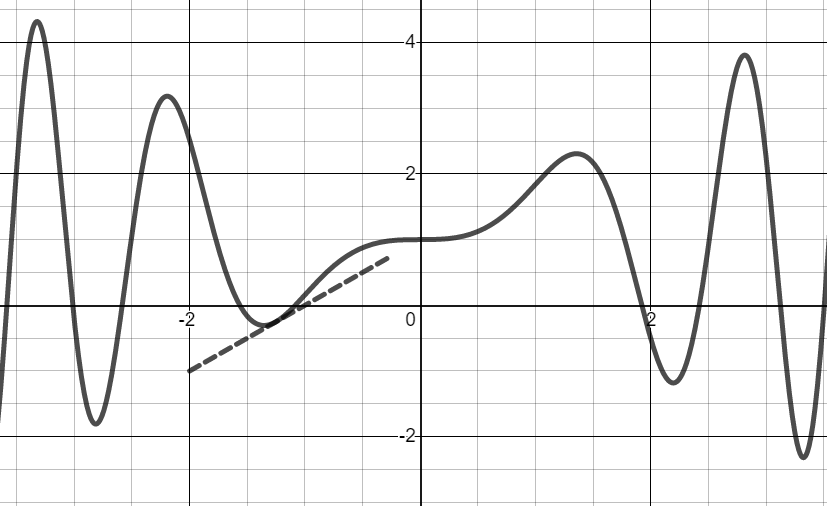
\includegraphics[width=14cm]{smooth}
		\caption{The function is smooth everywhere, there are no gaps or sharp transitions, and therefore it has a well defined tangent line at any point. One of these tangents is shown. The function that defines \textit{all} possible tangents is called the derivative.}\end{center}
\end{figure}
\section*{Rate of Change}
We will begin with the concept of average speed. If you travel a distance of 120 km in 2 hours then your average speed is 60 kph. 
\begin{center}
Average speed $ =\frac{\text{distance travelled}}{\text{time elapsed}}$
\end{center}\par
A distance/time graph can be drawn. The average speed can be expressed using function notation 
\begin{center}
Average speed $ =\frac{s (b) -s (a)}{b -a}$
\end{center}\par
Finding the average rate of change is important in many contexts and in fact the average rate of change can be defined for any function. 

The average rate of change of the function $y =f (x)$ is $\frac{\text{change in }y}{\text{change in }x}$ or $\frac{f (b) -f (a)}{b -a}$\hfill(1) 

The average rate of change is the slope of the \textbf{secant line} between $x =a$ and $x =b$ on the graph of $f$,\ that is the slope of the line that passes through $(a ,f (a))$ and $(b ,f (b))$. 

\example Calculate the average rate of change for the function $f (x) =x^{2} +4$ between the following points:
\begin{tasks}[counter-format=(tsk[1]),column-sep=3em](3)
\task $x =2$ and $x =6$ \\
\solution\\ Using the function notation in (1) above, \[\frac{f(2)-f(6)}{2-6}=\frac{8-40}{-4}\]
\[=\frac{-32}{-4}=8\]

\task $x =5$ and $x =10$ \\
\solution\\
\[\frac{f(5)-f(10)}{5-10}=\frac{29-104}{-5}=15\]

\task $x =a$ and $x =a +h$\\ ($h \neq 0$) \\
\solution\\
\[\frac{f(a)-f(a+h)}{a-(a+h)}\]
\[=\frac{a^2+4-([a+h]^2-4)}{a+h}\]
Can this be simplified further?
\end{tasks}
\begin{figure}\begin{center}
\includegraphics[width=12cm]{secant}
\caption{As the two points come closer together the secant line $ab$ gets shorter. When $b$ is at $a$ the secant line becomes a tangent line. See this \href{https://www.desmos.com/calculator/1zlwbppkuh}{animated with Desmos} (check the link on blackboard).}\end{center}
\end{figure}

%---------------------------------------------------
% 
%---------------------------------------------------
\subsection*{Tangents}
We now investigate the process of changing the value of $(b -a)$ in formula (1). As $(b -a)$ is made smaller and smaller the slope of the secant approaches the slope of the tangent at $x =a$. The notation for this process is as follows. 

\textbf{Definition:} The tangent line to the curve $y =f (x)$ at the point $P (a ,f (a))$ is the line through $P$ with slope $m =\Lim{x\to a}\frac{f (x) -f (a)}{x -a}$ provided that the \textit{limit} exists. This means that as the value of $x$ gets close to $a$ the function remains smooth. Imagine zooming in on a function, from far away it may appear smooth, but up close it could have some gaps or discontinuities.  Limits do not exist at sharp transitions in a graph, or where the function does not exist (think of piecewise functions). 

We sometimes refer to the slope of the tangent line to a curve at a point as the slope of the curve at that point. The idea is that if we zoom in far enough towards the point then the curve looks almost like a straight line. The more we zoom in the more the parabola looks like a straight line. 

\begin{figure}\begin{center}
		\includegraphics[width=12cm]{secant2tangent}
		\caption{A tangent can only touch the curve once. The slope of the tangent is perpendicular to the radius at the tangent point. This slope is called the rate of change or \textit{derivative} of the function at the point. See this \href{https://www.desmos.com/calculator/ialy1tknoo}{animated with Desmos} (check the link on blackboard).}\end{center}
\end{figure}

Using function notation for the tangent line is usually easier to use and is often preferred. The slope of the secant line between $x =a$ and $x =a +h$ is $\displaystyle \frac{f (a +h) -f (a)}{h}$. This looks familiar from \textsc{example} 3 above. We can now use this as a definition:

\begin{tcolorbox}
$$\text{slope }=m=\Lim{h\to 0} \frac{f(a+h)-f(a)}{h}$$
\end{tcolorbox}
This is limit notation, $\Lim{h\to 0} $, and we would say `the limit as $h$ approaches $0$'. Note that if $h=0$ the function is now undefined (math error). So $h$ is allowed to get close to zero, but not actually equal zero.



%---------------------------------------------------
% Derivatives from 1st Principles
%---------------------------------------------------
\section{Derivatives from 1st Principles}
Because the expression $\Lim{h \to 0}\frac{f (a +h) -f (a)}{h}$ occurs so widely it is given a special name and notation. 

The derivative of a function at a number $a$, denoted by $f^{ \prime } (a)$ is 
\begin{tcolorbox}
Definition of the derivative:\qquad$\displaystyle f^{ \prime } (a) =\Lim{h \to 0}\frac{f (a +h) -f (a)}{h}$
\end{tcolorbox}

The process of finding the derivative using the above definition is called finding the derivative \textit{from first principles}. So far we have found a derivative of a function $f$ at a fixed number $a$. If we replace $a$ in this equation with a variable $x$ we obtain 
\[f^{ \prime } (x) =\Lim{h \to 0}\frac{f (x +h) -f (x)}{h}\tag*{*Note the difference from above}\]
given any number $x$ for which this limit exists. We assign to $x$ the number $f^{ \prime } \left (x\right )$. So we can regard $f^{ \prime }$ as a new function which we call the derived function or the derivative of $x$. 

\subsection*{Derivatives of Polynomial Functions}
The constant function $f (x) =c$ is considered a polynomial of degree zero. Using the method of first principles we can find the derivative as follows: 
$$f^{ \prime } (x) =\Lim{h\to 0}\frac{f (x +h) -f (x)}{h} =\Lim{h\to 0}\frac{c -c}{h} =\Lim{h\to 0}0 =0$$

\subsection*{Higher Power Polynomials}
When $f (x) =x$ it can be shown from first principles that $f^{ \prime } (x) =1$. Similarly when $f (x) =x^{2\text{}}$it can be shown that $f^{ \prime } (x) =2 x$ and when $f (x) =x^{3}$ it can be shown that $f^{ \prime } (x) =3 x^{2}$. 

\example Find $f'(x)$ for $f (x) =x^{4}$ from first principles.

\solution \begin{align*}f^{ \prime } (x) &  = \Lim{h\to 0}\frac{f (x +h) -f (x)}{h} \\
 &  = \Lim{h\to 0}\frac{(x +h)^{4} -x^{4}}{h} \\
 &  = \Lim{h\to 0}\frac{x^{4} +4 x^{3} h +6 x^{2} h^{2} +4 x h^{3} +h^{4} -x^{4}}{h} \\
 &  = \Lim{h\to 0}\frac{4 x^{3} h +6 x^{2} h^{2} +4 x h^{3} +h^{4}}{h} \\
 &  = \Lim{h\to 0}(4 x^{3} +6 x^{2} h +4 x h^{2} +h^{3})\text{ here, substitute }h=0 \\
 f'(x)&  = 4 x^{3}\end{align*}

This pattern will follow for any similar polynomial: If $f (x) =x^{n}$ then $f^{ \prime } (x) =n x^{n -1}$. Or alternatively 
\begin{tcolorbox}
The Power Rule for Differentiation:\qquad$\displaystyle \frac{d}{d x} (x^{n}) =n x^{n -1}$
\end{tcolorbox}
	
This pattern implies that $n$ must be a positive integer. It can be shown that from the definition of a derivative $\frac{d}{d x} \genfrac{(}{)}{}{}{1}{x} = -\frac{1}{x^{2}}$ or $y =x^{ -1}$ then $\frac{d y}{d x} = -1 \times x^{ -2}$, which proves the power rule for $n = -1$. 

Similarly if the exponent is a fraction it can be shown that the power rule holds e.g. if $f (x) =\sqrt{x}$ then $f^{ \prime } (x) =\frac{1}{2 \sqrt{x}}$ or $f (x) =x^{\frac{1}{2}}$ then $f^{ \prime } (x) =\frac{1}{2} x^{ -\frac{1}{2}}$. It can be shown that the power rule holds for any real number $n$. 

%---------------------------------------------------
% Standard Derivatives
%---------------------------------------------------
\section{Standard Derivatives}
The basic functions have easily repeatable patterns to find their derivatives. The common ones are summarized in the table below:
\begin{center}
\begin{tabular}{ccll}	
	\toprule
	Function& Derivative&&Notes\\\midrule
	$f(x)$ & $f'(x)$  &&notation\\ \midrule
	$x^n$ & $nx^{n-1}$ &&`power rule'\\ \midrule
	$e^x$ & $e^x$  && exponential\\ \midrule
	$\ln(x)$ & $\frac{1}{x}$ &&logarithmic\\ \midrule
	$\sin(x)$ & $\cos(x)$  && \\ \cmidrule{1-2}
	$\cos(x)$ & $-\sin(x)$ && trigonometric\\ \cmidrule{1-2}
	$\tan(x)$ & $\sec^2(x)$ && \\ \bottomrule
\end{tabular}
\end{center}


\subsection*{The Natural Exponential}
Recall the natural exponential function from section~\ref{sec:naturalExponential}. Here we can see why precisely it is so special. Using limit notation, we can say that $e$ is the number such that $\Lim{h\to 0}\frac{e^{h} -1}{h} =1$. The derivative is:

\begin{tcolorbox}
The Derivative of the Natural Exponential Function
$$\frac{d}{d x} \left (e^{x}\right ) =e^{x}$$
\end{tcolorbox}

The natural exponential function is unique because \textbf{it has its own derivative!} Geometrically this means that the slope of the tangent at any point is the same as the y-coordinate, $f(x)$, of that point. 

%---------------------------------------------------
% max, min and tangents
%---------------------------------------------------
\section{Maximums, Minimums, and Tangents}
Turning points occur at the boundary between regions in a function.  A function that transitions from increasing to decreasing must have a turning point. In the function below, $f(-1)=2$ means the point $(-1,2)$ is a turning point. More specifically this is a local maximum of our function. It is the highest point in its \emph{local} neighbourhood. Notice that the other boundary has different properties: it is the lowest point. So $f(1)=-2$ means the point $(1,-2)$ is a local minimum.

The boundary means that the slope of the \textit{tangent} has gone from increasing to decreasing. Or from positive to negative. During this transition it had to go through zero, and so a turning point can be found anywhere the slope is equal to zero: $f'(x)=0$. Remember that the first derivative represents the slope of the function.
\clearpage
\begin{multicols}{2}
\example Find the turning points for \[f(x)=x^3-3x\]
\columnbreak
	\begin{center}
		\begin{tikzpicture}
		\begin{axis}[
		axis lines=center,
		ymax=4,ymin=-4,
		xmax=3,xmin=-3,
		xtick={-2,...,2},xticklabels={-2,-1,0,1,2},
		ytick={-2,...,2},yticklabels={-2,-1,0,1,2},
		xlabel=$x$,ylabel=$y$,
		]
		\addplot [<->,domain=-2.19:2.19,thick, samples=200, black] {x^3-3*x};
		\addplot [dashed,domain=0:2.5,thick, samples=200, black] {-2};
		\addplot [dashed,domain=-2.5:-0.5,thick, samples=200, black] {2};
		\addplot[mark=*] coordinates {(1,-2)};
		\addplot[mark=*] coordinates {(-1,2)};
		\node[anchor=south] at (axis cs:1,-3.1) {$f'(1)=0$};
		\node[anchor=south] at (axis cs:1.2,-3.6) {\footnotesize{local minimum}};
		\node[anchor=south] at (axis cs:-1.6,2.1) {$f'(-1)=0$};
		\node[anchor=south] at (axis cs:-1.6,3) {\footnotesize{local maximum}};
		\end{axis}
		\end{tikzpicture}
	\end{center}
\end{multicols}
\solution 
\begin{multicols}{2}
Set the derivative equal to zero and solve for values of $x$.
\begin{align*}
\frac{dy}{dx}&=3x^2-3\\
0&=3x^2-3\\
3&=3x^2\\
1&=x^2\\
x&=1, \,\mathrm{ and }\, x=-1
\end{align*}
Therefore the $x-$values of the turning points are 1 and $-1$. Note there are two turning points in our function so there should be two corresponding solutions.\\
\begin{align*}
f(1)&=(1)^3-3(1)\\
&=1-3=-2
\end{align*}
Therefore $(1,-2)$ is the first turning point. Similarly, $(-1,2)$ is found as the other turning point. These are both shown in the figure above.\end{multicols}

\subsection*{Second Derivative Test}\label{sec:2ndDerivativeTest}
We know from the graph that these turning points are maximum and minimum. The graph is not always provided to identify maxima and minima, so it helps to have a test to determine if a point is a max or min. 

We know first derivative represents the slope of the function. Looking at the parabola $y=x^2$ and following the function from left to right we can plot some values of the first derivative. The graph tells us that the turning point is at $(0,0)$ and is a minimum. The value of the 1st derivative is -2,-1,0,1,2 : these numbers are increasing. This trend is always true for a local minimum. 

How do we test for this trend of increasing slopes? The rate of change of the \emph{slopes} is the second derivative, and if this number (at the point $(0,0)$) is positive, then the point is a minimum.

This is called the second derivative test.\\
%maybe highlight box here%
\begin{tcolorbox}
	Second Derivative Test
	\begin{itemize}
		\item If $f'(x)=0$, and $f''(x)>0$, then the point $(x,f(x))$ is a local minimum. The graph in this neighbourhood is concave up.\\
		\item If $f'(x)=0$, and $f''(x)<0$, then the point $(x,f(x))$ is a local maximum. The graph in this neighbourhood is concave down.\\                          
	\end{itemize}
\end{tcolorbox}


%Example level: EASY
\example Use the second derivative test to determine if the turning point $(-1,2)$ is a maximum or minimum on the function $f(x)=x^3-3x$\\
\solution Find the second derivative and substitute the turning point.
\begin{align*}
f'(x)&=3x^2-3\\
f''(x)&=6x\\
f''(-1)&=6(-1)=-6\\
-6&<0
\end{align*}therefore the turning point $(-1,2)$ is a local maximum.

\subsection*{Points of Inflection}\label{sec:PointsOfInflection}
There is one last feature of the initial function that can be found. There is a point in between the maximum and minimum points where the change in slopes of the function change from decreasing to increasing. This is called a point of inflection. It is where the concavity of the function changes between down and up.
% include the plot file for
% point of inflection graph
\begin{center}
	\begin{tikzpicture}
	\begin{axis}[
	axis lines=center,
	ymax=4,ymin=-4,
	xmax=3,xmin=-3,
	xtick=\empty,ytick=\empty,
	xlabel=$x$,ylabel=$y$,
	]
	\addplot [<->,domain=-2.05:2.05,thick, samples=200, black] {x^3-3*x};
	\addplot[mark=*] coordinates {(0,0)};
	\addplot[mark=*] coordinates {(0,-3.5)};
	\addplot [dashed,<->,domain=-3:3,thick, samples=200, black] {-3.5};
	\node[anchor=south] at (axis cs:1.5,-3.5) {\footnotesize{concave up}};
	\node[anchor=south] at (axis cs:-1.5,-3.5) {\footnotesize{concave down}};
	\node[anchor=south] at (axis cs:1.5,2.5) {\footnotesize{point of inflection}};
	\draw[<-](axis cs:0.1,0.1)--(axis cs:1,2.5);
	\end{axis}
	\end{tikzpicture}
\end{center}
The second derivative test can be used to determine if a function is concave-up ($>0$) or concave down ($<0$). Note there is no $=$ in these inequalities. In between is where the point of inflection can be found:
\begin{tcolorbox}
	Second Derivative Test for Concavity
	\begin{itemize}
		\item If $f''(x)=0$, then the point $(x,f(x))$ is a point of inflection.\\                         
	\end{itemize}
\end{tcolorbox}

%Example level: EASY
\example Find where the function changes from concave-up to concave-down.\\
\[f(x)=3x^3-12x^2+7\]
\solution Find the second derivative and set equal to zero to find the point of inflection.
\begin{multicols}{2}
\begin{align*}
f'(x)&=9x^2-24x\\
f''(x)&=18x-24\\
0&=18x-24\\
\frac{4}{3}&=x
\end{align*}
Sub back into $f(x)$ to find the $y-$value:\\
\begin{align*}
f\left(\frac{4}{3}\right)&=3\left(\frac{4}{3}\right)^3-12\left(\frac{4}{3}\right)^2+7\\
&=-7\tfrac{2}{9}
\end{align*}
Therefore, the point $\left(\tfrac{4}{3},-7\frac{2}{9}\right)$ is a point of inflection.
\end{multicols}

%---------------------------------------------------
% The Product, quotient and chain rules
%---------------------------------------------------
\section{The Product, Quotient, and Chain Rules}

%-----------------------------------------------
\subsection*{The Product Rule}
Let $f (x) =x$ and $g (x) =x^{2}$. What is the derivative of $f (x) \times g (x)$? The question helps to show that the answer is NOT $f^{ \prime } (x) \times g^{ \prime } (x)$ 

$f (x) \times g (x) =x \times x^{2} =x^{3}$ and we know the derivative of $x^{3}$ is $3 x^{2}$. Also we know that $f^{ \prime } (x) =1$ and $g^{ \prime } (x) =2 x$ so $f^{ \prime } (x) \times g^{ \prime } (x) =1 \times 2 x =2 x$ not $3 x^{2}$. 

So the derivative of the product of two functions is not the product of the derivatives of each function. In symbols this can be written 
\[\left (f g\right )^{ \prime } \neq f^{ \prime } g^{ \prime }\]
\textbf{Theorem} If $f$ and $g$ are both differentiable then 
\begin{tcolorbox}
	\[\frac{d}{d x} \left [f (x) g (x)\right ] =f (x) \frac{d}{d x} \left [g (x)\right ] +g (x) \frac{d}{d x} \left [f (x)\right ]\]
	\end{tcolorbox}
The Product rule is often seen in an abbreviated form as $\displaystyle \left(u v\right)^{\prime} =uv^{\prime} +vu^{\prime}$.

\example Find the derivative of $f(x)=x^2e^x$.\medskip\\
\solution Use the product rule:
$$f'(x)=(2x)(e^x)+(x^2)(e^x)$$
This could be simplified by factoring: $f'(x)=e^x(2x+x^2)$ but is not mandatory.
\hrule
\example Differentiate $f=4\pi x\sin x$.\medskip\\
\solution Use the product rule. $4\pi$ is a constant.
$$f'=(4\pi)(\sin x)+(4\pi x)(\cos x)$$.
\hrule
\example If $g(x)=\frac{e^x}{3}\sqrt{x+2}$, find $g'(x)$.\medskip\\
\solution Convert the root to power form and use the product rule.
\begin{align*}
g(x)&=\frac{1}{3}e^x(x+2)^{\frac{1}{2}}\\
g'(x)&=\left[\frac{1}{3}e^x\right]\left[(x+2)^{\frac{1}{2}}\right]+\left[\frac{1}{3}e^x\right]\left[\frac{1}{2}(x+2)^{-\frac{1}{2}}\right]\\
&=\frac{e^x}{3}\sqrt{x+2}+\frac{e^x}{6\sqrt{x+2}}
\end{align*}

%-----------------------------------------------
\subsection*{The Quotient Rule}
Let $u =f (x)$ and $v =g (x)$ be differentiable functions of $x$ then we can show that
\begin{tcolorbox}
	\[\frac{d}{d x} \genfrac{[}{]}{}{}{f (x)}{g (x)} =\frac{g (x) \frac{d}{d x} \left [f (x)\right ] -f (x) \frac{d}{d x} \left [g (x)\right ]}{\left [g (x)\right ]^{2}}
\]
\end{tcolorbox}
or in abbreviated form as
\begin{equation*}\genfrac{(}{)}{}{}{u}{v}^{ \prime } =\frac{v u^{ \prime } -u v^{ \prime }}{v^{2}}
\end{equation*}
\hrule
\example Differentiate with the quotient rule: $y=\frac{(s-1)(s+3)}{e^{2s}}$\medskip\\
\solution Expand the numerator first and then differentiate\\
\begin{align*}y&=\frac{s^2+2s-3}{e^{2s}}\\
y'&=\frac{(2s+2)(e^{2s})-(s^2+2s-3)(e^{2s})\cdot2}{(e^{2s})^2}\\
y'&=\frac{-2(s^2+s-4)}{e^{2s}}
\end{align*}
\hrule
\example Find $f'$, given $f=\frac{\sin x}{x}$\medskip\\
\solution $$f'=\frac{\cos(x)\cdot x-\sin(x))}{x^2}=\frac{x\cos(x)-\sin(x))}{x^2}$$
\hrule
\example Find $f'$, given $\displaystyle f=\frac{\ln x}{e^x}$\medskip\\
\solution $$f'=\frac{(\frac{1}{x})(e^x)-(\ln x)(e^x)}{e^{x^2}}$$
$$=\frac{1-x\ln x}{xe^x}$$




%-----------------------------------------------
\subsection*{Chain Rule}
When functions are combined with other functions, they are often called composite functions. These require special treatment when differentiating.

Let $f (x) =x^{2}$ and $g (x) =2 x +1$ then $\left (f \circ g\right )$ This means $f$ `composed of' $g$ is $f \left (g \left (x\right )\right ) =f (2 x +1) =\left (2 x +1\right )^{2}$. 

Also, $g$ `composed of' $f$ would be: $\left (g \circ f\right ) (x) =g \left (x^{2}\right ) =2 \left (x^{2}\right ) +1 =2 x^{2} +1$. 

The differentiation rules we have met so far allow us to differentiate pairs of functions that have been added, subtracted, multiplied or divided. They do not allow us to differentiate an expression that is made from a function that is within another function.

The following are all examples of composite functions. 
\begin{enumerate}
\item We can differentiate $x^{2}$ but we can't use the same procedure to differentiate $\left (1 -x\right )^{2}$. Here we can imagine if  $f (x) =x^{2}$ and $g (x) =1 -x$ then $\left (f \circ g\right ) (x) =f (1 -x) =\left (1 -x\right )^{2}$.

\item We can differentiate $\frac{1}{x^{2}}$ but we can't use the same procedure to differentiate $\frac{1}{x^{2} +1}$. 

\item We can differentiate e$^{x}$ but we can't use the same procedure to differentiate $e^{x^{2}}$. 
\end{enumerate}

A name often used for functions of this type is \emph{function of a function.} 

Once we recognise we are dealing with a composite function we need a procedure to differentiate it. You will find that you are far more likely to be required to differentiate a composite function in a practical situation than a simple one. It can be proved that the derivative of the composite function $f \circ g$ is the product of the derivatives of $f$ and $g$. This important rule is given the name the \emph{Chain Rule}. A substitution method is often used to add clarity to the differentiation process. 

Let
$y =u^{2}$ and let $u =1 -x$. Then $\frac{d y}{d u} =2 u$ and $\frac{d u}{d x} = -1$. Now $\frac{d y}{d x} =\frac{d y}{d u} \cdot \frac{d u}{d x} =2 u \times ( -1) = -2 u = -2 (1 -x) =2 (x -1)$. 

The Leibniz form of the Chain Rule $\displaystyle \frac{d y}{d x} =\frac{d y}{\cancel{d u}} \frac{\cancel{d u}}{d x}$ is what gives the rule its name. Because of the apparent cancelling it is particularly
easy to learn in this form. 

As an aside let us verify the rule for this example. Given
$y =(1 -x)^{2}$. We will expand the right hand side of the equation. It
becomes $y =x^{2} -2 x +1$. So $y^{ \prime } =2 x -2 =2 (x -1)$ as before. 

Using function notation the Chain Rule states: If $f$ and $g$ are both differentiable and $F =f \circ g$ is the\ composite function $F (x) =f (g (x))$, then $F$ is differentiable and $F^{ \prime } =f^{ \prime } (g (x)) g^{ \prime } (x)$. 

\subsection*{A Comment on the Leibniz form of the Chain Rule}
$\frac{d y}{d x} =\frac{d y}{d u} \cdot \frac{d u}{d x}$ gives the impression that the $d u$ could cancel but remember we have not defined $d u$. We have defined $\frac{d y}{d u}$ as the rate of change of $y$ with respect to $u$ and $\frac{d u}{d x}$ as the rate of change of $u$ with respect to $x$. However the apparent cancelling helps us to remember the way the differentials
are arranged. it also helps us to accept the extension of the Chain Rule to cover a function of a function of
a function etc. e.g.
\begin{align*}\text{Let}y &  = f (u)\text{,}u =g (v)\text{and}v =h (x) \\
\text{Then}\frac{d y}{d x} &  = \frac{d y}{d u} \cdot \frac{d u}{d v} \cdot \frac{d v}{d x}\end{align*}

\example Find $F^{ \prime } (x)$ when $F (x) =\frac{1}{x^{2} +1}$. \\
\solution Using function notation $F (x) =\left (f \circ g\right ) (x) =f (g (x))$ \\
where $$f (u) =u^{ -1} \text{ and }g (x) =x^{2} +1$$
\begin{equation*}f^{ \prime } (u) = -u^{ -2}\text{and}g^{ \prime } (x) =2 x
\end{equation*}
and 
\begin{align*}F^{ \prime } (x) &  = f^{ \prime } (g (x)) g^{ \prime } (x) \\
 &  = \frac{ -1}{(x^{2} +1)^{2}} \cdot 2 x \\
 &  = \frac{ -2 x}{\left (x^{2} +1\right )^{2}}\end{align*}
Using the Leibniz notation let $u =x^{2} +1$ and $y =u^{ -1}$ then
\begin{align*}F^{ \prime } (x) &  = \frac{d y}{d u} \frac{d u}{d x} = -u^{ -2} \left (2 x\right ) \\
 &  = \frac{ -1}{\left (x^{2} +1\right )^{2}} \left (2 x\right ) =\frac{ -2 x}{\left (x^{2} +1\right )^{2}}\end{align*}

To use the method we need to bring a new variable into the problem we are trying to solve. It
is recommended that you use the variable $u$ wherever possible so that you follow through using a pattern you are familiar with. 

In summary: if $g$ is differentiable at $x$ and $f$ is differentiable at $g (x)$, then the composite function $F =f \circ g$ defined by $F (x) =f (g (x))$ is differentiable at $x$ and $F^{ \prime }$ is given by the product
\begin{tcolorbox}
\[F^{ \prime } (x) =f^{ \prime } (g (x)) \cdot g^{ \prime } (x)\]
\end{tcolorbox}
In Leibniz notation, if $y =f (u)$ and $u =g (x)$ are both differentiable functions, then
\begin{tcolorbox}
\[\frac{d y}{d x} =\frac{d y}{d u} \cdot \frac{d u}{d x}\]
\end{tcolorbox}

The Chain Rule will be found in many situations where functions are added, subtracted, multiplied or divided. As an example we will focus on combining the Chain Rule with the Product Rule, however any combination of these rules could be found in a problem. 

\example Differentiate $x e^{ -x^{2}}$. 

\solution We can see that there is a product of two functions present in this example, i.e. $f (x) =x$ and $g (x) =e^{ -x^{2}}$. Also $g (x)$ is a composite function. 

We have from the Product Rule
\begin{equation*}\left (f g\right )^{ \prime } =f g^{ \prime } +g f^{ \prime }
\end{equation*}

By inspection we can see that of the four expressions on the right side of this equation $f$, $g$ and $f^{ \prime }$ can be put into the equation immediately and only $g^{ \prime }$ requires some effort to be worked out. 

$g (x)$ is a composite function so $g^{ \prime } (x)$ is computed using the Chain Rule. 

Let $u = -x^{2}$ then $\frac{d u}{d x} = -2 x$. Also $g (u) =e^{u}$ so $\frac{d g}{d u} =e^{u}$.
\begin{align*}\frac{d g}{d x} &  = \frac{d g}{\cancel{d u}}\cdot \frac{\cancel{d u}}{d x} \\
 &  = e^{u} \cdot  -2 x \\
 &  = e^{ -x^{2}} \cdot  -2 x \\
 &  =  -2 x\; e^{ -x^{2}} \\
\text{So }g^{ \prime } (x) &  =  -2 x\; e^{ -x^{2}}\end{align*}

Putting this all together
\begin{align*}\left (f g\right )^{ \prime } &  = f g^{ \prime } +g f^{ \prime } \\
 &  = x \cdot  -2 x\; e^{ -x^{2}} +e^{ -x^{2}} \cdot 1 \\
 &  = e^{ -x^{2}} \left [1 -2 x^{2}\right ]\end{align*}

%---------------------------------------------------
% Parametric Differentiation
%---------------------------------------------------
\section{Parametric Differentiation}
Parametric Curves $x$ and $y$ are both given as functions of a third variable $t$ (called the \emph{parameter}). Let the equations be
\begin{equation*}x =f (t)\text{ and }y =g (t)
\end{equation*}

Each value of $t$ gives a point $(x ,y)$. As $t$ varies the point $(x ,y) =(f (t) ,g (t))$ traces out a curve in the coordinate plane called a \emph{parametric curve}. This is useful for functions that violate the vertical line test (see Section~\ref{sec:functions}) such as a circle, $x^2+y^2=r^2$, because only proper functions can be differentiated.

Both the fish and atomic-looking-thingy below can be plotted using parametric equations.
\begin{figure}[H]
	\begin{subfigure}[b]{0.5\textwidth}
		\centering
		\resizebox{\linewidth}{!}{
			\begin{tikzpicture}
			\begin{axis}[
			scale=1.2,
			axis lines=center,%width=4cm,height=4cm,
			ymax=2,ymin=-2,
			xmax=2,xmin=-2,
			xtick={-2,-1.5,-1,1,2},
			xlabel=$x$,ylabel=$y$,%	ytick=\empty,	
			]
			\addplot[domain=0:4*360, samples=200, thick] ({1.5*cos(x)},{-0.667*cos(1.5*x)});
			\addplot[mark=*] coordinates {(-1.5,0)};	
			\addplot[mark=*] coordinates {(1.5,-0.667)};
			\draw[->,ultra thick](axis cs:1.4,0.57) -- (axis cs:1.5,0.667);
			\node[anchor=south] at (axis cs:1.5,-1.1) {$t=0$};
			\node[anchor=south] at (axis cs:-1.5,-0.8) {$t=\pi$};		
			\end{axis}
			\end{tikzpicture}	
		}  \caption{fish: $\displaystyle x=\frac{3\cdot\cos t}{2},\, y=-\frac{2}{3}\cos\left(\frac{3t}{2}\right)$}
	\end{subfigure}
	\begin{subfigure}[b]{0.5\textwidth}
		\centering
		\resizebox{\linewidth}{!}{
			\begin{tikzpicture}
				\begin{axis}[
				scale=1.2,
				axis lines=center,%width=4cm,height=4cm,
				ymax=2,ymin=-2,
				xmax=2,xmin=-2,
				xtick={-2,-1,1,2},
				xlabel=$x$,ylabel=$y$,%	ytick=\empty,	
				]
				\addplot[domain=0:4*360, samples=200, thick] ({-1.5*sin(x)},{cos(1.5*x)});	
				\end{axis}
		\end{tikzpicture}	
		}  \caption{superhero logo: $\displaystyle x=-\frac{3}{2}\sin(t),\,y=\sin\left(\frac{3t}{2}\right)$}
	\end{subfigure}
\end{figure}
To find the point at the mouth of the fish in terms of $t$, we must solve the equations for $x=-1.5$, or $y=0$. As $t$ increases, the plot is drawn. 
\begin{equation*}
	\begin{aligned}[c]
x&=\frac{3\cdot\cos t}{2}\\
-1.5&=\frac{3\cdot\cos t}{2}\\
-1&=\cos t \\
t&=\pi\\
	\end{aligned}\qquad\qquad
	\begin{aligned}[c]
	 \text{check that }y&=0\\
	 y&=-\frac{2}{2}\cos\left(\frac{3\pi}{2}\right)\\
	y&=-\frac{2}{3}\cdot 0\\
	y&=0\\
	\end{aligned}
\end{equation*}
The point $t=0$ corresponds to $x=1.5$, and $y=-\frac{2}{3}=$ which is shown as a point on the tail.
\exercise In which direction is the superhero logo drawn? Where does it start?\\
\subsection*{Using the Chain Rule to find the Derivative $\frac{d y}{d x}$}
Given\ the parametric equations $x =f (t)$ and $y =g (t)$ define a parametric curve. If $f$ and $g$ are both differentiable the Chain Rule gives
\begin{equation*}\frac{d y}{d t} =\frac{d y}{\cancel{d x}} \cdot \frac{\cancel{d x}}{d t}
\end{equation*}

provided $y$ is also a differentiable function of $x$. So provided $\frac{d x}{d t} \neq 0$
\[\frac{d y}{d x} = \frac{d y}{d t} \div \frac{d x}{d t}\]
When dividing fractions remember to `invert and multiply'\\
\[\frac{d y}{d t} \times \frac{d t}{d x}=\frac{dy}{dx}\]

\example Find the derivative, $\frac{dy}{dx}$, of the fish in part (a).\medskip\\
\solution Differentiate each equation and combine with the chain rule to find $\frac{dy}{dx}$.\\
\begin{align*}x&=\frac{3\cos t}{2} &y=-\frac{2}{3}\cos\left({\frac{3t}{2}}\right)\\
\frac{dx}{dt}&=-\frac{3}{2}\sin t &\frac{dy}{dt}=-\frac{2}{3}\cdot-\sin \left({\frac{3t}{2}}\right)\cdot\frac{3}{2}\\
&&\frac{dy}{dt}=\sin \left({\frac{3t}{2}}\right)\\
\end{align*}
Now, using the chain rule, note $\frac{dx}{dt}$ must be inverted:\\
\begin{align*}\frac{dy}{dx}&=\frac{dy}{dt}\cdot\frac{dt}{dx}\\
&=\sin \left({\frac{3t}{2}}\right)\cdot \frac{1}{-\frac{3}{2}\sin t }\\
&=\frac{-2\sin \frac{3t}{2}}{3\sin t}
\end{align*}
Compare your derivatives, $y'$ and $x'$, with the superhero logo plot from part (b).
%---------------------------------------------------
% Related Rates
%---------------------------------------------------
\section{Related Rates}
The concept of related rates is best understood by exploring some examples. 

\examq Air is being pumped into a spherical balloon so that its volume is increasing at a rate of 50 $cm^{3}$/$\mbox{s}$. How fast is the radius of the balloon increasing when the diameter is 50 $\mbox{cm}$? \\
\solution The volume of a sphere is $\frac{4}{3}\pi r^3$. Find the derivative with respect to radius.
\[\frac{d V}{d r} =4 \pi r^2\]
We are looking for ``how fast'' (time) and radius ($r$), or $\frac{dr}{dt}$. From the Chain Rule we can write
\[\frac{d V}{d t} =\frac{d V}{d r} \cdot \frac{d r}{d t}\]
Substituting $\frac{d V}{d t} =50$ and $\frac{d V}{d r} =4 \pi  r^{2}$ we get
\begin{align*}50 &  = 4 \pi  r^{2} \cdot \frac{d r}{d t} \\
\frac{d r}{d t} &  = \frac{50}{4 \pi  r^{2}} \\
\end{align*}
Now we substitute $r =25$. (Diameter $ =50$ so radius $ =25$)
\begin{align*}\frac{d r}{d t}_{r =25} &  = \frac{50}{4\pi(25)^2} \\
&  = \frac{1}{50 \pi }\approx 0.00637\end{align*}
Therefore the radius is increasing at the rate of $\displaystyle\frac{1}{50 \pi } \mbox{cm}$/$\mbox{s}$ 

\example A ladder $5$ $\mbox{m}$ long rests against a vertical wall. If the bottom of the ladder slides away from the wall at the rate of $0.5$ $\mbox{m}$/$\mbox{s}$ how fast is the top of the ladder sliding down the wall when the bottom of the ladder is $3$ $\mbox{m}$ from the wall? 

\solution Let the origin be placed at the corner where the wall meets the floor, let $x$ be the distance of the foot of the ladder from the wall and let $y$ be the distance of the top of the ladder from the corner. The ladder forms a right angled triangle whose sides are $x$, $y$ and with hypotenuse $5$. We are given that $\frac{d x}{d t} =0.5$ and are asked to find $\frac{d y}{d t}$ when $x =3$. 

Pythagoras' theorem gives
\begin{equation}x^{2} +y^{2} =5^{2}\tag{1}
\end{equation}

Differentiate equation (1) with respect to $t$. Note that this derivative uses a technique called implicit differentiation. 
\begin{equation*}2 x \frac{d x}{d t} +2 y \frac{d y}{d t} =0
\end{equation*}

Solve for $\frac{d y}{d t}$
\begin{equation*}\frac{d y}{d t} = -\frac{x}{y} \cdot \frac{d x}{d t}
\end{equation*}

Using the Pythagorean theorem with $x=3$ and the hypotenuse $=5$, $y=4$ 

Substitute $\frac{d x}{d t} =0.5$, $x =3$ and $y =4$
\begin{align*}\frac{d y}{d t} &  =  -\frac{3}{4} \cdot 0.5 \\
 &  =  -0.375\end{align*}

The top of the ladder is moving vertically downwards at the rate of 0.375 $\mbox{m}$/$\mbox{s}$ 

\example A water tank has the shape of an inverted circular cone with a base radius of $2$ $\mbox{m}$ and height of $4$ $\mbox{m}$. If water is being pumped into
the tank at a rate of $2$ $\mathrm{m}^{3}$/$\mbox{min}$ find the rate at which the water level is rising when the water is $3$ $\mbox{m}$ deep. 

\solution Let $V$, $r$ and $h$ be the volume of water the radius of the surface and the height at time $t$. We are given
\begin{equation*}\frac{d V}{d t} =2\text{}\mathrm{m}^{3}/\mbox{min}
\end{equation*}

We are asked to find $\frac{d h}{d t}$ when $h =3$. 

Draw a diagram to show that the relationship between $r$ and $h$ can be found by similar triangles.
\begin{align}\frac{r}{h} &  = \frac{2}{4} \nonumber  \\
r &  = \frac{h}{2} \tag{1}\end{align}

The formula for the volume is
\begin{equation}V =\frac{1}{3} \pi  r^{2} h\tag{2}
\end{equation}

Substituting equation (1) in equation (2)
\begin{align*}V &  = \frac{1}{3} \pi  \genfrac{(}{)}{}{}{h}{2}^{2} h \\
 &  = \frac{\pi }{12} h^{3}\end{align*}

Differentiate with respect to $t$
\begin{align*}\frac{d V}{d t} &  = \frac{\pi }{12} \cdot 3 h^{2} \cdot \frac{d h}{d t} \\
 &  = \frac{\pi }{4} h^{2} \cdot \frac{d h}{d t}\end{align*}

So
\begin{equation*}\frac{d h}{d t} =\frac{4}{\pi  h^{2}} \cdot \frac{d V}{d t}
\end{equation*}

Substitute $h =3$ and $\frac{d V}{d t} =2$
\begin{align*}\frac{d h}{d t} &  = \frac{4}{\pi  \left (3\right )^{3}} \cdot 2 \\
 &  = \frac{8}{9 \pi }\end{align*}

The water level is rising at the rate of $\frac{8}{9 \pi }$ $\mbox{m}$/$\mbox{min}$. 

%---------------------------------------------------
% Optimisation
%---------------------------------------------------
\section{Optimisation}\label{sec:Optimisation}
Optimisation is the process of using calculus to find the best result for a situation involving a changing quantity (variable). Examples include  maximizing profit, minimizing cost, maximizing volume, minimizing amount materials used, and so on. As long as the quantities in question can be represented by a function, calculus can used to find the special points of the function and their nature.

\begin{tcolorbox}
	A general method to approach an optimisation problem             
	\begin{enumerate}
		\item Write down the known variables and draw a diagram
		\item Form an equation of the situation by placing the unknown variable in terms of the known variables
		\item Use the facts of the problem to reduce the expression until it becomes a relationship between the unknown quantity and one of the known quantities
		\item Optimize by finding a maximum or minimum value
	\end{enumerate}
\end{tcolorbox}

%Example level: EASY
\example A farmer wishes to fence a paddock using an existing wall as one side of the paddock. She has 100 meters of fencing and wants to know the dimensions of the paddock to enclose the maximum area.
% include the plot file for
% optimisation paddock
\begin{center}
	\begin{tikzpicture}
	\usetikzlibrary{patterns}
	\draw [thick](0,0) -- (0,3) -- (5,3) -- (5,0);
	\draw [dashed](-2,0) -- (7,0);
	\draw[pattern=north west lines, pattern color=gray!50, draw=none] (0,0) rectangle (5,3);
	\node at (2.5,-0.5) {existing wall};
	\draw [<->,thick] (5.3,0)--(5.3,3);
	\node at (7,1.5){fence length 1};
	\draw [<->,thick] (0,3.3)--(5,3.3);
	\node at (2.5,3.7){fence length 2};
	\node [text width=2cm, fill=white]at (2.5,1.5){area of the paddock};
	\end{tikzpicture}	
\end{center}
\solution Following the steps outlined above, draw a diagram and label the variables. Let $T$ represent the total fence length which cannot be more than 100m. Write this as an equation: $T=100$. There are 3 individual lengths that make up the total, so let $l$ represent the long side of the paddock, and $w$ represent the short side. 
\begin{align*}
T&=l+2w\\
100&=l+2w
\end{align*}
The quantity to be optimised is area ($A$) of the paddock (remember it is a rectangle):
\begin{align*}
A=lw
\end{align*}
The next step is to represent the quantity to be optimised (area) as a function of one other variable. We can rearrange our earlier equation to solve for length: $l=100-2w$. This can now be substituted into the area equation:
\begin{align*}
A&=lw\\
&=\left(100-2w\right)w\\
&=100w-2w^2
\end{align*}
This is now an equation that can optimised using calculus.
\begin{align*}
\frac{dA}{dw}&=100-4w\\
0&=100-4w\\
w&=25
\end{align*}
Therefore the paddock width is 25 meters to maximize the total area. Going back to the original constraint of 100m total length means that the paddock length is $100-2(25)=50$ meters.\\
\rule{6.8cm}{0.5pt}\\
%Example level: EASY
\example A cylindrical can is to be made to hold 1 litre of oil. Find the dimensions that will minimise the cost of the aluminium to manufacture the can. Note that 1 L = 1000 cm$^3$.\\

\begin{figure}[h]
	\centering
	\begin{subfigure}[h]{0.4\textwidth}
		\includegraphics[width=\textwidth]{graphics/oilCan}
	\end{subfigure}
	\begin{subfigure}[h]{0.4\textwidth}
		\begin{tikzpicture}
		\draw [thick](0,-1)rectangle(3,4);
		\draw [<->,thick] (0,-1.3)--(3,-1.3) node[below,xshift=-1.5cm]{height of can};
		\draw [<->,thick] (0.5,-1)--(0.5,4) node[below,yshift=-2.5cm,rotate=90]{circumference};
		\draw [thick](-1.5,1.5) circle [radius=1.5];
		\draw [thick](4.5,1.5) circle [radius=1.5];
		\draw[->,thick](-1.5,1.5)--(-0.25,2.3);
		\node at (-.9,1.5){$r$};
		\filldraw (-1.5,1.5) circle (2pt) ;
		\end{tikzpicture}	
	\end{subfigure}
\end{figure}	

\solution The minimum cost of the aluminium will be the minimum surface area of the cylinder. The can can be deconstructed into two circles and a rectangle. We will label the variables required to calculate area.

Let $SA$ represent surface area of the can. The total surface area is:
\begin{align*}
SA&=\pi r^2 + \pi r^2 + \left(\textrm{height}*\textrm{circumference}\right)\\
&=2\pi r^2+2\pi rh
\end{align*}
Note that we have 2 variables that are unknown, $r$, and $h$. We need to express one variable in terms of the other in order to proceed. Use the additional information in the problem. The volume of the can must be 1000 cm$^3$.
\begin{align*}
V&=\pi r^2 h\\
1000&=\pi r^2 h\\
h&=\frac{1000}{\pi r^2}
\end{align*}
Substitute this form for $h$ into the surface area function:
\begin{align*}
\text{SA}&=2\pi r^2+2\pi rh\\
&=2\pi r^2+2\pi r\left(\frac{1000}{\pi r^2} \right)\\
&=2\pi r^2+\frac{2000}{r}
\end{align*}
This function is now the surface area in terms of a single variable, $r$, and can be optimised:
\begin{align*}
\frac{d(\text{SA})}{dr}&=4\pi r-\frac{2000}{r^2}\\
0&=4\pi r-\frac{2000}{r^2}\\
&=4\pi r^3-2000\\
r^3&=\frac{2000}{4\pi}\\
r&=5.419 \,\textrm{cm}
\end{align*}
Therefore the final dimensions of the can optimised for minimum cost are radius$=5.42$ cm, and height$=10.8$ cm. 



%---------------------------------------------------
% Chapter Exercises in a separate file
%---------------------------------------------------
% \clearpage
 \section{Chapter Exercises}
 \subimport{}{differentiationExercises}

%---------------------------------------------------
% Integration
%---------------------------------------------------
\chapter[Integration]{Integration $<\int>$}
In mathematics we are often given a function $f$ and asked to find a function $F$ whose derivative is $f$. $\;F$ in this situation is called the integral of $f$. It is usual to develop a list of integrals by differentiating a range of functions then using those to work backwards. The terms integration and anti-differentiation are synonymous. Generally we will use the term integration, however, both are acceptable.

The process of `reversing' or `undoing' a derivative has its own symbol, the integrand: $\displaystyle\int$
\begin{tcolorbox}
	\[\int f'(x) dx = f(x)+C\]
\end{tcolorbox}

%---------------------------------------------------
% Standard Integrals
%---------------------------------------------------
\section{Standard Integrals}
It is not the intention here to list all of the rules that are required however at this stage let us explore the Power Rule to establish a rule for integrating an expression of the form $y =x^{n}$ \\

\begin{center}
\begin{tabular}[c]{p{1.5cm}p{1.5cm}}\toprule
function $f(x)$  & derivative $f'(x)$  \\
\midrule
$x$  & $1$  \\
$x^{2}$  & $2 x$  \\
$x^{3}$  & $3 x^{2}$  \\
$x^{4}$  & $4 x^{3}$  \\
\bottomrule
\end{tabular}\ or
\
\begin{tabular}[c]{ll}\toprule
 $f$  & $f'$  \\
\midrule
$x$  & $1$  \\
$\frac{1}{2} x^{2}$  & $x$  \\
$\frac{1}{3} x^{3}$  & $x^{2}$  \\
$\frac{1}{4} x^{4}$  & $x^{3}$  \\
\bottomrule
\end{tabular}\ now, in reverse \
\begin{tabular}[c]{p{2cm}p{2.5cm}}\toprule
derivative $f'(x)$  &  integral $\int f'(x)=f(x)$  \\\midrule
$1$  & $x +C$  \\
$x$  & $\frac{1}{2} x^{2} +C$  \\
$x^{2}$  & $\frac{1}{3} x^{3} +C$  \\
$x^{3}$  & $\frac{1}{4} x^{4} +C$  \\
\bottomrule
\end{tabular}
\end{center}
\bigskip This establishes the pattern and if you think about the rule for differentiating $y =x^{n}$ you can soon establish the rule for integrating $x^{n}$.
\begin{tcolorbox}
	The \textbf{Power Rule} for integrating polynomials
\[\int x^n dx = \frac{x^{n +1}}{n +1} +c, \text{ where }n \neq  -1
\]
\end{tcolorbox}

\begin{equation*}\text{ If }f (x) =x^{ -1}\text{ then the integral of }f\text{ is }\ln  \left \vert x\right \vert  +c\text{ or }\ln  \left \vert k x\right \vert
\end{equation*}
All of the differentiation rules we have met so far lead to integration rules. For instance we can establish standards for $\sin  x$, $\cos  x$, and $\sec ^{2} x\text{.}$ The standard integrals are summarized in the table below.
\renewcommand\arraystretch{1.5}
\begin{center}
	\begin{tabular}{cc}
		\toprule
		function&integral\\
		$f(x)$  &  $\int f(x)dx$ \\ \midrule
		$x^n, n \neq -1$ & $\frac{x^{n+1}}{n+1}+C$\\ 
		$e^x$ & $e^x+C$\\ 
		$\frac{1}{x}$ & $\ln|x|+C$\\ 
		$\sin(x)$ & $-\cos(x)+C$ \\ 
		$\cos(x)$ & $\sin(x)+C$ \\ 
		$\sec^2(x)$ & $\tan(x)+C$ \\ \bottomrule
	\end{tabular}
\end{center}

To allow us to combine these integrals and thus extend the range of questions we can tackle we use two important rules for integrals 
\begin{tcolorbox}
\textbf{Sum Rule} The integral of the sum of two functions is the sum of the integrals of the functions.
\[\int \left [f (x) +g (x)\right ]\; d x =\int f (x)\; d x +\int g (x)\; d x\]
\end{tcolorbox}
This is easily extended to the sum or difference of a number of functions. 
\begin{tcolorbox}
\textbf{Constant Multiple Rule} The integral of a constant times a function is the constant times the integral of the function.
\[\int c f (x)\; d x =c \int f (x)\; d x
\]\end{tcolorbox}

\example Integrate the following functions; find $\displaystyle\int f(x)$.
\begin{tasks}(2)
	\task $f(x) =3x^{2}$ \medskip\\
	\solution Applying the power rule:\\
\begin{align*}\int 3x^{2}\,dx&=\frac{3x^{2+1}}{2+1}+C\\
	&=x^3+C\end{align*}
\task $f (x) =7$ \medskip \\
\solution Here we are integrating a constant:\\
\[\int 7\,dx=7x+C\]

\task $f(x) =x^{\frac{2}{3}}$ \medskip\\
\solution The power rule still applies to fractional indices:\\
\begin{align*}\int x^{\frac{2}{3}}\,dx&=\frac{x^{\frac{2}{3}+1}}{\frac{2}{3}+1}+C\\
&=\frac{3 x^{5/3}}{5}+C \end{align*}

\task $f (x) =\frac{1}{2 \sqrt{x}} +\frac{1}{\sqrt{2}}$ \medskip\\
\solution Here we need to combine the sum rule and the power rule:\\
\begin{align*}
\int f(x)\,dx &= \int(\frac{1}{2 \sqrt{x}}) \,dx+\int(\frac{1}{\sqrt{2}}) \,dx\\
&=\frac{1}{2}\int x^{-\frac{1}{2}}+\frac{1}{\sqrt{2}}x+C\\
&=\sqrt{x}+\frac{x}{\sqrt{2}}+C\\
\end{align*}

\task! $f(x)=0$\medskip\\
\solution Any constant differentiates to zero, so $\int 0\, dx=C$
\end{tasks}

\rule{6.8cm}{0.5pt}\\
\example Find $f (x)$ given $f^{ \prime  \prime } (x) =6$\medskip\\
\solution Here we have a \textit{second} derivative, indicated by the double-prime symbol, $f''$. Knowing that $\int f'(x)=f(x)$ we can safely assume that 
\begin{tcolorbox}
	\[\int f''(x) \,dx = f'(x).\]
\end{tcolorbox}
So $f'(x)=\int f''(x) = \int 6 \,dx = 6x+C$. Now we need to integrate a second time to get $f$.
\[\int (6x+C)\,dx=6x^2+Cx+D\]
We end up with two unknown values, $C$ and $D$ as opposed to just a single value.

The previous two examples of equations involving derivatives. Any equation involving derivatives of a function is called a \emph{differential equation}. We will look into this subject in the next chapter. 

 
%---------------------------------------------------
% Area
%---------------------------------------------------
\section{Area}
In this section we attempt to find the area under a curve. That is the area that lies between a curve and the $x$-axis from $x =a$ to $x =b$. The area is bounded by the $x$-axis, a continuous curve $y =f (x)$ and the two vertical lines $x =a$ and $x =b$. This is shown in the figure below with the area shaded in.
%\clearpage
\begin{SCfigure}[1][h]
	\includegraphics[width=0.6\textwidth]{area1}
	\caption*{Figure: A parabola showing the area under the curve between $x=0$, and $x=1.5$. Note the area stops at the axis. Area as calculated by integration is always in reference to the axis.}
\end{SCfigure}

Previously, when we wanted to find the slope of a tangent line we found the slope of a secant line and applied the limiting process $\Lim{h\to 0}$. A similar procedure will be used to find the area. We first approximate the area with rectangular strips then we take the limit of the areas of these rectangular strips by making the strips narrower and narrower and thus the number of strips between $x =a$ and $x =b$ greater and greater. 

\example Consider the curve $y =x^{2}$. Use rectangles to find the area under this curve between $0$ and $1$. 

\solution Consider $4$ strips by constructing vertical lines at $x =\frac{1}{4}$, $x =\frac{1}{2}$, $x =\frac{3}{4}$ and $x =1$. Define the \emph{left sum} as the sum of the rectangles whose
left side is formed using $x =\frac{1}{4}$, $x =\frac{1}{2}$, $x =\frac{3}{4}$ and $x =1$. Define the \emph{right sum} as the sum of the rectangles whose
right side is formed by $x =\frac{1}{4}$, $x =\frac{1}{2}$, $x =\frac{3}{4}$ and $x =1$.
\begin{align*}\text{Left sum} &  = \frac{1}{4} \cdot 0^{2} +\frac{1}{4} \genfrac{(}{)}{}{}{1}{4}^{2} +\frac{1}{4} \genfrac{(}{)}{}{}{1}{2}^{2} +\frac{1}{4} \genfrac{(}{)}{}{}{3}{4}^{2} \\
 &  = 0 +\frac{1}{64} +\frac{1}{16} +\frac{9}{64} =\frac{1 +4 +9}{64} =\frac{7}{32} =0.21875 \\
\, &  &  \\
\text{Right sum} &  = \frac{1}{4} \genfrac{(}{)}{}{}{1}{4}^{2} +\frac{1}{4} \genfrac{(}{)}{}{}{1}{2}^{2} +\frac{1}{4} \genfrac{(}{)}{}{}{3}{4}^{2} +\frac{1}{4} \left (1\right )^{2} \\
 &  = \frac{1}{64} +\frac{1}{16} +\frac{9}{64} +\frac{1}{4} =\frac{1 +4 +9 +16}{64} =\frac{15}{32} =0.46875\end{align*}

It is clear from a diagram that the actual area is larger that the left sum and smaller than the
right sum.
\begin{equation*}0.21875 <A <0.46875
\end{equation*}

We could repeat this process with a larger number of strips but it is clear the process
would quickly become tedious. We can however simulate this process using a spreadsheet like Excel. 

For the curve $y =x^{2}$ set up a spreadsheet to show 10 strips or 20 strips or
30 strips etc. The table gives the results you should obtain for a selection of numbers of strips

\begin{center}
	\begin{tabular}[c]{ccc}\hline
		$n$  & Left sum  & Right sum  \\
		\hline
		10
		& 0.2850000  & 0.3850000  \\
		\hline
		20
		& 0.3087500  & 0.3587500  \\
		\hline
		30
		& 0.3168519  & 0.3501852  \\
		\hline
		100
		& 0.3283500  & 0.3383500  \\
		\hline
		1000
		& 0.3328335  & 0.3338335  \\
		\hline
\end{tabular}\end{center}
It can be seen that a very accurate approximation to the area can be obtained as the number of rectangles increases. It should be clear that as $n \rightarrow \infty $ both the left sum and the right sum approach the area under the curve we write
\begin{equation*}A =\Lim{n \to \infty}\text{ Left Sum } =\Lim{n \to \infty}\text{ Right Sum }
\end{equation*}
This process can be generalised by selecting any height within each rectangular strip
and finding the area of each strip using this height. Let there be $n$ strips and consider the $i^{t h}$ strip. Select a value of $x$ in the $i^{t h}$ strip call it $x_{i}$. The height of this rectangle will be $f (x_{i})$. Consider the situation described above where the area is bounded by the $x$-axis, a continuous curve $y =f (x)$ and the two vertical lines $x =a$ and $x =b$. 

With $n$ rectangles the length of the base of each rectangle is $ \Delta x =\frac{b -a}{n}$ 

The area of the $i^{t h}$ rectangle is $f (x_{i})  \Delta x$ 

The sum of all the rectangles is
\begin{equation*}\underset{i =1}{\sum ^{n}} f (x_{i})  \Delta x =f \left (x_{1}\right )  \Delta x +f \left (x_{2}\right )  \Delta x +\ldots  +f \left (x_{n}\right )  \Delta x
\end{equation*}

And
\begin{equation*}A =\underset{n \rightarrow \infty }{\lim }\left [\underset{i =1}{\sum ^{n}} f (x_{i})  \Delta x\right ]
\end{equation*}

If $f$ is a continuous function defined on the interval $\left [a ,b\right ]$ then as $n \rightarrow \infty $ the number represented by$\;\underset{i =1}{\sum ^{n}} f (x_{i})  \Delta x \rightarrow A$ the area under the curve $y =f (x)$. This number is called the definite integral of $f$ from $a$ to $b$ and is denoted by $\int _{a}^{b}f$ or $\int _{a}^{b}f (x) d x$
\begin{equation*}\int _{a}^{b}f (x) d x =\underset{n \rightarrow \infty }{\lim }\left [\underset{i =1}{\sum ^{n}} f (x_{i})  \Delta x\right ]
\end{equation*}

This process is called a \emph{Riemann sum} after the German mathematician Bernard Riemann (1826-1866) who defined the integral
in this way. The symbol $\int $ was introduced by Leibniz and is called the \emph{integral sign}. 

\subsection*{Definite Integrals}
The method of computing Riemann sums is often long and to achieve a result that is accurate enough requires a computer. Both Sir Isaac Newton and Leibniz discovered a much simpler way based on the integral. This discovery is called \emph{The Evaluation Theorem}. 

Given $F$ is an integral of $f$ i.e. $F^{ \prime } =f$, provided $f$ is continuous on the interval $\left [a ,b\right ]$ then 
\begin{tcolorbox}
\textbf{Evaluating definite integrals}
\[\int _{a}^{b}f (x) d x =F (b) -F (a)\]
\end{tcolorbox}

This is an amazing result in view of the fact that it replaces such a complex procedure as finding
Riemann sums over greater and greater numbers of elementary rectangles. 

\example Evaluate $\int _{0}^{1}x^{2} d x$. 

\solution Because we know a particular integral of $f (x) =x^{2}$ is $F (x) =\frac{1}{3} x^{3}$ We have from the Evaluation Theorem
\begin{equation*}\int _{0}^{1}x^{2} d x =F (1) -F (0) =\frac{1}{3} \cdot 1^{3} -\frac{1}{3} \cdot 0^{3} =\frac{1}{3}
\end{equation*}
Looking back at the calculation of left sum and right sum above we can now see that the actual area
that we were endeavouring to calculate was in fact $1/3$ or $0. \dot{3}$. 

These are some of the different notations for using the Evaluation Theorem 

\begin{equation*}F (b) -F (a) =F (x)\vert _{a}^{b} =\left [F (x)\right ]_{a}^{b} =\left .F (x)\right ]_{a}^{b}
\end{equation*}

\subsection*{Definite Integrals and Areas}
Areas above the $x$-axis have \emph{positive} definite integrals and areas below the $x$-axis have \emph{negative} definite integrals. You need to be careful
therefore to answer the question that is being asked. If the question is about definite integrals then they
are evaluated by following the definition. If the question is about areas you must find the parts of the question
that have areas above the $x$-axis and those parts that have areas below the $x$-axis and evaluate them separately. The definite integral calculates the result as
the net sum of the positive and negative areas. To find the total area you drop the signs ($\left \vert A_{i}\right \vert $) and treat each area as if it is positive before adding them together
\begin{equation*}\text{Total area} =\sum _{i}\left \vert A_{i}\right \vert 
\end{equation*}

To illustrate this point consider $y =x^{3} -x$. \medskip\\
\example Find the area under the curve $y =x^{3} -x$ between $x = -1$ and $x =1$.\medskip\\
\solution This can be factorised to give $y =x (x +1) (x -1)$. This cubic curve crosses the x-axis at $ -1$, $0$, and $1$. Here, this area must be found in two parts.
\begin{SCfigure}[1][h]
	\includegraphics[width=0.6\textwidth]{area3}
	\caption*{Figure: A cubic showing how area `under' the curve is evaluated. The area for $-1\leq x\leq 0$ is positive (above the axis), and the area for $0\leq x\leq 1$ is negative.}
\end{SCfigure}
\begin{tasks}(3)
	\task[\phantom{a}]\\ 
	$\int _{0}^{1}(x^{3} -x) dx$\\
	$=\frac{x^4}{4}-\frac{x^2}{2}\vert_{0}^1$\\
	$=[\frac{1}{4}-\frac{1}{2}]-0$\\
	$=-\frac{1}{4}$
	\task[\phantom{a}]\\ 
	$\int _{ -1}^{0}(x^{3} -x) d x$ \\
	$=\frac{x^4}{4}-\frac{x^2}{2}\vert_{-1}^0$\\
	$=0-[\frac{1}{4}-\frac{1}{2}]$\\
	$=+\frac{1}{4}$
	\task[\phantom{a}]\\ 
	Therefore the total area is\\
	 $|-\frac{1}{4}|+\frac{1}{4}=\frac{1}{2}$.
\end{tasks}
We will compare with a single integral from $-1$ to $1$.	
\[\int _{ -1}^{1}(x^{3} -x) d x=\frac{x^4}{4}-\frac{x^2}{2}\vert_{-1}^1 =-\frac{1}{4}-(-\frac{1}{4})=0\]
Area must be non-negative, and so this result is nonsensical given the context.\\  
\rule{6.8cm}{0.5pt}\\
\example 
\begin{multicols}{2}
The energy, or electrical charge, that a capacitor can discharge is found by taking the integral of the voltage-time function. This can neatly be represented as the area under the voltage-time curve. Find the total discharge from the capacitor after 5 seconds. The units for charge are coulombs.\\
\solution Integrate the $V(t)$ function to find the area:\\
	\begin{align*}
\mathrm{area}&=\int_{a}^{b}V(t)dt=8\int_{0}^{5}\left(e^{-t}\right)dt\\
&=8\left[\left(-1e^{-t}\right)\Big|_{0}^5\right]\\
&=8\left[-e^{-5}-(-e^{0})\right]=8.054 \,\, \text{coulombs}\\
\end{align*}
\columnbreak
\begin{center}
	\begin{tikzpicture}
	\begin{axis}[
	width=10cm,height=10cm,
	axis lines=center,
	axis on top=true,
	ymax=9,ymin=-1,
	xmax=6,xmin=-1,
	xlabel=time($s$),
	ylabel=voltage($V$),
	]
	\addplot [name path =F,->,domain=0:6,thick, samples=100, black] {8*exp(-x)};
	\addplot [name path =G,,domain=0:5,thick, samples=100] {0};
	\addplot[pattern=north west lines, pattern color=black!75]fill between[of=F and G, soft clip={domain=0:5}];
	\addplot[mark=]coordinates{(0.5,4.85)} node[pin=45:{$V(t)=8e^{-t}$}]{};
	\end{axis}
	\end{tikzpicture}
\end{center}
\end{multicols}
\rule{6.8cm}{0.5pt}\\
\example A logo is formed by the shaded area between the cubic function  $ f(x)=4x -x^3$ and a parabola $g(x)=2x-x^2$. The two curves intersects at $x=0$ and $x=2$. Find the shaded area.\\
\begin{multicols}{2}
	\begin{tikzpicture}
	\begin{axis}[
	axis lines=center,
	axis on top=true,
	ymax=5,ymin=-5,
	xmax=3,xmin=0,
	xlabel=$x$,
	]
	\addplot [name path =F,<->,domain=-2.3:2.3,thick, samples=200, black] {-x^3+4*x};
	\addplot [name path = G,<->,domain=-2.3:2.3,thick, samples=200, red] {-x^2+2*x};
	\addplot[pattern=north west lines, pattern color=blue!50]fill between[of=F and G, soft clip={domain=0:2}];
	\end{axis}
	\end{tikzpicture}
	\columnbreak
\\	\solution
	\begin{align*}
	\mathrm{Shaded \hspace{0.2cm}area}&=\int_{a}^{b}(f(x)-g(x))dx\\
	&=\int_{0}^{2}\left((4x-x^3)-(2x-x^2)\right)dx\\
	&=\int_{0}^{2}\left((2x-x^3+x^2)\right)dx\\
	&=\left[\left(2\frac{x^2}{2}-\frac{x^4}{4}+\frac{x^3}{3} \right)\Big|_{0}^2\right]\\
	&=\left[\left(4-\frac{16}{4}+\frac{8}{3}\right)-(0)\right]\\
	&=\frac{8}{3} \,\, \mathrm{units}^2
	\end{align*}
\end{multicols}


\subsection*{Indefinite Integrals}
Although $\int f (x) d x$ looks very similar to $\int _{a}^{b}f (x)\; d x$ they are quite different and must not be confused or used in place of each other. $\int f (x)\; d x$ is a function of $x$ or a family of functions of $x$ and $\int _{a}^{b}f (x)\; d x$ is a number. They are connected of course, provided $f (x)$ is a continuous function of $x$ on $\left [a ,b\right ]$. In this case the Evaluation Theorem gives the connection between them.
\begin{equation*}\int _{a}^{b}f (x)\; d x =\left .\int f (x)\; d x\right ]_{a}^{b}
\end{equation*}

The indefinite integral represents either a particular integral or a family of integrals. These will use a constant $C$ where $C$ takes a different value for each member of the family. $C$ is called the \emph{constant of integration}. Our ability to find indefinite integrals depends on the number of derivatives we have met so far and as we meet more and more different functions and learn how to differentiate them we add to our list. 

%---------------------------------------------------
% Volume
%---------------------------------------------------
\section{Volume}
If a function is revolved around an axis it creates a volume between the axis and the function. Similar to how if we integrate a function, it results in an area --- if we integrate and \textit{area} it results in a volume.

\begin{tcolorbox}
\textbf{Volume rotated around the $x$-axis}
\[ \text{Volume} = \int_{a}^{b} \pi y^2 dx = \int_{a}^{b} \pi (f(x))^2 dx\]
\textbf{Volume rotated around the $y$-axis}
\[ \text{Volume} = \int_{c}^{d} \pi x^2 dy =\int_{c}^{d} \pi (f(y))^2 dy  \]
\end{tcolorbox}

\example A connector was obtained by revolving the function $f(x)={3x+1}$ around \textbf{the $x-$axis} for $1\leq x \leq \frac{5}{3}$. Calculate the volume of the connector.
\begin{multicols}{2}
\begin{center}\includegraphics[width=8cm]{volumeConnector}\end{center}
\columnbreak
\solution\\ $\mathrm{volume}=\int_{a}^{b}\pi[f(x)]^2 dx$\medskip\\
$=\pi\int_{1}^{\frac{5}{3}}\left(3x+1\right)^2 dx$\medskip\\
$=\pi \frac{ (3x+1)^3}{3\cdot 3} \Big|_{1}^\frac{5}{3}$\medskip\\
$=\frac{\pi}{9}\left[6^3-4^3\right]=\frac{152\pi}{9}\approx 53.058\, \mathrm{units}^3$
\end{multicols}

\example Fluorescent and incandescent light bulbs are often filled with the inert gas krypton. Find the volume of krypton gas required to fill the bulb shown.\vspace{0.4cm}\\ 
\includegraphics[width=15cm]{bulb}\\
You have estimated the function to be:\\
\[f(x)=1-\frac{x^2}{5}\qquad\text{ for } -1.5\leq x \leq 2\text{ cm}\] 
\solution You will have to calculate $\left(1-\frac{x^2}{5}\right)^2$ before integrating\\
	\begin{align*}
	\text{volume}&=\int_{a}^{b}\pi[f(x)]^2 dx\\
	&=\pi\int_{-1.5}^{2}\left(1-\frac{x^2}{5}\right)^2 dx\\
	&=\pi\int_{-1.5}^{2}\left(\frac{x^4}{25}-\frac{2x^2}{5}+1\right)dx\\
	&=\pi\left(\frac{x^5}{125}-\frac{2x^3}{15}+x\right)  \Bigg|_{-1.5}^2\\
	&=\pi\left[\left(\frac{32}{125}-\frac{16}{15}+2\right)-\left(-0.06075--0.45-1.5\right)\right]=2.3\pi\approx 7.23\, \text{ cm}^3\end{align*}
\\	
\begin{multicols}{2}
\examq Calculate the volume of the container found by rotating the curve $y=\sqrt{x^3}$ around the $y-$axis for $0\leq y \leq 5$.\\

Here the volume is created by rotation about the $y$-axis, and therefore we need to adjust our formula. First we will solve the equation $y=\sqrt{x^3}$ for $x$, and then integrate.
\columnbreak
\begin{center}
		\includegraphics[width=0.5\textwidth]{funnel.png}
\end{center}
\end{multicols}

\solution Volume $=\int_{a}^{b} \pi f(y)^2 dy$\\
\begin{multicols}{2}
Rearrange the function to isolate $x$:
	\begin{align*}
	y&=\sqrt{x^3}\\
	y^2&=x^3\\
	\sqrt[3]{y^2}&=x\end{align*}
Integrate to find volume:\\
	\begin{align*}V&=\pi\int_{0}^{5} (y^{\frac{2}{3}})^2\,dy\\
	&=\pi\int_{0}^{5} y^{\frac{4}{3}}\,dy\\
	&=\pi\frac{y^{\frac{7}{3}}}{\frac{7}{3}}\bigg\vert_{0}^{5}\\
	&=\frac{3\pi}{7}5^{\frac{7}{3}}-0\\
	&\approx 57.6 \,\,\mathrm{units}^3
	\end{align*}
\end{multicols}

%---------------------------------------------------
% Integration by Substitution
%---------------------------------------------------
\section{Integration by Substitution}
Earlier we stated that every differentiation rule leads to an integration rule. The chain rule for differentiation leads to the substitution rule for integration, i.e. the \emph{substitution rule for integration}. 

A series of examples will illustrate how integration by substitution works.

\example Find the integral: $\int 2 x \sqrt{1 +x^{2}}\; d x$.\medskip\\
\solution This cannot be integrated using the techniques discussed so far. This is an example of a function that can be integrated using the substitution rule. They are often recognised by noting the presence of a composite function; the $\sqrt{1 +x^{2}}$ can be seen as $\sqrt{u}$ where the $1+x^2$ under the root is replaced by a new variable.

Let $u=1+x^2$. The integral now becomes $\int 2x\sqrt{u}\; dx$. This is not yet ready because there are two different variables: $u$ \textbf{and} $x$. Lets differentiate the new equation:
\begin{align*}
u&=1+x^2\\
\frac{du}{dx}&=2x
\end{align*}
And we can isolate the $dx$ with the intention of replacing it in the original integral, so $\displaystyle dx=\frac{du}{2x}$.

If we now look back at the original question we are ready to substitute expressions containing $u$ for expressions containing $x$.
\begin{align*}
\int 2 x \sqrt{1 +x^{2}}\; d x &  = \int \sqrt{u} \cdot 2 x\; d x \\
 &  = \int \sqrt{u}\cdot \cancel{2x}\; \frac{du}{\cancel{2x}}\\
 &  = \int u^{\frac{1}{2}}\; d u \\
 &  = \frac{u^{\frac{1}{2} +1}}{\frac{1}{2} +1}= \frac{2}{3}\sqrt[2]{u^3}+C
 \end{align*}
 One last step is to switch back to the original variable $x$. Make the final substitution $u=1+x^2$.
 \[ = \frac{2 \sqrt{\left (1 +x^{2}\right )^{3}}}{3} +C \]
 
The Substitution Rule can be stated formally as follows. If $u =g (x)$ is a differentiable function whose range is an interval $I$ and $f$ is continuous on $I$, then $\int f \left (g \left (x\right )\right ) g^{ \prime } \left (x\right )\; d x =\int f \left (u\right )\; d u$. $d x$ and $d u$ are known as differentials. The Substitution Rule permits us to replace $g^{ \prime } \left (x\right )\; d x$ with $d u$. 

\example Find $\int x \sin  \left (x^{2}\right )\; dx$\medskip\\
\solution Using the procedure from the previous example try $u =x^{2}$. This gives $d u =2 x\; d x\text{.}$
\begin{align*}\int x \sin  \left (x^{2}\right )\; d x &  = \int \sin  \left (x^{2}\right ) \cdot x\; d x \\
 &  = \int \sin(u) \cdot \cancel{x}\cdot\frac{du}{2\cancel{x}} \\
 &  = \frac{1}{2} \int \sin(u)\; d u \\
 &  =  -\frac{1}{2} \cos  u +C \\
 &  =  -\frac{1}{2} \cos  \left (x^{2}\right ) +C\end{align*}

It is clear the challenge of the Substitution Rule is to come up with a suitable substitution. Earlier examples often have fairly obvious substitutions but they can quickly become quite complicated and result in many false starts. \\
\rule{6.8cm}{0.5pt}\\
\example Find $\int \frac{x}{\sqrt{1 -x^{2}}}\; d x$\medskip\\
\solution Let $u =1 -x^{2}$. Then $d u = -2 x\; d x$. So $x\; d x = -\frac{1}{2} d u$. These are now substituted into the original expression
$$\int \frac{x}{\sqrt{1 -x^{2}}}\; d x = -\frac{1}{2} \int \frac{1}{\sqrt{u}}\; d u = -\frac{1}{2} \int u^{ -1/2}\; d u = -\frac{1}{2} \left (2 u^{1/2}\right ) +C = -\sqrt{1 -x^{2}} +C$$

In each of the above 3 examples you could use desmos to compare the original function and the integral to
see if the result is reasonable. For example 3 try graphing the original function $y =\frac{x}{\sqrt{1 -x^{2}}}$ and the integral $y = -\sqrt{1 -x^{2}}$ on the same axes and check the original function represents the slope of the tangent lines to the curve $y = -\sqrt{1 -x^{2}}$. 

\subsection*{Evaluating Definite Integrals by Substitution}
There are two ways to evaluate a definite integral when you have used the Substitution Rule for the integration. 

\textbf{Method 1} Find the indefinite integral then use the Evaluation Theorem. 

\textbf{Method 2} Make the substitution to the integrand and differential (as before) and also use the same substitution to change the limits to those for the new variable (in our questions we usually use $u$). 

\example Evaluate $\int _{0}^{8}\sqrt{x +1}\; d x$. Graphing provides us with the following screen 
\begin{SCfigure}[1][h]
	\includegraphics[width=0.7\textwidth]{L4SZ283J}
	\caption*{Figure: The curve is clearly continuous. If we let $u =x +1$ then $u^{ \prime } =1$, this is also continuous.}
\end{SCfigure}

\solution
\textbf{Method 1} 
Substitute $u =x +1$ then $d u =d x$. Substituting these values in the indefinite integral we get
\begin{equation*}\int \sqrt{x +1}\; d x =\int \sqrt{u}\; d u =\frac{2}{3} u^{3/2} +C =\frac{2}{3} \left (x +1\right )^{3/2} +C
\end{equation*}So
\begin{align*}\int _{0}^{8}\sqrt{x +1}\; d x &  = \left .\int \sqrt{x +1}\; d x\right ]_{0}^{8} \\
 &  = \left .\frac{2}{3} \left (x +1\right )^{3/2}\right ]_{0}^{8} \\
 &  = \frac{2}{3} \left (9\right )^{3/2} -\frac{2}{3} \left (1\right )^{3/2} \\
 &  = \frac{2}{3} 27 -\frac{2}{3} 1 \\
 &  = \frac{2}{3} \left (27 -1\right ) =\frac{2}{3} 26 =\frac{52}{3} =17\frac{1}{3}\end{align*}

\textbf{Method 2} 
Again we let $u =x +1$ so $d u =d x$. Also we calculate the new limits for $u$ using $u =x +1$.
\begin{align*}x &  = 0\text{ gives }u =0 +1 =1 \\
x &  = 8\text{ gives }u =8 +1 =9\end{align*}

Now the definite integral is transformed into a definite integral in $u$. 

\begin{align*}\int _{0}^{8}\sqrt{x +1}\; d x &  = \int _{1}^{9}\sqrt{u}\; d u \\
 &  = \left .\frac{2}{3} u^{3/2}\right ]_{1}^{9} \\
 &  = \frac{2}{3} 9^{3/2} -\frac{2}{3} 1^{3/2} \\
 &  = \frac{2}{3} \left (27 -1\right ) =17\frac{1}{3}\end{align*}

A check on the graph will show that an area of $17\frac{1}{3}$ appears to be reasonable. 

Method 2 is usually preferred as the step where the indefinite integral is first calculated has been neatly incorporated into the method. The difficulty with method 2 is that once the values for $u$ have been calculated the integral is completely transformed and we never return to the original question. We answer a different question that, because of the transformation, has the same answer. This concept might cause confusion. However a graph of the situation shows what has happened.   
\begin{center}\includegraphics[ width=5.3195in, height=1.9579in]{L4SZ283K}\end{center}
It is clear that the area under the first graph between $0$ and $8$ is the same as the area under the second graph between $1$ and $9$. 

%---------------------------------------------------
% Integration by Parts
%---------------------------------------------------
\section{Integration by Parts}
Recall the rule for the differentiation of a product
\begin{equation*}\frac{d}{d x} \left (f (x) \cdot g (x)\right ) =f (x) \cdot g^{ \prime } (x) +g (x) \cdot f^{ \prime } (x)
\end{equation*}

We can antidifferentiate each side and write the process as follows
\begin{align*}f (x) \cdot g (x) &  = \int \left [f (x) \cdot g^{ \prime } (x) +g (x) \cdot f^{ \prime } (x)\right ]\; d x \\
 &  = \int f (x) \cdot g^{ \prime } (x)\; d x +\int g (x) \cdot f^{ \prime } (x)\; d x\end{align*}

This is rewritten in a particular way to become the formula for \emph{integration by parts}.
\begin{align}\int f (x) \cdot g^{ \prime } (x)\; d x &  = f (x) \cdot g (x) -\int g (x) \cdot f^{ \prime } (x)\; d x \tag{1} \\
\text{or}\int f (x) \cdot g^{ \prime } (x)\; d x &  = f (x) \cdot g (x) -\int f^{ \prime } (x) \cdot g (x)\; d x \tag{2}\end{align}

This formula is written in a number of different ways in textbooks. Here
are two ways 

Let $u =f (x)$ and $v =g (x)$ then $d u =f^{ \prime } (x)\; d x$ and $d v =g^{ \prime } (x)\; d x$ so using the substitution rule equation (1) becomes
\begin{equation}\int u\; d v =u v -\int v\; d u\tag{3}
\end{equation}

Let $\int f (x) \cdot g^{ \prime } (x)\; d x$ be regarded as the the integral of the product of two functions then $g =\int g^{ \prime }$. We can write equation (2) as
\begin{tcolorbox}
	\[\int fg'=fg-\int f'g \tag{4}\]
\end{tcolorbox}
Equations (3) and (4) are the common forms that are best to remember.

The success of this method depends on the discovery that a simpler integral results from this process. Sometimes the process results in a worse situation than you started with so should be abandoned. Sometimes you produce a pattern which leads to a solution after 2 or more applications of the integration by parts rule. The patterns that produce solvable problems can be discovered as different questions are tried. 

\example Find $\int x \cos  x\; d x$. This can be seen as the integral of a product. The two functions
are $f (x) =x$ and $g (x) =\cos  x$. So $f^{ \prime } (x) =1$ and $\int g (x) =\sin  x$ are easy to find. Notice though that $f^{ \prime } (x) =1$ gives us a clue that \emph{integration by parts} is going to be a fruitful method. \\
\solution
Using equation (2)
\begin{align*}\int x \cos  x\; d x &  = f (x) \cdot g (x) -\int f^{ \prime } (x) \cdot g (x)\; d x \\
 &  = x \cdot \sin  x -\int 1 \cdot \sin  x\; d x \\
 &  = x \cdot \sin  x -\int \sin  x\; d x \\
 &  = x \cdot \sin  x -\left ( -\cos  x\right ) +C \\
 &  = x\; \sin  x +\cos  x +C\end{align*}
\rule{6.8cm}{0.5pt}\\
\example Use integration by parts to find $\int \ln  x\; d x$. This is a function that has arisen in the course as the integral of $\frac{1}{x}$, however we are now able to use this fact to help with this question. \\
\solution Notice there is only one function here so we have to create two functions by stating $\ln  x =1 \cdot \ln  x$. The two functions are therefore $f (x) =\ln  x$ and $g (x) =1$. Can we find $f^{ \prime }$ and $\int g$? Yes!
\begin{align*}\int \ln  x\; d x &  = \int \ln  x \cdot 1\; d x \\
 &  = \ln  x \cdot x -\int \frac{1}{x} \cdot x\; d x \\
 &  = x\; \ln  x -\int 1\; d x \\
 &  = x\; \ln  x -x +C\end{align*}
\rule{6.8cm}{0.5pt}\\
\example Find $\int e^{x} \cos  x\; d x$ This is an example where a pattern is established and perseverance leads to the solution. \\
\solution Let $f (x) =\cos  x$ and $g (x) =e^{x}$. Can we find $f^{ \prime }$ and $\int g$? Yes!
\begin{align*}\int e^{x} \cos  x\; d x &  = \cos  x \cdot e^{x} -\int  -\sin  x \cdot e^{x}\; d x \\
 &  = e^{x} \cos  x +\int e^{x} \sin  x\; d x\end{align*}

This is an integral that is very similar in appearance to the original question with the $\cos  x$ transformed into $\sin  x$. We continue by repeating the integration by parts process with the new integral
$\int e^{x} \sin  x\; d x$
\begin{align*}\int e^{x} \cos  x\; d x &  = e^{x} \cos  x +\overset{\int e^{x} \sin  x\; d x}{\overbrace{\sin  x \cdot e^{x} -\int \cos  x \cdot e^{x} d x}} \\
 &  = e^{x} \cos  x +e^{x} \sin  x -\int e^{x} \cos  x\; d x\end{align*}

Notice the original integral has now appeared on the right hand side of the equation. We
now simply solve the equation for $\int e^{x} \cos  x\; d x$ and add the constant of integration.
\begin{align*}2 \int e^{x} \cos  x\; d x &  = e^{x} \cos  x +e^{x} \sin  x \\
\int e^{x} \cos  x\; d x &  = \frac{e^{x}}{2} \left (\cos  x +\sin  x\right ) +C\end{align*}

This can easily be verified by differentiating. 

\subsection*{Definite Integrals}
Integration by parts can be combined with the Evaluation Theorem to evaluate definite integrals. If
we assume $f^{ \prime }$ and $g^{ \prime }$ are continuous then we can use the Evaluation Theorem and write equation (1) as follows
\begin{equation}\int _{a}^{b}f (x) \cdot g^{ \prime } (x)\; d x =\left .f (x) \cdot g (x)\right ]_{a}^{b} -\int _{a}^{b}g (x) \cdot f^{ \prime } (x)\; d x\tag{5}
\end{equation}

\example Evaluate $\int _{0}^{1}x e^{x}\; d x$. A graph of $y =x e^{x}$ shows the area required and gives us an idea of the answer to expect. 
\begin{center}
\includegraphics[ width=4.7374in, height=2.6126in,]{L4SZ283M}
\end{center}
\solution Notice $x$ becomes simpler when differentiated and $e^{x}$ is unchanged when it is integrated
\begin{align*}\int _{0}^{1}x e^{x}\; d x &  = \left .x e^{x}\right ]_{0}^{1} -\int _{0}^{1}1 \cdot e^{x}\; d x \\
 &  = \left .x e^{x}\right ]_{0}^{1} -\left .e^{x}\right ]_{0}^{1} \\
 &  = \left (\left (1 e^{1}\right ) -\left (0 e^{0}\right )\right ) -\left (e^{1} -e^{0}\right ) \\
 &  = e^{1} -e^{1} +e^{0} \\
 &  = e^{0} =1\end{align*}


%---------------------------------------------------
% Applications of Integration
%---------------------------------------------------
\section{Applications of Integration}

\subsection*{Rectilinear Motion}
We will use integration to analyse the motion of an object moving in a straight line. Let
the position function for the object be $s =f (t)$ where $t$ is the time. The velocity function is $v (t) =s^{ \prime } (t)$. Therefore the position function is the integral of the velocity function. Also
the acceleration function is $a (t) =v^{ \prime } (t)$ so the velocity function is the integral of the acceleration function. We can obtain
the position function from the acceleration function by antidifferentiating twice. This process will generate
two constants of integration so we need two additional pieces of information to find the particular solution. Usually
$s (0)$ and $v (0)$ are given. 

\example A particle moves in a straight line with an acceleration of $a (t) =4 t +2$. If the initial velocity is $ -4 \mbox{cm}$/$\mbox{s}$ and the initial displacement is $5 \mbox{cm}$, find the position function. 

\solution Because $v^{ \prime } (t) =a (t) =4 t +2$ we can antidifferentiate $a (t)$ to obtain $v (t)$
\begin{equation*}v (t) =4 \frac{t^{2}}{2} +2 t +C_{1} =2 t^{2} +2 t +C_{1}
\end{equation*}

Substitute $t =0$ because we are given the initial velocity i.e. $v (0) = -4$
\begin{align*}v (0) &  = 2 \cdot 0^{2} +2 \cdot 0 +C_{1} = -4 \\
\text{So}C_{1} &  =  -4\text{and therefore} \\
v (t) &  = 2 t^{2} +2 t -4\end{align*}

Because $s^{ \prime } (t) =v (t)$ we can antidifferentiate $v (t)$ to obtain $s (t)$.
\begin{align*}s (t) &  = 2 \frac{t^{3}}{3} +2 \frac{t^{2}}{2} -4 t +C_{2} \\
 &  = \frac{2}{3} t^{3} +t^{2} -4 t +C_{2}\end{align*}

Substitute $t =0$ because we are given the initial displacement i.e. $s (0) =5$
\begin{align*}s (0) &  = \frac{2}{3} \cdot 0^{3} +0^{2} -4 \cdot 0 +C_{2} =5 \\
\text{So}C_{2} &  = 5\text{and therefore} \\
s (t) &  = \frac{2}{3} t^{3} +t^{2} -4 t +5\end{align*}

You should know about the gravitational force near the earth that produces a downwards acceleration
given the symbol $g$. We assume $g$ is constant and about $9.8 \mbox{m}$/$\mathrm{s}^{2}$ \\
\rule{6.8cm}{0.5pt}\\
\example A ball is thrown vertically upwards with a speed of $24.5 \mbox{m}$/$\mbox{s}$ from the edge of a cliff that is $147 \mbox{m}$ above the ground. 
\begin{tasks}(2)
\task Find the position function. 
\task Find the time when the ball reaches its maximum height. 
\task Find the maximum height above the ground. 
\task When does the ball hit the ground? \end{tasks}

\solution
\begin{tasks}(2)
	\task! It is usual to choose the positive direction
to be upwards this means that the acceleration due to gravity must be $ -9.8 \mbox{m}$/$\mathrm{s}^{2}$.
\begin{align*}\text{So}a (t) &  = v^{ \prime } (t) = -9.8\text{ therefore} \\
v (t) &  =  -9.8 t +C_{1}\end{align*}
Substituting $v (0) =24.5$ we get that $C_{1} =24.5$ so
\begin{equation*}v (t) = -9.8 t +24.5
\end{equation*}
Because $s^{ \prime } (t) =v (t)$ we integrate $v (t)$
\begin{equation*}s (t) = -9.8 \frac{t^{2}}{2} +24.5 t +C_{2}
\end{equation*}
Substitute $s (0) =147$. We get $C_{2} =147$.
\begin{equation*}s(t) = -4.9 t^{2} +24.5 t +147
\end{equation*}
This expression will hold true until the ball hits the ground provided you assume the ball continues on its trajectory without striking the cliff. 

\task The maximum height is reached when\\ $v (t) =0$.
\begin{align*} -9.8 t +24.5 &  = 0 \\
24.5 &  = 9.8 t \\
t &  = \frac{24.5}{9.8} \\
 &  = 2.5\text{ s}\end{align*}

\task The maximum height is found by substituting
$t =2.5$ in $s (t)$
\begin{align*}s (2.5) &  =  -4.9 \cdot 2.5^{2} +24.5 \cdot 2.5 +147 \\
 &  =  -30.625 +61.25 +147 =177.625 \mbox{m}\end{align*}

\task! The ball hits the ground when $s (t) =0$
\begin{align*}\text{So} -4.9 t^{2} +24.5 t +147 &  = 0 \\
t^{2} -5 t -30 &  = 0\end{align*}
Solve for $t$ using the quadratic formula: 
\begin{align*}t &  = \frac{5 \pm \sqrt{25 -4 \times 1 \times  -30}}{2} \\
 &  = \frac{5 \pm \sqrt{145}}{2} \\
 &  \approx 8.5\text{}\mbox{s}\text{ or } -3.5\text{}\mbox{s}\end{align*}\end{tasks}
You will be aware that the position function is a parabola so it is not surprising that the theoretical result shows a solution about $3.5 \mbox{ s}$ before the ball is thrown. The
answer is that the ball hits the ground about $8.5 \mbox{ s}$ after it is thrown. You will also be aware that we did not test whether the value of $t$ when $v (t) =0$ gives a maximum or minimum. This is also because we are aware of the behaviour of a parabola with a negative $t^{2}$ coefficient. 

\subsection*{Work}
The strategy we use to allow us to apply calculus to a problem in engineering is the same as we used to evaluate areas. The
physical quantity is divided up into a large number of small parts, each one approximately equal to the theoretical quantity it represents. These
are then summed and a limit taken as the number of small parts, $n \rightarrow \infty $. This process allows us to evaluate the resulting integral. 

You
will recall that from Newton's Second Law of Motion
\begin{equation}F =m a =m \frac{d^{2} s}{d t^{2}}\tag{1}
\end{equation}

Where $s (t)$ is the position function, $m$ is the mass of an object and $F$ is the force required to produce an acceleration of $a$. (Where $a =\frac{d^{2} s}{d t^{2}}$). 

We usually measure mass in kilograms ($\mbox{kg}$), distance in metres ($\mbox{m}$) and force in Newtons ($\mbox{N}$) \linebreak\relax ($N =k g \cdot m/s^{2}$). If the acceleration is constant then the force to produce that acceleration will also
be constant. 

Work = force $ \times $ distance or
\begin{equation}W =F d\tag{2}
\end{equation}If $F$ is in Newtons and $d$ is in metres then $W$ is in Newton-metres. One Newton-metre is called a\linebreak\relax Joule
($\mbox{J}$). 

\example A mass of $3.5 \mbox{kg}$ lifted $0.5 \mbox{m}$ requires a force of $\displaystyle F =m a =3.5 \times 9.8 =34.3 \mbox{N}$. This is the force required to counter the force exerted by gravity. Calculate the work done.\\
\solution The work done is calculated using equation 2
\begin{equation*}W =F d =34.3 \times 0.5 =17.15 \mbox{J}
\end{equation*}

If the force is variable this formula can no longer be applied. Let
the force acting on an object as it moves along the $x$-axis in a positive direction from $a$ to $b$ be $f (x)$, where $f$ is a continuous function of $x$. Divide the interval from $a$ to $b$ into $n$ subintervals of width $ \Delta x$ where $ \Delta x =\frac{b -a}{n}$. For
simplicity we let the end points of these subintervals be $x_{0}$, $x_{1}$, $x_{2}$, ..., $x_{n}$ We select the $i^{t h}$ subinterval and select a representative $x$-value in this interval $x_{i}^{ \ast }$. The work done when we move the object from $x_{i -1}$ to $x_{i}$ is
\begin{equation*}W_{i} \approx f (x_{i}^{ \ast })  \Delta x
\end{equation*}

The total work done is
\begin{equation}W =\sum _{i =1}^{n}f (x_{i}^{ \ast })  \Delta x\tag{3}
\end{equation}

As we did with area we find the limit as $n \rightarrow \infty $ of this sum. As this is a Riemann sum the limit is a definite integral
\begin{equation}W =\sum _{i =1}^{n}f (x_{i}^{ \ast })  \Delta x =\int _{a}^{b}f (x)\; d x\tag{4}
\end{equation}
\example If the force on a particle is given by the equation $f (x) =3 x^{2} -2 x \mbox{N}$, how much work is done moving the particle from $x =2$ to $x =3$?

\solution The graph of $f (x) =3 x^{2} -2 x$ shows that for the interval $\left [2 ,3\right ]$ the area is above the $x$-axis.
\begin{align*}W &  = \int _{a}^{b}f (x)\; d x \\
 &  = \int _{2}^{3}\left (3 x^{2} -2 x\right )\; d x \\
 &  = \left .3 \frac{x^{3}}{3} -2 \frac{x^{2}}{2}\right ]_{2}^{3} \\
 &  = \left .x^{3} -x^{2}\right ]_{2}^{3} \\
 &  = \left (3^{3} -3^{2}\right ) -\left (2^{3} -2^{2}\right ) \\
 &  = 18 -4 =14\text{ joules}\end{align*}
\rule{6.8cm}{0.5pt}\\
\example Hooke's Law states that the force required to maintain a spring stretched $x$ units beyond its natural length is proportional to $x$, the spring displacement, such that $f (x) =k x$ where $k$ is the spring constant. This law holds provided $x$ does not get too large. A force of $20 \mbox{N}$ is required to stretch a spring from its natural length of $5 \mbox{cm}$ to a length of $7 \mbox{cm}$. How much work is required to stretch the spring from a length of $12 \mbox{cm}$ to $13 \mbox{cm}$? \\

\solution As the force is measured in Newtons we convert all lengths to metres. Our first step is to use Hooke's Law to evaluate the spring constant
\begin{align*}f (x) &  = k x \\
\text{So}20 &  = k \cdot 0.02 \\
k &  = 1000 \\
\text{So}f (x) &  = 1000 x\end{align*}

The work done in stretching the spring from $12 \mbox{cm}$ to $13 \mbox{cm}$ is
\begin{align*}W &  = \int _{0.07}^{0.08}1000 x\; d x \\
 &  = \left .500 x^{2}\right ]_{0.07}^{0.08} \\
 &  = 500 \left (0.08^{2} -0.07^{2}\right ) \\
 &  = 500 \left (0.0064 -0.0049\right ) =500 \times 0.0015 \\
 &  = 0.75\text{}\mbox{J}\end{align*}

%---------------------------------------------------
% Chapter Exercises in a separate file
%---------------------------------------------------
\clearpage
\section{Chapter Exercises}
\subimport{}{integrationExercises}


 




\addtocontents{toc}{\protect\newpage}
\chapter{Differential Equations}
In the last chapter we said that any equation involving derivatives of a function is called a differential equation.  In this chapter we explore this idea further and look at some mathematical models that take the form of differential equations.  Change is a concept that we are familiar with.  When we are imagining what something we are familiar with today will be like in the future we can be pretty certain that it will be different.  Differential equations can arise when we formulate mathematical models.  We can develop our understanding of this process by considering the mathematical models of some physical phenomena. 

%---------------------------------------------------
% Population Growth
%---------------------------------------------------
\section{Basic Differential Equations}
One model of population growth arises from the assumption that the rate at which the population grows is proportional to the size of the population.
Let $N$ be the size of the population at time $t$ then the rate of change of population with respect to time is $\frac{d N}{d t}\text{.}$  So the model can be expressed as a differential equation
\begin{equation*}\frac{d N}{d t} =k N
\end{equation*}
where $k$ is the constant of proportionality. 

To make any sense of this model we need to explore the range of values of $N$ and $k$.  $N$ cannot be zero (otherwise there would be nothing to change).  We assume that $N$ is a function of $t$ and that $N (t) >0$.  Similarly for us to have population ``growth''\  $k >0$
\begin{equation*} \therefore \frac{d N (t)}{d t} >0
\end{equation*}

We have already shown the properties of the exponential function.  The general exponential function is
\begin{equation*}N (t) =N_{0} e^{k t}
\end{equation*}

Let $N (t)$ be $N_{0}$ when $t =0$.  i.e. $N (0) =N_{0}\text{.}$  $N_{0}$ is called the \emph{initial value} of $N (t)$. 

Now
\begin{align*}\frac{d N (t)}{d t} &    = N_{0} e^{k t} \times k \\
 &    = k N (t)\end{align*}

Thus we have shown that $N (t) =N_{0} e^{k t}$ is a solution of the differential equation $\frac{d N (t)}{d t} =k N (t)$ 

This solution arises because we are familiar with the behaviour of the exponential function.  Our ability to ``guess''\ the answer is limited so the subject of differential equations involves developing techniques to handle physical situations that are more and more realistic and more and more complex.  The answer to this problem came so simply to us we have to wonder if there are other equations for $N (t)$ that give the same answer. 

%---------------------------------------------------
% The Order of a Differential Equation
%---------------------------------------------------
\section*{The Order of a Differential Equation}
The differential equation $\frac{d N (t)}{d t} =k N (t)$ is referred to as a first order differential equation because the order of the highest derivative is \emph{one}.

Here is an example of a second order differential equation
\begin{equation*}m \frac{d^{2} x}{d t^{2}} = -k x
\end{equation*}

$\frac{d^{2} x}{d t^{2}}$ is a second derivative.  This is the differential equation that arises from Hooke's Law. This subject will be developed further in later courses. 

%---------------------------------------------------
% The Solution of a Differential Equation
%---------------------------------------------------
\section*{The Solution of a Differential Equation}
When you are asked to ``solve''\ a differential equation you are expected to find all possible solutions of the differential equation.  In chapter 4 we met a range of simple differential equations and showed how to express all possible solutions. 

\example Find all possible solutions of the differential equation $\frac{d y}{d x} =2 x\text{.}$  This differential equation could also be expressed as $y^{ \prime } =2 x\text{.}$\medskip\\
\solution By antidifferentiating we obtain
\begin{equation*}y =x^{2} +C
\end{equation*}
Where $C$ is the constant of integration.  This is an arbitrary constant and gives us a family of functions all of which are solutions of the differential equation $y^{ \prime } =2 x$.  This family of solutions is often referred to as the \emph{general solution}.

In a physical situation we are often provided with additional information and this will allow us to find a \emph{particular solution}.  This is easy to visualise when considering $y^{ \prime } =2 x\text{.}$  The general solution is $y =x^{2} +C$ and if you are also told that the curve passes through $\left (2 ,6\right )$ you can use this information to evaluate $C\text{.}$
\begin{align*}6 &    = 2^{2} +C \\
C &    = 2\end{align*}

So the particular solution is $y =x^{2} +2$.  To appreciate the concept of this particular solution you only need to use \desmos to
draw $y =x^{2} +C$ for various values of $C$. 

\subsection*{Initial-Value Problems}
In a physical problem when you are given the conditions for the particular solution in the form $y (t_{0}) =y_{0}$ where $t_{0}$ is the initial value of $t$ and $y_{0}$ is the initial value of $y (t)$, the point $\left (t_{0} ,y_{0}\right )$ is called an \emph{initial condition} and the
problem of finding the particular solution given the differential equation is referred to as an \emph{initial-value problem}. 

\example For the differential equation $y^{ \prime } = -y^{2}$ \medskip\\
(a) Verify that $y =\frac{1}{t +C}$ is the general solution \\
(b) Find the solution of the initial-value problem $y^{ \prime } = -y^{2}$ and $y \left (0\right ) =0.5$ \\
\solution\medskip\\
(a) Given $y =\frac{1}{t +C} =\left (t +C\right )^{ -1}$
\begin{align*}y^{ \prime } &    =  -\left (t +C\right )^{ -2} \\
 &    = \frac{ -1}{\left (t +C\right )^{2}} \\
 &    =  -\genfrac{(}{)}{}{}{1}{t +C}^{2} = -y^{2}\end{align*}

So $y =\frac{1}{t +C}$ is the general solution of $y^{ \prime } = -y^{2}$ 

(b) Substitute $\left (0 ,0.5\right )$ in $y =\frac{1}{t +C}$
\begin{align*}0.5 &    = \frac{1}{0 +C} \\
\frac{1}{2} &    = \frac{1}{C} \\
C &    = 2\end{align*}
The particular solution is $y =\frac{1}{t +2}$ 

%---------------------------------------------------
% Separable Equations
%---------------------------------------------------
\section{Separable Equations}
In some special cases we can find explicit solutions of differential equations. One type of equation can be written in the form
\begin{equation*}\frac{d y}{d x} =\frac{f (x)}{g (y)}
\end{equation*}

Expressed in this form we simply have to recognise that $f (x)$ is a function without any $y$'s in it and $g (y)$ is a function without any $x$'s in it. 

To solve $\frac{d y}{d x} =\frac{f (x)}{g (y)}$ we rewrite the equation as
\begin{equation*}g (y) d y =f (x) d x
\end{equation*}Then we integrate both sides
\begin{equation*}\int g (y) d y =\int f (x) d x
\end{equation*}This procedure can be verified by differentiating both sides with respect to $x$
\begin{equation*}\frac{d}{d x} \int g (y) d y =\frac{d}{d x} \int f (x) d x
\end{equation*}By the chain rule the left hand side becomes
\begin{equation*}\frac{d}{d y} \int g (y) d y \times \frac{d y}{d x}
\end{equation*}So
\begin{align*}\frac{d}{d y} \int g (y) d y \times \frac{d y}{d x} &    = \frac{d}{d x} \int f (x) d x \\
g (y) \times \frac{d y}{d x} &    = f (x) \\
\text{or\  \  \ }\frac{d y}{d x} &    = \frac{f (x)}{g (y)}\end{align*}
\rule{6.8cm}{0.5pt}\\
\example Solve $\displaystyle \frac{d y}{d x} =\frac{x^{2}}{y^{2}}$\medskip\\
\solution
\begin{align*}y^{2} d y &    = x^{2} d x \\
\int y^{2} d y &    = \int x^{2} d x \\
\frac{y^{3}}{3} &    = \frac{x^{3}}{3} +C \\
y^{3} &    = x^{3} +3 C \\
 &    = x^{3} +C_{1}\end{align*}Where $C_{1}$ is a new arbitrary constant
\begin{equation*}y =\sqrt[{3}]{x^{3} +C_{1}}
\end{equation*}Find $C_{1}$ given $y (0) =2$
\begin{align*}2 &    = \sqrt[{3}]{0^{3} +C_{1}} \\
C_{1} &    = 8 \\
y &    = \sqrt[{3}]{x^{3} +8}\end{align*}
\rule{6.8cm}{0.5pt}\\
\example Solve $\displaystyle y^{ \prime } =3 x^{2} y$ \medskip\\
\solution First write $y^{ \prime } =\frac{d y}{d x}$ 
\begin{equation*}\frac{d y}{d x} =3 x^{2} y
\end{equation*}Separate the variables
\begin{equation*}\frac{1}{y} d y =3 x^{2} d x
\end{equation*}Integrate
\begin{align}\int \frac{1}{y} d y &    = \int 3 x^{2} d x \nonumber  \\
\ln  \left \vert y\right \vert  &    = x^{3} +C \tag{1}\end{align}We usually write this by writing in exponential form
\begin{align*}\left \vert y\right \vert  &    = e^{x^{3} +C} \\
 &    = e^{x^{3}} e^{C} \\
y &    =  \pm e^{C} e^{x^{3}}\end{align*}And write $A = \pm e^{C}$ where the value of $A$ is used that satisfies the particular problem
\begin{equation}y =A e^{x^{3}}\tag{2}
\end{equation}

In practice we usually jump from line (1) to line (2) and leave out the intermediate steps. 

%---------------------------------------------------
% Chapter Exercises in a separate file
%---------------------------------------------------
\section{Chapter Exercises}
\subimport{}{diffEqnExercises}


\chapter{Answers}
Answers to selected exercises.\\
%\begin{multicols}{2}
\printsolutions
%\end{multicols}
% END answers
\appendix
%    Include appendix "chapters" here.
\begin{center}\Large{Useful Formulae}
\end{center}
\begin{itemize}
	%%%%%%%%%%
	\item Equations of a Line: $y - y_1 = m(x - x_1);\qquad y=mx+b$
	%%%%%%%%%%
	\item Quadratic Formula:
	If $ax^2+bx+c=0$,\,$a\ne0$, then $\displaystyle x = \frac{-b\pm \sqrt{b^2-4ac}}{2a}$
	%%%%%%%%%%
	\item Sine Law: $\frac{\sin A}{a}= \frac{\sin B}{b}=\frac{\sin C}{c}$; \hspace{0.2cm}Cosine Law: $a^2=b^2+c^2-2bc\cos(A)$
	%%%%%%%%%%
	\item Logarithms:\\
	\begin{center}
		\renewcommand{\arraystretch}{1.2}
		\begin{tabular}{lrclcrcl}
			\toprule
			&\multicolumn{3}{c}{Logarithms}& &\multicolumn{3}{c}{Exponents}\\
			\cmidrule{1-4}\cmidrule{6-8}
			Law 1: &$ \log_x(ab) $&$=$&$ \log_x(a)+\log_x(b)  $&\hspace{1cm} &$x^a$&$=$&$x^{a+b} $\\
			Law 2: &$ \log_x\left(\frac{a}{b}\right) $&$=$&$  \log_x(a)-\log_x(b) $& &$\frac{x^a}{x^b}$&$=$&$x^{a-b}  $\\
			Law 3: &$ \log_x(a^b) $&$=$&$ b\cdot\log_x(a)   $& &$(x^a)^b $&$=$&$x^{ab} $\\
			\cmidrule{1-4}\cmidrule{6-8}
			&$  \log_{x}\left(\frac{1}{x^a}\right) $&$=$&$-a   $& &$x^{-a} $&$=$&$\frac{1}{x^a} $\\
			&$ \log_{x}1  $&$=$&$ 0  $& &$x^0 $&$=$&$1 $\\
			&$ \log_x(x) $&$=$&$  1 $& &$x^1 $&$=$&$x $\\
			\bottomrule
			recall:&$ \log_a(x) $&$=$&$y$\hspace{0.5cm} converts to& $\Leftrightarrow$ &$x $&$=$&$a^y $\\
			\bottomrule
		\end{tabular}
	\end{center}
	%%%%%%%%%%
	\item Standard Derivatives
	\renewcommand{\arraystretch}{1.1}
	\setlength{\tabcolsep}{1.5em}
	\begin{table}[h]\vspace{-0.6cm}
		\centering
		\begin{tabular}{ll}
			\hline
			$f(x)$ & $f'(x)$  \\ \hline
			$x^n$ & $nx^{n-1}$ \\ 
			$e^x$ & $e^x$  \\ 
			$\ln(x)$ & $\frac{1}{x}$ \\ 
			$\sin(x)$ & $\cos(x)$  \\ 
			$\cos(x)$ & $-\sin(x)$  \\ 
			$\tan(x)$ & $\sec^2(x)$  \\ \hline
		\end{tabular}
	\end{table}
	
	%%%%%%%%%%
	\item Product Rule: $(f(x)g(x))' = f'(x)g(x) + f(x)g'(x)$
	%%%%%%%%%%
	\item Quotient Rule: $\displaystyle \left(\frac{f(x)}{g(x)}\right)' = \frac{f'(x)g(x) - f(x)g'(x)}{(g(x))^2}$
	%%%%%%%%%%
	\item Chain Rule: $f(g(x))' = f'(g(x)) \cdot g'(x)$
	%%%%%%%%%%
	\item Standard Integrals
	\renewcommand{\arraystretch}{1.2}
	\setlength{\tabcolsep}{1.5em}
	\begin{table}[h]\vspace{-0.6cm}
		\centering
		\label{my-label}
		\begin{tabular}{ll}
			\hline
			$f(x)$  &  $\int f(x)dx$ \\ \hline
			$x^n, n \neq -1$ & $\frac{x^{n+1}}{n+1}+c$\\ 
			$e^x$ & $e^x+c$\\ 
			$\frac{1}{x}$ & $\ln|x|+c$\\ 
			$\sin(x)$ & $-\cos(x)+c$ \\ 
			$\cos(x)$ & $\sin(x)+c$ \\ 
			$\sec^2(x)$ & $\tan(x)+c$ \\ \hline
		\end{tabular}
	\end{table}
	%%%%%%%%%%
	\item Integration By Parts: $\displaystyle \int fg' = fg-\int f'g \hspace{1cm} \text{or} \hspace{1cm} \int udv = uv - \int vdu$
	%%%%%%%%%%
	\item Area between the curve $f(x)$ and the $x$-axis: $\displaystyle A=\int_{a}^{b} f(x)dx$\\
	%%%%%%%%%%
	\item Volume of revolution about the $x$-axis:
	$\displaystyle V= \int_{a}^{b} \pi y^2 dx = \int_{a}^{b} \pi (f(x))^2 dx$
\end{itemize}


\backmatter
%\bibliographystyle{amsalpha}
%\bibliography{}
%\printindex

\end{document}
%
%
%
%
%
%---------------------------------------------------------
% //end main
% Have a good day :-)
% -Jeff---------------------------------------------------
